%%%%%%%%%%%%%%%%%%%%%%%%%%%%%%%%%%%%%%%%%%%%%%%%%%%%
\documentclass[14pt]{extbook}


%%%% french character
\usepackage[french]{babel}
\usepackage[T1]{fontenc}
\usepackage[utf8]{inputenc}


%%%% useful package
\usepackage[left=1.8cm, right=1.8cm, top=2cm, bottom=2.5cm]{geometry}
\usepackage{subcaption} % for figure caption
\usepackage{graphicx} % image
\usepackage{tabularx} % table
\usepackage[table]{xcolor} % color in table
\usepackage{amsmath} % math
\usepackage{amssymb} % bold math
\usepackage{wasysym} % integral
\usepackage[many]{tcolorbox} % colored box
\usepackage{fancyhdr} % headers
\usepackage{enumitem} % for bullet in itemize
\usepackage{hyperref} % for link
\usepackage[version=4]{mhchem}
\usepackage{braket}
\usepackage{awesomebox}
\usepackage{chemist}
\usepackage[squaren, Gray, cdot]{SIunits}

%%%% settings
\setlength{\parskip}{0cm}
\setlength{\parindent}{0.8cm}
\setlength{\headheight}{25.86253pt}
\renewcommand{\baselinestretch}{1}
\renewcommand{\thesection}{\Roman{section}}
\addto\captionsfrench{\renewcommand\chaptername{Leçon}}

\newenvironment{changemargin}[2]{%
  \begin{list}{}{%
    \setlength{\topsep}{0pt}%
    \setlength{\leftmargin}{#1}%
    \setlength{\rightmargin}{#2}%
    \setlength{\listparindent}{\parindent}%
    \setlength{\itemindent}{\parindent}%
    \setlength{\parsep}{\parskip}%
  }%
  \item[]}{\end{list}}

%%%% small macros
%\newcommand{\unit}[1]{\; \mathrm {#1}}
\newcommand{\ex}{\mathrm {e}}
%\newcommand{\deriv}{\mathrm {d}}
\newcommand{\timeD}[1]{\frac{\deriv #1}{\deriv t}}
\newcommand{\fracD}[2]{\frac{\deriv #1}{\deriv #2}}
\newcommand{\partialD}[2]{\frac{\partial #1}{\partial #2}}
\newcommand{\timeCode}[1]{\textit{#1}\bigskip}
\newcommand{\Int}{\displaystyle\int}
\newcommand{\grad}{\Vec{\mathrm{grad}}}
\newcommand{\Frac}[2]{\displaystyle\frac{#1}{#2}}
\newcommand{\vecb}[1]{\mathbf {#1}}
\newcommand{\sinc}{\mathrm{sinc}}
% fluide
\newcommand{\Rey}{$R_e$ }
\newcommand{\convec}{(\Vec{v}\cdot\grad)\Vec{v}}
\newcommand{\visq}{\eta\Delta\Vec{v}}
\newcommand{\ud}{\mathrm{d}}


%%%% color
\definecolor{correction}{rgb}{0.58, 0.00, 0.82}
\definecolor{experience}{rgb}{0.00, 0.48, 0.44}
\definecolor{highlight} {rgb}{0.78, 0.12, 0.12}
\definecolor{section}   {rgb}{0.00, 0.45, 0.00}
\definecolor{slide}     {rgb}{0.89, 0.00, 0.30}

%%%% color macros
\newcommand{\correction}[1]{\textcolor{correction}{#1}}
\newcommand{\experience}[1]{\textcolor{experience}{#1}}
\newcommand{\partC}[1]{\textcolor{section}{\textbf{#1}}}
\newcommand{\slide}[1]{\textcolor{slide}{$\rightarrow$ #1}}

%%%% bigger macros
%%%% header
\pagestyle{fancy}
\lhead { % left header
  \textbf{\footnotesize \'Ecole normale supérieure}
  \newline
  \footnotesize Préparation à l'agrégation de physique-chimie option physique
}
\chead{ % central header
}
\rhead{ % right header
  \hfill \textbf{\footnotesize Compte-rendu leçon physique}
  \newline \hfill
  \footnotesize 2022-2023
}
\renewcommand{\headrulewidth}{0.4pt}


%%%% blocks for report
\newenvironment{reportBlock}[1]{
  \begin{tcolorbox}
  [
    breakable, enhanced jigsaw, % to break box over page
    arc = 0mm, % straight line
    title = \textbf{#1}, % title
    coltitle = black, % title font color
    colbacktitle= black!10!white, % light-gray title
    colback= white, % white background
    colframe= black % dark frame
  ]
} 
{
  \end{tcolorbox}
}


%%%% blocks for experiment
\newenvironment{experimentBlock}{
  \begin{tcolorbox}
  [
    breakable, enhanced jigsaw, % to break box over page
    arc = 0mm, % straight line
    colback= white, % white background
    colframe= black % dark frame
  ]
}
{
  \end{tcolorbox}
}


%%%% header block
\newenvironment{headerBlock}{
  \begin{tcolorbox} 
  [
    arc= 0mm, % straight line
    colback= black!10!white, % light-gray background
    colframe= white % no frame
  ]
}
{
  \end{tcolorbox}
}


%%%% Section
\newcommand{\sectionC}[1]{%
  \refstepcounter{section}
  % number and text
  \textcolor{section} {\textbf {\Roman{section}-- #1}}
  
  % subsection counter update
  \setcounter{subsection}{0}
  \addcontentsline{toc}{section}{\protect\numberline{} #1}
}%


%%%% Subsection
\newcommand{\subsectionC}[1]{%
  \refstepcounter{subsection}
  % number and text
  \textcolor{section} {\arabic{subsection}--  #1}
  
  % subsection counter update
  \addcontentsline{toc}{subsection}{\protect\numberline{} #1}
}%


%%%% Highlight frame
\newenvironment{highlightFrame}[1]{
  \begin{tcolorbox}
  [
    breakable, enhanced jigsaw, % to break box over page
    arc = 0mm, % straight line
    colback= white, % white background
    colframe= highlight % orange frame
  ]
} 
{
  \end{tcolorbox}
}

%%%% document
\begin{document}
\tableofcontents
\newpage
\part{Leçons de physique}


%\vspace*{\stretch{0.5}}
%\begin{center}
%    \vspace{5cm}
%    \Huge{\textbf{Leçons de Physique}}
%\end{center}
%\vspace*{\stretch{1}}

\input{LP_avancement.tex}
\newpage
%%%%%%%%%%%%%%%%%%%%%%%%%%%%%%%%%%%%%%%%%%%%%%%%%%%%
%%%% En-tête leçon
\begin{headerBlock}
  \chapter{Gravitation}
    \label{LP_Gravitation}
\end{headerBlock}

%%%%%%%%%%%%%%%%%%%%%%%%%%%%%%%%%%%%%%%%%%%%%%%%%%%%
%%%% Références
\begin{center}
\begin{tabularx}{\textwidth}{| X | X | c | c |}
  \hline
  \rowcolor{gray!20}\multicolumn{4}{c}{Bibliographie de la leçon : } \\
  \hline 
  Titre & Auteurs & Editeur (année) & ISBN \\
  \hline
La physique par la pratique    & B. Portelli et J. Barthes   &  H\&K (2005) &    \\
  \hline 
     Mécanique & E. Hecht  & de boeck (2006)  &   \\
  \hline 
    Mécanique, Fondements et applications & J.-Ph. Pérez   & Dunod (2014)   &      \\
  \hline 
  Physique tout-en-un 2ème année PC-PSI & M.-N. Sanz & Dunod (2004) & \\
  \hline
  Mécanique I & BFR & Dunod (1995) & \\
  \hline
  
\end{tabularx}
\end{center}

\begin{reportBlock}{Commentaires des années précédentes :}
    \begin{itemize}
        \item \textbf{2017 :} Les applications ne doivent pas nécessairement se limiter à la gravitation terrestre,
        \item \textbf{2016 :} Les analogies entre l’électromagnétisme et la gravitation classique présentent des
limites qu’il est pertinent de souligner
    \end{itemize}
\end{reportBlock}

%%%%%%%%%%%%%%%%%%%%%%%%%%%%%%%%%%%%%%%%%%%%%%%%%%%%

%%%%%%%%%%%%%%%%%%%%%%%%%%%%%%%%%%%%%%%%%%%%%%%%%%%%
%%%% Plan
\begin{reportBlock}{Plan détaillé}
  \textbf{Niveau choisi pour la leçon :} CPGE 2ème année
  \newline
  \textbf{Prérequis : }Mécanique newtonienne ; Equations de Maxwell en électrostatique ; Loi de l'hydrostatique ; Référentiels non galiléens ; Lois de Kepler
  \newline
  
  \textbf{Déroulé détaillé de la leçon: }   \newline
  
  \section*{Introduction}

Introduction historique avec Aristote et Galilée et la chute des corps. Expérience de pensée de Galilée : tous les objets tombent à la même vitesse dans le vide. Enfin, Newton qui décrit les lois de la mécanique classique, en particulier de gravitation universelle.


\section{Interaction gravitationnelle}

\subsection{Force de gravitation}

Gravitation = interaction entre deux masses. Schéma avec deux masses. $\overrightarrow{F}_G = - \frac{m_1 m_2}{r_{12}^3} \overrightarrow{r_{12}}$. \\
\begin{itemize}
\item Force attractive dirigée suivant $\mathbf{r_{12}}$.
\item $G = 6.67\times10^{-11} kg^{-1} m^3 s^{-2}$
\end{itemize}

Rappel force électrostatique $\overrightarrow{F}_e = \frac{q_1 q_2}{4\pi \epsilon_0 r_{12}^3} \overrightarrow{r_{12}}$.


\subsection{Analogie avec le champ électrostatique (sur slide)}

Analogie entre :

\begin{itemize}
\item Forces $F_e$ vs $F_G$
\item charge vs masse
\item $\frac{1}{4 \pi \epsilon}$ vs $-G$
\item Champs électrique vs champ gravitationnel
\item Equations de Maxwell-Gauss et Maxwell-Faraday en statique vs leurs analogue en mécanique
\item Potentiel électrique vs potentiel gravitationnel
\end{itemize}

\subsection{Champ gravitationnel d'une boule homogène}

Schéma boule, coordonnées sphériques. Détermination des invariances et des plans de symétrie. Application du théorème de Gauss dans le cas $r\leq R$ pour le calcul du champ gravitationnel terrestre. Tracé du champ gravitationnel vs $r$. Discussion de la limite de l'analogie entre les interactions électrostatique et gravitationnelle.

\section{Dynamique terrestre (10'35)}

\subsection{Caractère non galiléen terrestre}

Référentiel géocentrique supposé galiléen.
$\Omega_T = \frac{2 \pi}{T}=7.27\times10^{-5} rad/s$.  \\

Calcul de l'accélération dans le référentiel terrestre (non galiléen). PFD dans le référentiel terrestre :
\begin{equation}
    \mathbf a = \mathbf{\mathcal{G}}_T(M) - \mathbf \Omega_T \land \mathbf \Omega_T \land \mathbf{HM} + \sum_p \left(\mathbf{\mathcal{G}}_p(M) - \mathbf{\mathcal{G}}_p(T) \right) - 2  \mathbf \Omega_T \land \mathbf v_{/R_t}(M)
\end{equation}
\begin{itemize}
    \item Les deux premiers termes : $\mathbf g(M)$ 
    \item Dernier terme : négligeable
    \item Terme de somme : terme de marée
\end{itemize}
\begin{equation}
    \mathbf{a} = \mathbf{g} + \sum_{p} \left( \mathbf{\mathcal{G}}_p(M) - \mathbf{\mathcal{G}}_p(T) \right)
\end{equation}
avec $p$ une planète, le soleil ou un satellite.\\

Ordres de grandeurs des accélérations de Coriolis et d'entraînement:
\begin{align}
v & \simeq  1m/s \\
\mid a_c \mid & = 2 \Omega_T v \sim 10^{-4} m s^{-2}   \\
\mid a_e \mid & = \Omega_T^2 R_T \sin^2(\lambda) \sim 3\times10^{-2} m s^{-2}
\end{align}

\subsection{Mesure du champ de pesanteur à la latitude 48.8 N (19'30)}

Schéma pendule simple. PFD $\ddot{\theta} + \frac{g}{L} \sin \theta$. Approximation des petits angles $\ddot{\theta} + \frac{g}{L} \theta$. Période $T = 2\pi\sqrt{\frac{L}{g}}$. Mesure expérimentale de la longueur de la tige, le rayon et la hauteur du cylindre. Tracé de l'angle en fonction du temps avec Latis Pro et fit sur Qtiplot.\\

Discussion champ de pesanteur non uniforme sur la Terre dû à la non sphéricité de la Terre.

\section{Effets de marées (33'20)}
Le Gié (Mécanique I) ou Faroux-Renault p278-286

Schéma système Terre+Lune. Champ de marée $\mathbf{\mathcal{C}}(M) = \mathbf{\mathcal{G}}_L(M) - \mathbf{\mathcal{G}}_L(T) =  G m_L \left( \frac{\mathbf{MA}}{MA^3} - \frac{\mathbf{TA}}{TA^3} \right) = G \frac{m_A r}{2d^3} \left[(3cos^2(\theta) - 1) \mathbf{e_r} - \frac{3}{2} sin(2\theta) \mathbf{e_\theta} \right] = - \nabla V_A(M)$.


Discussion $\theta = 0$ et $\theta = \pi$ et bourrelets océaniques.

(41'30)

\end{reportBlock}


%%%%%%%%%%%%%%%%%%%%%%%%%%%%%%%%%%%%%%%%%%%%%%%%%%%%
%%%% Questions
\begin{reportBlock}{Questions posées par l’enseignant (avec réponses)}
  \textbf{C : Vous nous avez parlé du potentiel de marée. Je n'ai pas compris le lien entre le champ $\mathbf{\mathcal{C}}$ et la rotation de la Terre.}  \textcolor{purple}{Du fait que la Terre tourne sur elle-même, il faut prendre en compte la force d'inertie d'entraînement qui donne le terme $\sum_{p}\mathbf{G}_{p}(T)$ dans l'expression du champ de marée sur Terre. % En raison de la rotation de la Terre autour de l'axe passant pas ses pôles, chaque point à la surface de la Terre passe par deux marées basses et deux marées hautes par jour. C'est un modèle approximatif car il existe des endroits sur Terre où les marées ne sont pas au nombre de 4 par jours. Mais c'est plus compliqué, il faut prendre en compte l'orientation avec le soleil, la profondeur de l'eau, etc ...Pour un même point M sur Terre, ce point M est aligné avec la lune et le soleil tous les 29jours12h44min (c'est ce qu'on appelle la lunaison). La Terre elle fait une révolution toutes les 24h. Si on imagine que la lune est au zénith à une certaine heure T d'un point M sur Terre, le jour d'après la lune sera légèrement décalée d'un angle $\theta=360\frac{T_{rot}}{T_{rev}}\sim13^{\circ}$
  }.\newline
  
  \textbf{C : Quel est le lien entre les marées et l'eau ?}  \textcolor{purple}{C'était pour expliquer le fait qu'on ait des marées hautes et basses sur Terre.}\newline
  
  \textbf{C : Mais ça s'applique sur tout, à la fois l'eau, la terre, les hommes.}  \textcolor{purple}{La croûte terrestre aussi peut subir une force de marée mais moins perceptible à l'\oe uil humain. }\newline
  
  \textbf{C : Vous modélisez la terre comme un fluide ?}  \textcolor{purple}{ça dépend sur quelle durée d'observation on se place. \'{A} l'échelle des temps géologiques, la Terre est effectivement un fluide}\newline
  
  \textbf{C : Est-ce qu'il y a aussi un effet de marée de la Terre sur la Lune ?}  \textcolor{purple}{Oui. Et c'est grâce à cet effet que la rotation s'est synchronisée et qu'on voit toujours la même face.}\newline
  
  \textbf{C : Connaissez-vous un autre exemple notable des champs de marées sur un satellite autour d'une autre planète ?}  \textcolor{purple}{Io, un satellite de Jupiter, présente une activité volcanique importante du fait des compressions et dilatations importantes du manteau générées par les forces de marées. }\newline
  
  \textbf{C : Je n'ai pas compris l'orgine du second lobe de l'autre côté de la Lune ? Comment tu l'expliques}  \textcolor{purple}{Le terme de marée est un terme différentiel. La force de marée créée par la lune en un point M de la terre a pour origine la différence entre le champ de gravitation créé par la lune au point M de la terre et le champ de gravitation créé par la lune au centre de la terre. Dans l'expression du champ de marée, on voit qu'il est maximal en $\theta=0$ et $\theta=\pi$. Dans le premier cas, le champ est dirigé suivant $\mathbf{e_r}=\mathbf{e_x}$ et dans le second cas $\mathbf{e_r}=-\mathbf{e_x}$.}\newline
  
  \textbf{C : Vous avez introduit deux visions différentes entre Aristote et Galilée. Une façon de déterminer qui a raison et qui a tort ?}  \textcolor{purple}{Galilée s'est posé la question de savoir qu'est-ce qui se passerait si on faisait une expérience de chute libre dans le vide. Il a fait des expériences dans différents fluides pour voir l'effet de la viscosité pour mais il avait pas le moyen de le faire à l'époque.}\newline
  
  \textbf{C : On a les moyens de le faire aujourd'hui ? Avez-vous une vidéo d'expérience spectaculaire faite ?}  \textcolor{purple}{https://www.sciencesetavenir.fr/fondamental/video-qu-est-ce-qui-tombe-le-plus-vite-une-plume-ou-une-boule-de-billard\_23185. Franchement incroyable.}\newline
  
  \textbf{C : Unité de $G$ ?}  \textcolor{purple}{Analyse dimensionnelle donne $kg^{-1}.m^3.s^{-1}$}\newline
    
  \textbf{C : Rappelez l'expression du champ électrique en fonction des potentiels.}  \textcolor{purple}{$\mathbf E = - \nabla V - \frac{\partial \mathbf A}{\partial t}$}\newline
    
  \textbf{C : $A$ a-t-il une analogie en mécanique ?}  \textcolor{purple}{Si on a un flux de masse, on peut définir l'équivalent du champ $\mathbf B$.}\newline
    
  \textbf{C : Peut-on mesurer son effet ? A-t-on un ordre de grandeur ? Quelle serait la correction dans la force ?}  \textcolor{purple}{Voir Effet Lense-Thirring. C'est une correction extrêmement faible qui nécessite des masses importantes et une vitesse des corps relativiste pour qu'elle soit observable. À titre d'exemple, le pendule de Foucault devrait osciller environ 16000 ans avant de précesser de 1 degré (cf. Wikipédia).}\newline
    
  \textbf{C : Une expérience de pensée qui permettrait de mettre ça en évident ?}  \textcolor{purple}{Un tube dans lequel je fais passer des billes à vitesse constante dans le vide, il faudrait regarder l'effet que ça fait sur une bille suspendue sur un ressort.}\newline
    
  \textbf{C : Si on place une personne à l'intérieur de la terre, qu'est-ce qu'elle ressent ?}  \textcolor{purple}{Elle serait en apesanteur au centre de la terre.}\newline
    
  \textbf{C : Et au centre d'une étoile à neutron ?}  \textcolor{purple}{Au centre, en apesanteur. Par contre les forces exercées en chaque point du corps, sont très différentes et on est écartelé.}\newline
  
  \textbf{C : Dans les limites de l'analogie, vous avez dit que l'interaction électrostatique était plus grand que l'interaction gravitationnelle. Pouvez-vous quantifier ça ?}  \textcolor{purple}{Si on considère deux électrons : $\frac{F_G}{F_e} = \frac{G 4 \pi \epsilon_0 m_e^2}{e^2} \sim 10^{-44}$} \newline

  \textbf{C : Expérience : quel théorème utilisé pour l'équation ?}  \textcolor{purple}{Principe fondamental de la dynamique dans le référentiel terrestre}\newline

  \textbf{C : Et les forces d'inertie ?}  \textcolor{purple}{On veut juste $g$, c'est un $g$ effectif qui inclus l'accélération d'entraînement.}\newline

  \textbf{C : Vous avez mesuré ce $g$ effectif ? Donc vous avez pris en compte les forces d'inertie d'entraînement.}  \textcolor{purple}{Oui.}\newline

  \textbf{C : Et de coriolis ?}  \textcolor{purple}{Non car négligeable : $F_c = 2 m \Omega_T v_{pendule}$, $F_e \sim m \Omega_T^2 T_T$ d'où $\frac{F_e}{F_c} \sim \frac{\omega_T}{2 v_{pendule}} \sim 10^6 $}\newline

  \textbf{C : Système ?}  \textcolor{purple}{masse et tige. J'ai négligé la masse de la tige, a peu près ok car facteur 10 entre les deux.}\newline

  \textbf{C : La mesure que vous avez faîtes est indépendante de la masse ?}  \textcolor{purple}{Pas tout à fait vrai. Si je voulais faire une mesure propre, il aurait fallu que je détermine le moment d'inertie du système total.}\newline

  \textbf{C : Slide du champ de pensanteur terrestre. Réexpliquez ce qu'est $g_0$}  \textcolor{purple}{Le rayon terrestre n'est pas homogène partout sur la terre donc variation de $g_0$ en fonction de la latitude.}\newline
 
  \textbf{C : et $g$ ?}  \textcolor{purple}{Correction due à l'accélération d'entraînement.}\newline 
  
  \textbf{C : Comment vous définiriez le poids pour une classe de 1ere année sup ?}  \textcolor{purple}{Force de réaction c'est  l'opposé du poids. Une bonne mesure du poids est l'utilisation d'une balance qui, lorsqu'il y a équilibre, donne la force de réaction du support de norme égale au poids.}\newline 

  
\end{reportBlock}


%%%%%%%%%%%%%%%%%%%%%%%%%%%%%%%%%%%%%%%%%%%%%%%%%%%%
%%%% Commentaires
\begin{reportBlock}{Commentaires lors de la correction de la leçon}

Les choix faits sont intéressants. En revanche, il y a un manque de continuité dans la leçon et dans les transitions. Le calcul du champ gravitationnel était bien maîtrisé. Vu ton intro, je m'attendais à ce que tu partes de ton expérience puis que tu discutes la dépendance en la latitude et que tu dises qu'il manque des choses puis partir sur ça.

\end{reportBlock}



%%%%%%%%%%%%%%%%%%%%%%%%%%%%%%%%%%%%%%%%%%%%%%%%%%%%
%%%% Correction
\begin{reportBlock}{Partie réservée au correcteur}
  \textbf{Avis général sur la leçon (plan, contenu, etc.) Le plan est raisonnable. Pour une leçon docteure, je m'attendrais plus à partir des expériences et aller vers la modélisation.\\:}
  
  
  \textbf{Notions fondamentales à aborder, secondaires, délicates :} À aborder en priorité: la gravitation, la pesanteur, notion de référentiel, champ gravitationnel, Kepler \\
  
  Notions possibles: l'égalité masse grave masse inerte; l'altitude des satellites selon leur vitesse angulaire et en particulier pour la Terre la différence d'altitude entre satellite géostationnaire et l'ISS par exemple; de l'astrophysique (galaxie, amas, Jupiter, trou noir, exoplanète, etc.) \\
  
  Notion importante mais subtile: les effets de marées. Il faut savoir différencier ce qui vient de la rotation propre de la Terre et de sa révolution autour du Soleil. On peut parler de limite de Roche, de la façon dont se créent les anneaux d'une planète (Saturne bien sûr, mais aussi Jupiter, trou noir, etc.). Les marées océaniques bien sûr, mais c'est un problème très complexe avec pleins d'effets subtils. À aborder avec précaution. \\
  
  \textbf{Ne pas oublier de contextualiser la leçon}, et ici il y avait un boulevard: pleins de prix Nobel récents (2020 trous noirs, 2019 exoplanètes, 2017 ondes gravitationnelles), parler d'autres satellites (Io, Europe), parler des satellites du GPS, de Starlink, du James Webb telescope lancé récemment sur un point de Lagrange, etc.\\
  
  
  
  \textbf{Expériences possibles (en particulier pour l'agrégation docteur) :} Pendule, balle de ping pong, gyroscope, viscosimètre de Stokes, ondes de surface (régime gravitaire)
  
  
  \textbf{Bibliographie conseillée : }Le Bocquet, Faroux, Renault, \emph{Toute la mécanique}, est très complet sur la partie effet de référentiel non galiléen sur la Terre, tout en restant au niveau prépa. Je recommande.
\end{reportBlock}


\newpage
%%%%%%%%%%%%%%%%%%%%%%%%%%%%%%%%%%%%%%%%%%%%%%%%%%%%
%%%% En-tête leçon
\begin{headerBlock}
  \chapter{Lois de conservation en mécanique}
    \label{LP_LoisConservation}
\end{headerBlock}

%%%%%%%%%%%%%%%%%%%%%%%%%%%%%%%%%%%%%%%%%%%%%%%%%%%%
%%%% Références
\begin{center}
\begin{tabularx}{\textwidth}{| X | X | c | c |}
  \hline
  \rowcolor{gray!20}\multicolumn{4}{c}{Bibliographie de la leçon : } \\
  \hline 
  Titre & Auteurs & Editeur (année) & ISBN \\
  \hline
  Mécanique 1 & H. Gié et J.-P. Sarmant & Tec\&Doc (1984) & \\
  \hline
  Mécanique 2ème année & H. Gié et J.-P. Sarmant & Tec\&Doc (1996) & \\
  \hline
\end{tabularx}
\end{center}

%%%%%%%%%%%%%%%%%%%%%%%%%%%%%%%%%%%%%%%%%%%%%%%%%%%%
\begin{reportBlock}{Plan détaillé}
  \textbf{Niveau choisi pour la leçon :} CPGE 2ème année
  \newline
  \textbf{Prérequis : }
  \begin{itemize}
      \item Lois de la mécanique classique,
      \item Définition énergie mécanique, moment cinétique, moment d'une force, quantité de mouvement
      \item Système fermé
  \end{itemize}


\section*{Introduction}
Les principes de conservation sont nombreux en physique : conservation de la charge en électromagnétisme, conservation de la masse ou de l'énergie pour un système thermodynamique fermé (1er principe). Nous allons ici nous restreindre aux principes de conservations en mécanique newtonienne.\\

En mécanique, nous connaissons trois lois d'évolution :
\begin{enumerate}
    \item le \underline{\textbf{théorème de la résultante cinétique :}} $\frac{d\mathbf{p}}{dt}=\sum_{i}\mathbf{F_i}=\mathbf{R}$,
    \item le \underline{\textbf{théorème du moment cinétique :}} $\frac{d\mathbf{L_O}}{dt}=\sum_{i}\mathbf{M_{O,i}}$,
    \item le \underline{\textbf{théorème de la puissance mécanique :}} $\frac{dE_m}{dt}=\sum_{i}P_i$.
\end{enumerate}

\textcolor{red}{Transition :}Les termes $\sum_{i}\mathbf{F_i}$, $\sum_{i}\mathbf{M_{O,i}}$ et $\sum_{i}P_i$ jouent le rôle de \textit{sources} pour les grandeurs $\mathbf{p}$. On va s'intéresser aux relations de conservation qui découlent de l'annulation de ces sources 

\section{Conservation de la quantité de mouvement}

\subsection{Système isolé}
\textcolor{green}{Défiition :} Système fermé qui ne subit aucune action extérieure. \\
En pratique cela n'arrive jamais car il y a toujours des forces gravitationnelles mais fondamental d'un point de vue conceptuel. L'Univers est par définition un système isolé donc tout sous-système A de l'Univers qui reçoit de la quantité de mouvement $\Delta \mathbf{P_A}$ d'un sous-système B avec lequel il intéragit, ce dernier a dû lui céder une quantité de mouvement $\Delta \mathbf{P_B}$ telle que :
\begin{equation}
    \Delta(\mathbf{P_A}+\mathbf{P_B}= 0 \Leftrightarrow \Delta\mathbf{P_A} = -\Delta\mathbf{P_B}
\end{equation}
Exemple de la diffusion de Rutherford où il y a un transfert de la quantité de mouvement.
\subsection{Système pseudo-isolé}
\textcolor{green}{Définition :} un système est dit pseudo-isolé s'il est soumis à des actions extérieures qui se compensent c'est-à-dire dont la résultante $\mathbf{R}$ est nulle.
\subsection{Collision élastique}
\textcolor{blue}{Expérience : }Conservation de $\mathbf{p}$ de mobiles autoporteurs.

\section{Conservation du moment cinétique}

\subsection{TMC}
\subsection{Système pseudo-isolé}
\subsection{Cas d'une force centrale}

\section{Conservation de l'énergie}

\subsection{TEC}
\subsection{Forces conservatives}
\subsection{Cas du pendule simple}

\section*{Conclusion}
Ouverture sur les théorèmes de N\oe ther (Emmi N\oe ther, mathématicienne allemande (1882-1935):
\begin{enumerate}
    \item La conservation de la quantité de mouvement est une conséquence de \textbf{l'invariance des lois de la physique par translation spatiale}, c'est-à-dire de l'homogénéité de l'espace,
    \item  La conservation du moment cinétique est une conséquence de \textbf{l'invariance des lois physiques par rotation}, c'est-à-dire de l'isotropie de l'espace,
    \item La conservation de l'énergie est une conséquence de \textbf{l'invariance des lois physiques par translation temporelle}, c'est-à-dire de l'homogénéité du temps.
\end{enumerate}

\end{reportBlock}
\newpage
%%%%%%%%%%%%%%%%%%%%%%%%%%%%%%%%%%%%%%%%%%%%%%%%%%%%
%%%% En-tête leçon
\begin{headerBlock}
  \chapter{Notions de viscosité d'un fluide. Ecoulement visqueux.}
  \label{LP_Viscosite} 
\end{headerBlock}




%%%%%%%%%%%%%%%%%%%%%%%%%%%%%%%%%%%%%%%%%%%%%%%%%%%%
%%%% Références
\begin{center}
\begin{tabularx}{\textwidth}{| X | X | c | c |}
  \hline
  \rowcolor{gray!20}\multicolumn{4}{c}{Bibliographie de la leçon : } \\
  \hline 
  Titre & Auteurs & Editeur (année) & ISBN \\
  \hline
  Hydrodynamique physique & Guyon, Hulin, Petit & EDP Sciences & \\
  \hline 
  Poly de cours & Marc Rabaud & &    \\
  \hline 
  Physique Spé PC/PC* & S. Olivier & Tec\&Doc (2000) &    \\
  \hline 
\end{tabularx}
\end{center}

%%%%%%%%%%%%%%%%%%%%%%%%%%%%%%%%%%%%%%%%%%%%%%%%%%%%

%%%%%%%%%%%%%%%%%%%%%%%%%%%%%%%%%%%%%%%%%%%%%%%%%%%%
%%%% Plan
\begin{reportBlock}{Plan détaillé}

  \textbf{Niveau choisi pour la leçon :} CPGE 2ème année
  \newline
  \textbf{Prérequis} : \begin{itemize}
  \item cinématiques des fluides
      \item loi de l'hydrostatique, poussée d'Archimède
      \item diffusion
  \end{itemize}

  \begin{reportBlock}{Commentaires des années précédentes :}
    \begin{itemize}
        \item \textbf{2017 :} Il peut être judicieux de présenter le fonctionnement d’un viscosimètre dans cette leçon,
        \item \textbf{2016 :} Le jury invite les candidats à réfléchir d’avantage à l’origine des actions de contact mises en jeu entre un fluide et un solide,
        \item \textbf{2014, 2013, 2012, 2011 :} L’exemple de l’écoulement de Poiseuille cylindrique n’est pas celui dont les conclusions sont les plus riches. Les candidats doivent avoir réfléchi aux différents mécanismes de dissipation qui peuvent avoir lieu dans un fluide. L’essentiel de l’exposé doit porter sur les fluides newtoniens : le cas des fluides non newtoniens, s’il peut être brièvement mentionné ou résenté, ne doit pas prendre trop de temps et faire perdre de vue le message principal.
    \end{itemize}
\end{reportBlock}

  \textbf{Déroulé détaillé de la leçon: }  
  
  \section*{Introduction}
  On a décrit dans un cours précédent l'équation du mouvement pour un fluide parfait. Hors, il existe beaucoup de situation ou le modèle du fluide parfait ne permet pas d'expliquer le comportement de l'écoulement du fluide. \textcolor{blue}{Manip qualitative :} on voit bien que l'écoulement de l'eau et du miel ne se fait pas à la même vitesse. D'autre part, on peut observer avec le miel que les couches verticales du fluide se mettent successivement en mouvement (vitesse nulle au fond du bécher qui augmente progressivement). Il y a ce qu'on appelle une force de viscosité qui va diffuser la quantité de mouvement du fluide.

  \section{Notion de viscosité}
cf Chap 2 Guyon Hulin Petit.
\subsection{Viscosité de cisaillement}
Voir Tec\&Doc p418. On considère un écoulement de la forme $\mathbf{v}=v_x(z)$ dans un fluide. On considère un élément de surface $\mathbf{dS}=dxdy\mathbf{\hat{u_z}}$ d'ordonnée z séparant le fluide situé au-dessus de z et en dessous de z. L'action de contact, appelée \textcolor{green}{force de viscosité}, exercée par le fluide situé au-dessus de z sur le fluide situé en-dessous de z est tangentielle à la vitesse de l'écoulement :
\begin{equation}
    d\mathbf{F_t} = \eta\partialD{v_x}{z}dS\mathbf{\hat{u_x}}
\end{equation}
où on introduit le coefficient de viscosité cinématique $\eta$ de dimension Pa.s$^{-1}$ comme on peut le voir avec la formule. \textcolor{green}{Donner quelques exemples de $\eta$ sur slide (miel et eau)}. 
\textbf{Remarques :}
\begin{itemize}
    \item Plus $\eta$ est grand plus la force de viscosité de cisaillement est élevée (c'est pour ça qu'on dit que le miel est plus visqueux que l'eau),
    \item force non nulle si champ de vitesse inhomogène
    \item le sens de la force est tel qu'il tend à homogénéiser le champ des vitesses : la couche de fluide du dessus qui va plus vite met en mouvement la couche de dessous : \textbf{il y a une diffusion de la quantité de mouvement} des couches du fluide les plus rapides vers les couches les moins rapides.
\end{itemize} 

  \subsection{Equivalent volumique de la force de viscosité}
Considérons un pavé élementaire de volume $d\tau=dxdydz$ en prenant le même champ de vitesse que précédemment. Un bilan des forces conduit à :
\begin{itemize}
    \item $d\mathbf{F}_{z+dz}=\eta\partialD{v_x}{z}(z+dz)\mathbf{u_x}$ car le fluide sur la couche de dessus va plus vite,
    \item  $d\mathbf{F}_{z}=-\eta\partialD{v_x}{z}(z)\mathbf{u_x}$ car le fluide sur la couche de dessous va moins vite.
\end{itemize}
Un développement de Taylor à l'ordre 1 permet d'écrire la résultante comme :
\begin{align}
    d\mathbf{F} &= \eta\partialD{^2v_x}{d_z^2}d\tau\mathbf{u_x} \\
    \mathbf{f}_{visc}&=\frac{d\mathbf{F}}{d\tau} = \eta\mathbf{\Delta v}
\end{align}
\textbf{La dernière formulation est valable pour les écoulements incompressibles !}. C'était une hypothèse dont on se passait pour les fluides parfaits.


  %\subsection{Tenseur des déformations}
  %Voir Guyon Hulin Petit Chap 3 p125.
  
  \textcolor{red}{Transition :} Maintenant qu'on a vu la force volumique de viscosité pour un fluide visqueux, on peut l'injecter dans les équations du mouvement du champ de vitesse eulérien du fluide.

  \section{Dynamique d'un fluide visqueux}

  \subsection{Equation de Navier-Stokes}
  Le principe fondamental de la dynamique appliquée à une particule fluide suivant le champ de vitesse eulérien $\mathbf{v}$ du fluide s'écrit désormais :
  \begin{equation}
      \rho\left(\partialD{\mathbf{v}}{t} + (\mathbf{v}\cdot\grad)\mathbf{v}\right) = -\grad P + \rho \mathbf{g} + \eta\Delta\mathbf{v} + \mathbf{f}_{vol}
  \end{equation}
  C'est l'équation de Navier-Stokes.\\
  \textbf{Remarques :}
  \begin{itemize}
      \item comme l'équation d'Euler, cette équation est non-linéaire donc très difficile à résoudre numériquement ou analytiquement (problème du millénaire en maths),
      \item 
  \end{itemize}
  Analysons ce qui se passe lorsqu'on suppose le terme convectif nul (ce qui est possible par exemple pour un écoulement parallèle tel que celui décrit précédemment


  \subsection{Transport diffusif de la quantité de mouvement}
\subsection{Tenseur des contraintes}

\subsection{Equation de Navier-Stokes}

\subsection{Aspect énergétique}
Fluide visqueux = dissipation d'énergie. Démo p265 Guyon Hulin Petit.
\subsection{Conditions aux limites cinématiques et dynamiques}
Tableau de comparaison fluides parfaits fluide réels.

\section{Mesures de la viscosité}
\subsection{Ecoulement autour d'une sphère : force de Stokes}
\subsection{Mesure de la viscosité de la glycérine}

\end{reportBlock}
\newpage
%%%%%%%%%%%%%%%%%%%%%%%%%%%%%%%%%%%%%%%%%%%%%%%%%%%%
%%%% En-tête leçon
\begin{headerBlock}
  \chapter{Modèle de l'écoulement parfait d'un fluide}
    \label{LP_EcoulementParfait}
\end{headerBlock}

%%%%%%%%%%%%%%%%%%%%%%%%%%%%%%%%%%%%%%%%%%%%%%%%%%%%
%%%% Références
\begin{center}
\begin{tabularx}{\textwidth}{| X | X | c | c |}
  \hline
  \rowcolor{gray!20}\multicolumn{4}{c}{Bibliographie de la leçon : } \\
  \hline 
  Titre & Auteurs & Editeur (année) & ISBN \\
  \hline
  Hydrodynamique & Guyon, Hulin, Petit &  & \\
  \hline
  Tout-en-un PC/PC* & M.-N. Sanz & Dunod & \\
  \hline
\end{tabularx}
\end{center}

%%%%%%%%%%%%%%%%%%%%%%%%%%%%%%%%%%%%%%%%%%%%%%%%%%%%
\begin{reportBlock}{Plan détaillé}
  \textbf{Niveau choisi pour la leçon :} 
  \newline
  \textbf{Prérequis : }
  \newline

\section*{Introducion}
Différents fluides, différentes viscosité. On va s'intéresser à un modèle pour décrire les fluides faiblement visqueux.

\section{Modèle de l'écoulement parfait}


\subsection{Cadre du modèle}
\subsection{Equation d'Euler}
\subsection{Ecoulement de Bernouilli}

\section{Applications}

\subsection{Les sondes Pitot}
Du nom d'Henri Pitot (1732) qui voulait mesurer le débit de la Seine.
\subsection{Effet Venturi}


\section*{Conclusion}


\end{reportBlock}
\newpage
%%%%%%%%%%%%%%%%%%%%%%%%%%%%%%%%%%%%%%%%%%%%%%%%%%%%
%%%% En-tête leçon
\begin{headerBlock}
  \chapter{Phénomènes interfaciaux impliquant des fluides}
    \label{LP_PhenomenesInterfaciaux}
\end{headerBlock}

%%%%%%%%%%%%%%%%%%%%%%%%%%%%%%%%%%%%%%%%%%%%%%%%%%%%
%%%% Références
\begin{center}
\begin{tabularx}{\textwidth}{| X | X | c | c |}
  \hline
  \rowcolor{gray!20}\multicolumn{4}{c}{Bibliographie de la leçon : } \\
  \hline 
  Titre & Auteurs & Editeur (année) & ISBN \\
  \hline
 Gouttes, bulles, perles et ondes & David Quéré, Françoise Brochard-Wyart et Pierre-Gilles de Gennes & \'Editions Belin (2002) &    \\
  \hline 
 Hydrodynamique physique & \'Etienne Guyon, Jean-Pierre Hulin et Luc Petit  &  CNRS ÉDITIONS (3ème édition) &    \\
  \hline 
Notes de cours sur les fluides (2019-2020) & Marc Rabaud  &  Site agreg Montrouge  &    \\
  \hline 
 Why is surface tension a force parallel to the interface? \url{https://arxiv.org/abs/1211.3854} & Marchand, A., Weijs, J. H., Snoeijer, J. H., \& Andreotti, B   & American Journal of Physics (2011)  &    \\
  \hline
  Ce que disent les fluides & Guyon, Hulin, Petit & & \\
  \hline
  Toute la physique dans un verre d'eau & Clément Santamaria & Ellipses (2005) & \\
  \hline
  Thermodynamique & B. Diu & Hermann (2007) & \\
  \hline 
\end{tabularx}
\end{center}

\begin{reportBlock}{Commentaires des années précédentes :}
    \begin{itemize}
        \item \textbf{2014 :} Le lien avec les potentiels thermodynamiques n’est pas souvent maîtrisé. Il est important de dégager clairement l’origine microscopique de la tension superficielle. Le jury constate que trop souvent les candidats présentent des schémas où la représentation des interactions remet en cause la stabilité mécanique de l’interface. Le jury apprécie les exposés dans lesquels le/la candidat(e) ne se limite pas à la statique.
    \end{itemize}
\end{reportBlock}
%%%%%%%%%%%%%%%%%%%%%%%%%%%%%%%%%%%%%%%%%%%%%%%%%%%%

%%%%%%%%%%%%%%%%%%%%%%%%%%%%%%%%%%%%%%%%%%%%%%%%%%%%
%%%% Plan
\begin{reportBlock}{Plan détaillé}

  \textbf{Niveau choisi pour la leçon :} Licence 3
  \newline
  \textbf{Prérequis} : \begin{itemize}
      \item Forces, travail, énergie
      \item Principe de travaux virtuels
      \item Equation de l'hydrostatique
      \item interactions intermoléculaires
  \end{itemize}
  
  \section*{Introduction}
L'étude des phénomènes interfaciaux permet de répondre à un certain nombre de questions comme : pourquoi est-ce que certains insectes marchent sur l'eau, pourquoi les gouttes et les bulles ont la formes qu'elles ont, pourquoi en TP de chimie, lorsqu'on met un liquide dans un tube, on voit la formation d'un ménisque, pourquoi encore voit-on des flaques et pas des bulles d'eau posée sur le sol ? Ces différentes observations nous amènent en réalité à étudier les propriétés des interfaces liquide/gaz, liquide/solide, solide/gaz ou parfois les 3 en même temps ! Nous allons dans cette leçon essayer d'interpréter ces phénomènes qui nous paraissent somme toute très naturels.

  \section{Tension superficiellle}
  \subsection{Origine microscopique}
  Une molécule en volume subit des interactions attractives de la part de ses voisines qui la stabilisent. Une molécule à l'interface a moins de voisines qu'en-dessous : cette configuration augmente son énergie de la différence $\Delta E = p_{sup}E_{intermolec}-p_{sub}E_{intermolec}$ avec $p$ le nombre de premiers voisins. Attention, ici $E_{intermolec}$ est négatif. Par exemple en configuration carré, $p_{sub}=8$ et $p_{sup}=5$. \textbf{Le fluide ajuste donc sa forme pour exposer le minimum de surface afin de minimiser son énergie. Surface = lieu des contraintes}
  
  \subsection{Définition}
  L'énergie pour nécessaire pour accroître la surface d'une interface d'une quantité $dS$ est égale à ce coût en énergie multiplié par le nombre de molécules en surface qui est lui-même proportionnel à $dS$ :
  \begin{equation}
      \delta W = \gamma dS
  \end{equation}
  avec $\gamma$ le coefficient de tension de surface (J.m$^{-2}$). L'ordre de grandeur de $\gamma$ doit être celui des énergies de liaison divisé par la surface d'interaction de la molécule (typiquement une sphère de rayon quelques $\angstrom$. Ex : pour l'interface eau-air, $\gamma = 72.8$~mJ/m$^2$ à $20^{\circ}$C. \\
  
  \textcolor{green}{slide tableau des valeurs de $\gamma$. On commente le fait que pour les métaux, les énergies de liaison sont plus fortes et donc $\gamma$ est plus grand.}\\

  \textcolor{blue}{Expérience qualitative films de savon sur des surfaces (cubes) : il faut que le système minimise son énergie de surface.}

   Voir Diu Complément 5a. pour l'approche énergétique de la bulle de savon. vidéo bulle d'eau dans l'espace : \url{https://www.youtube.com/watch?v=bKk_7NIKY3Y}. 
   
  \subsection{Force capillaire}

  \textcolor{blue}{Expérience qualitative films de savon sur des surfaces (surface avec ficelle) : si on perce un film de savon, la ficelle se déplace.}
  Le coefficient de tension de surface peut également être vu comme une force par unité de longueur. Pour un film de savon rectangulaire, il y a deux interfaces air-liquide dont les vecteurs normaux à la surface sont opposés. Tout segment $d\mathbf{l}$ dans le plan de cette surface est soumise à deux forces égales et opposées si cette surface est à l'équilibre  :
  \begin{equation}
      d\mathbf{f} = \gamma((\mathbf{+\hat{n}})\wedge d\mathbf{l}) +\gamma((\mathbf{-\hat{n}})\wedge d\mathbf{l})
  \end{equation}
  Cette force est tangeante à la surface et normale au contour séparant les deux systèmes.\\
  
  \textcolor{green}{Vidéo force capillaire }\url{https://www.youtube.com/watch?v=g4c_tj1CccE}.
  
  Permet de répondre à pourquoi le geris peut marcher sur l'eau: les pattes hydrophobes du gerris déforment la surface de l'eau (cf clément Santamaria p60) qui va chercher à retrouver sa forme en appliquant une force capillaire sur les pattes. Comme l'insecte est suffisamment léger, la force arrive à compenser le poids. \\

  \textcolor{red}{Transition : On a vu l'exemple des surfaces planes, on va s'intéresser à présent aux interfaces courbes et on va se poser la question : la pression dans une petite bulle est-elle plus grande ou plus petite que dans une grande bulle ,}
  
 \section{Pression et tension de surface}
 
 \subsection{Loi de Laplace}
 Nous avons ici un générateur de bulle. On va faire une expérience simple en créant deux bulles de tailles différentes. \textcolor{blue}{La petite bulle est "mangée" par la grosse.}
 \begin{center}
     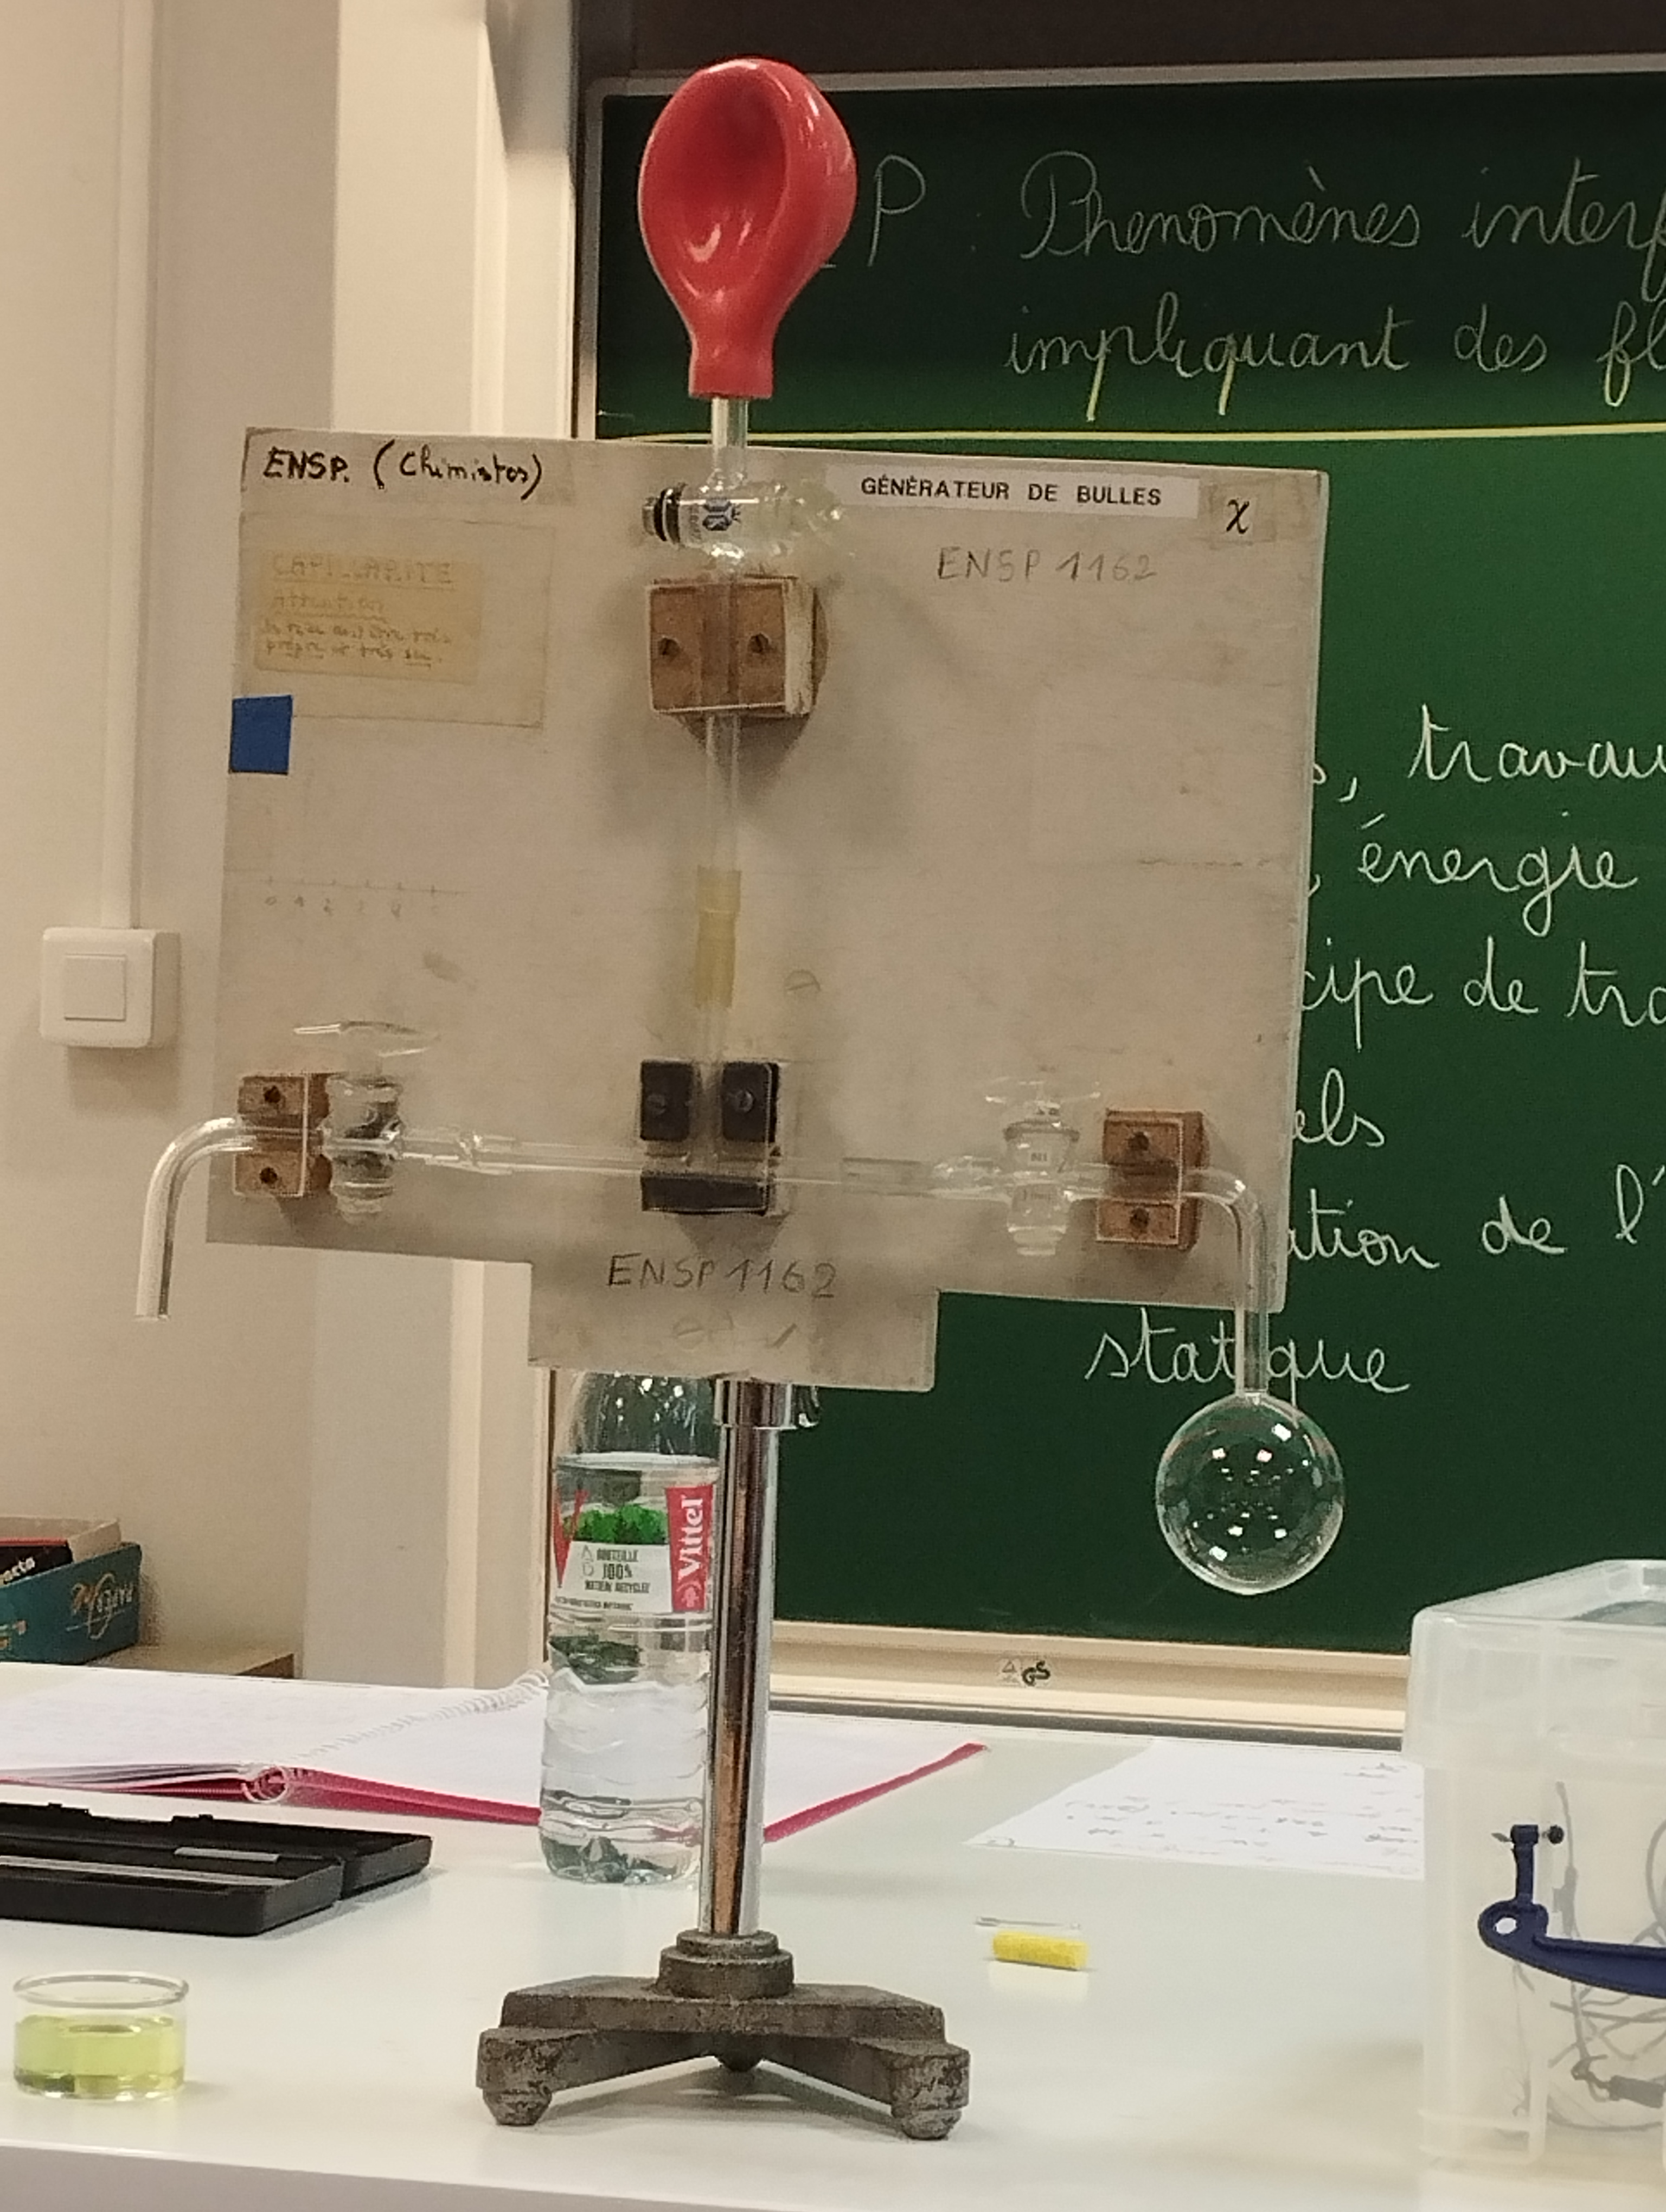
\includegraphics[scale=0.1]{LP_TensionSurface/Manip_Laplace.jpg}
     
 \end{center}
 La différence de pression avec l'extérieur est donc plus grande dans les petites bulles : on peut le démontrer mathématiquement via la \textbf{Loi de Laplace.}
 Pour cela, on applique le principe des travaux virtuels. On imagine qu'on accroît le rayon de la bulle de $dR$ sous une différence de pression $\Delta P = P_1-P_2$ constante. La valeur de $\Delta P$ correspondant à l'équilibre mécanique sera telle que la variation d'énergie totale $\delta W_{tot}$ correspondante est nulle. Celle-ci est la somme du :
 \begin{enumerate}
     \item travail des forces de pression $\delta W_p = -(P_1-P_2)d(\frac{4}{3}\pi R^3)$
     \item la variation d'énergie de surface de la sphère : $\delta W_s = 2d(4\pi R^2\gamma)$, le facteur 2 correspond au fait qu'il y a deux interfaces pour une bulle.
 \end{enumerate}
 A l'équilibre : $\delta W_p+\delta W_s =0$.  Finalement : 
 \textcolor{red}{Loi de Laplace : }
 \begin{equation}
     (P_1-P_2)=\frac{4\gamma}{R}
 \end{equation}
 \begin{itemize}
     \item Plus $R$ est petit, plus la pression à l'intérieur est grande. 
     \item Lorsque $R \rightarrow \infty$ (surface plane), on a continuité de la pression.
     \item Cette loi nous permet de mesurer $\gamma$ expérimentalement.
     \item Remarque : pour une goutte, il y a 1 interface liquide-air donc $(P_1-P_2)=\frac{2\gamma}{R})$
 \end{itemize}
 
 \subsection{Mesure de $\gamma_{savon-air}$}
 \textcolor{blue}{Expérience :}  Pour une bulle de savon, deux interfaces donc $\Delta P =\frac{4\gamma}{R}$. On génère une bulle, on mesure son rayon à l'aide d'un pied à coulisse et la pression à l'intérieur grâce à un manomètre différentiel. Il permet de mesurer la différence de pression entre l'intérieur de la bulle et l'extérieur à travers une mesure de tension (piézo). J'ai pris plusieurs points en préparation, je vais en prendre un devant vous. Une regression linéaire $\delta P = \frac{A}{R}$ permet d'obtenir $\gamma$. \textcolor{red}{Tracer plutôt $R=f(\Delta P)$ car incertitude max sur R.}\\

La pente de $\Delta P = 4 \gamma\times 1/R$ donne $\gamma=28.8 \pm 2.2$~mN/m$^2$ qui est plus faible que celle de l'eau dû à la présence d'un tensioactif (savon = tensioactif). Par ailleurs, on retrouve le bon ordre de grandeur pour une eau savonneuse (internet donne $25$~mN/m$^2$). \\

\subsection{Cas général (cette partie peut sauter)}
Faire la démo. 
\begin{center}
    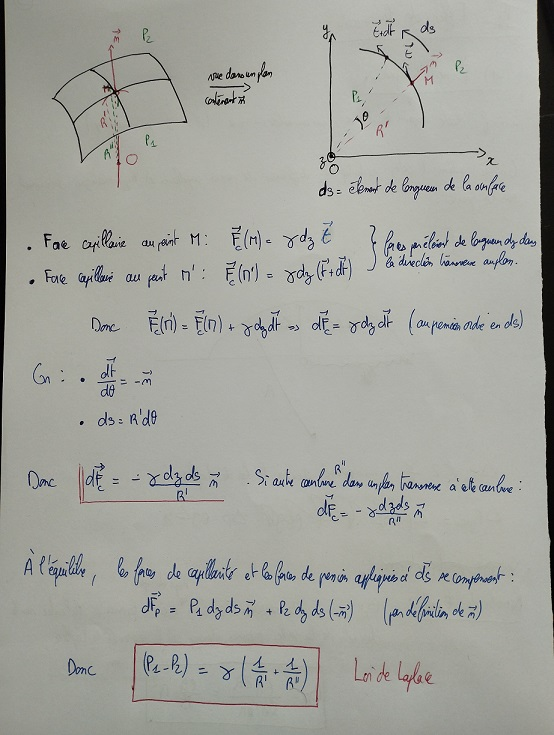
\includegraphics[scale=0.5]{LP_TensionSurface/Demo_Laplace.jpg}
\end{center}
Insister sur le caractère algébrique de R' et R". \textcolor{green}{Slide : Film de savon entre deux anneaux.}
Faire un schéma bulle normale, bulle caténoïde Pour la caténoïde, $\frac{1}{R}=-\frac{1}{R'}$ ce qui permet de satisfaire la loi de Laplace en tout point de l'interface dans le cas ou les pressions sont égales de part et d'autre.\\

\textcolor{red}{Transition : ce qu'on a vu dans cette partie c'est que les effets de capillarité sont directement reliés à la courbure des interfaces pour des petits objets. Mais pour des gros objets, il y a des effets de gravité qui s'ajoutent ce qu'on a vu dans l'expérience avec les bulles de savon.}

  \section{Influence de la gravité}
  
  \textcolor{green}{slide : gouttes de mercure sur une plaque de verre. Plus la taille de la bulle est grande, plus la forme sphérique est déformée.}
  Il y a un effet de gravité qui n'est plus négligeable à partir d'une certaine taille : laquelle ? C'est ce qu'on va voir dans cette partie.
  
  \subsection{Nombre de Bond}
  Considérons une goutte sphérique posée sur une surface plane solide. Cette goutte est plongée dans un fluide de masse volumique $\rho$ et possède une masse volumique $\rho+\Delta\rho$.\\
  
  La différence de pression hydrostatique au point M(z=h) de la goutte est donnée par la loi de l'hydrostatique :
  \begin{align}
      P_1+(\rho+\Delta\rho)gh &= P_2+\rho gh \\
      P_1-P_2 &= \Delta\rho gh = \Delta P_{grav}
  \end{align}
  La différence de pression capillaire à l'interface est donnée par la loi de Laplace :
  \begin{equation}
      P_1-P_2 = 2\frac{\gamma_{LG}}{R} = \Delta P_{cap}
  \end{equation}
  On définit le nombre de Bond $B_O$ comme le rapport entre ces deux différences de pression :
  \begin{equation}
     B_O = \frac{\Delta P_{grav}}{\Delta P_{cap}}\sim \frac{\Delta\rho gr_g^2}{\gamma} = \left(\frac{r_g}{l_c}\right)^2
  \end{equation}
  avec $r_g$ le rayon de la ligne de contact. On a définit ici une longueur appelée longueur capillaire $l_c=\sqrt{\frac{\gamma_{LG}}{\Delta\rho g}}$.
  Cela nous amène à distinguer deux cas :
  \begin{itemize}
      \item Si $l_c>>R$, alors les effets gravitaires sont dominants,
      \item Si $B_O<<1$, l
  \end{itemize}
  Compétition entre gravité et tension de surface : $B_0=\frac{\rho R^2g}{\gamma}$. La longueur capillaire $l_c$ est telle que: $B_0=\frac{\rho l_c^2g}{\gamma}=1$ (frontière entre les deux régimes), soit $l_c = \sqrt{\frac{\gamma}{\rho g}}$.
  Pour l'eau, $l_c=3$mm.\\
  Deux régimes : 
  \begin{itemize}
      \item $R>>l_c$, la gravité domine : goutte plate.
      \item $R<<l_c$, la tension de surface domine, la bulle est sphérique.
  \end{itemize}
  Photo ménisque : résulte de cette compétition entre tension de surface responsable de sa formation et gravité qui s'y oppose. Menisque concave pour un fluide mouillant (ex: eau dans tube en verre) et convexe pour un fluide peu mouillant (ex: mercure dans tube en verre)
  \begin{center}
      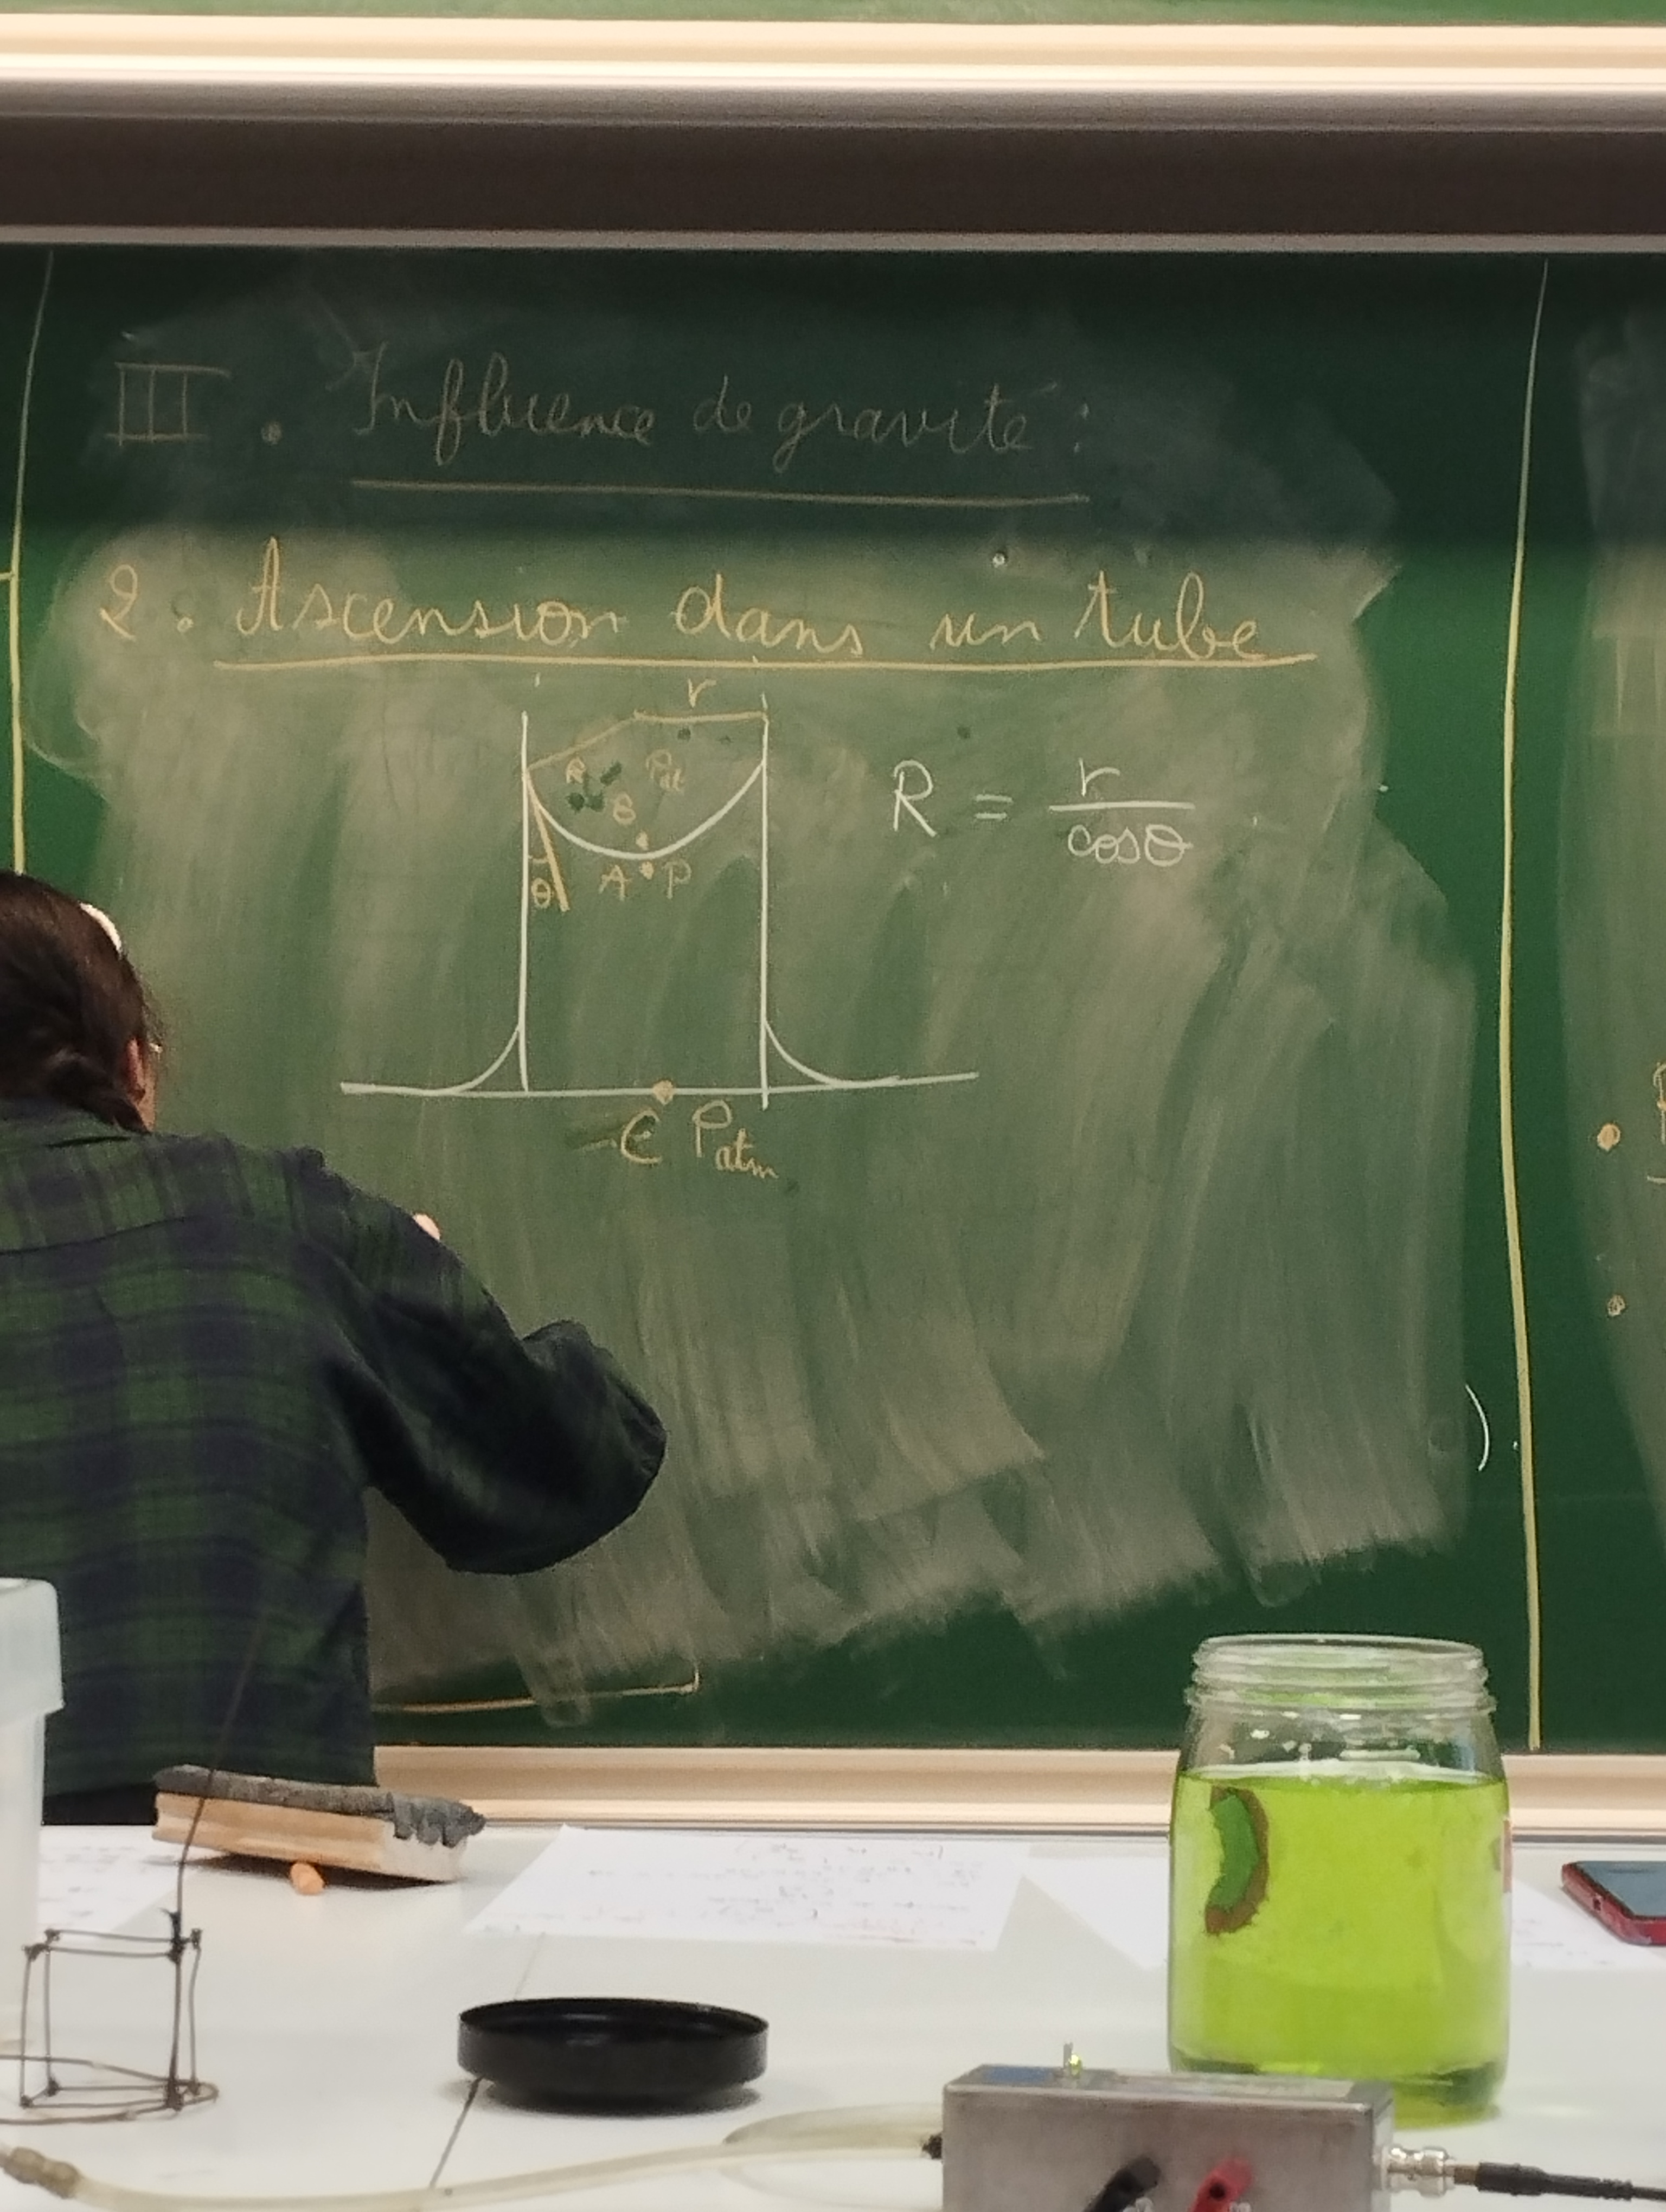
\includegraphics[scale=0.1]{LP_TensionSurface/Menisque.jpg}
  \end{center}

  \subsection{Ascension capillaire dans un tube}
  Vidéo de l'ascension d'un liquide dans différents tubes capillaires (voir site Laurent Le Guillou dans la partie TP). Plus le tube est fin, plus le liquide monte haute.
  Schéma liquide dans un tube de rayon $r$, rayon de courbure du ménisque $R$, angle de contact $\theta$. On applique la loi de Laplace : $\Delta P = \frac{2\gamma}{R}=\frac{2\gamma\cos(\theta)}{r}$. En appliquant l'équation de l'hydrostatique, on obtient \textcolor{red}{la Loi de Jurin} :
  \begin{equation}
      h = \frac{2\gamma\cos(\theta)}{\rho g r}
  \end{equation}
  En effet, plus $r$ est petit, plus $h$ est grand. Cette loi permet de mesurer $\gamma$.

\section{Effet de mouillage}
  \textcolor{green}{Mouillage :} étude de l'étalement d'un liquide sur un substrat (solide ou liquide). Utile dans l'industrie (peinture, encre, traitement des pneus, crème, maquillage, etc.).\\
  $\theta =$ angle de contact, permet de savoir si un liquide mouille plus ou moins bien un substrat. Résulte d'une compétition entre les tensions de surface intervenant dans les trois interfaces (L/G, L/S, S/G). \\
  \textbf{26min}\\
  Le système est \{\textbf{dl}$\in$ ligne triple\}. 
  $\textbf{dF}=0$ à l'équilibre. La projection sur l'axe du solide donne la \textcolor{red}{Loi de Young-Dupré} :
  \begin{equation}
      \gamma_{LG}\cos(\theta) = \gamma_{SG}-\gamma_{SL}
  \end{equation}
  
  \section*{Conclusion (40min)}
  Expérience de conclusion : Pince à nourrice dans eau flotte, puis coule avec tensio-actif (savon).



\end{reportBlock}


%%%%%%%%%%%%%%%%%%%%%%%%%%%%%%%%%%%%%%%%%%%%%%%%%%%%
%%%% Questions
\begin{reportBlock}{Questions posées par l’enseignant (avec réponses)}
  \textbf{C : C'est quoi un tensioactif ?} \textcolor{purple}{\'{E}lément qui diminue la tension de surface. Il est composé d'une tête hydrophile et d'une queue hydrophobe. La tête va se mettre à l'interface du côté de l'eau tandis que la queue sera du côté de l'air, faisant le lien entre l'eau et l'air. Cette configuration permet de diminuer l'énergie de l'interface, et donc diminue la tension de surface. } \newline

  \textbf{C : La dynamique de l'ascension dans la loi de Jurin semble diférrente en fonction du diamètre du tube ? Pouvez-vous discuter des éléments à prendre en compte pour essayer de comprendre pourquoi ça monte plus vite ou plus lentement ?} \textcolor{purple}{Plus le rayon est grand, plus la vitesse est grande. Peut se comprendre en ordre de grandeur via $\nabla P = \eta \Delta v$ soir $\frac{P}{h} \sim \eta \frac{v}{r^2}$}
  %En comparant à Poiseuille cylindrique, il y a une dépression à l'interface air/liquide qui fait augmenter brutalement la vitesse. Lorsque le liquide monte, le gradient de pression diminue ($\frac{\delta P}{\delta z}=\frac{2\gamma}{rh}$, r rayon du tube et h hauteur de l'ascension) et en prenant en compte la gravité et les forces de viscosité ($\frac{\delta^2v_r}{\delta z^2}$), ça va ralentir l'ascension.

  \textbf{C : Où placeriez-vous cette leçon dans le cours global de mécanique des fluides ?} \textcolor{purple}{Après l'équation de Navier-Stokes. C'est presque une domaine un peu à part.}

  \textbf{C : Peut-on imaginer qu'on n'ait pas de saut de pression à travers une surface courbe ?} \textcolor{purple}{En utilisant l'équation de Laplace pour une surface quelconque, $\Delta P =\gamma(1/R+1/R')$, R et R' sont les deux rayons de courbures de la surface en un point donné et sont algébriques (compté positivement si le centre de la coubure est à l'intérieur de la surface, négativement sinon. Par exemple, pour un point selle, on a $R' = -R$ impliquant une continuité de la pression.}

  \textbf{C : Dans l'équation de Young-Dupré, vous avez dessiné 3 forces mais il ne me semblait pas qu'on était en équilibre (au moins à la normale à la surface)} \textcolor{purple}{La force de réaction du support compense la composante normale de la force de tension de surface.}

  
  \textbf{C : D'autres façon pour déterminer $\gamma$ ?} \textcolor{purple}{Tensiomètre à plaque de Wilhelmy: on mesure la force exercée sur la plaque par le liquide grâce à une microbalance, et on peut en déduire $\gamma$.}

  
  \textbf{C : Dessin d'une goutte sur un plan incliné ? De quoi dépendrait l'angle d'inclinaison ?} \textcolor{purple}{Vitesse, viscosité, et coefficient de tension de surface.}

  
  \textbf{C : Pouvez-vous expliquer pourquoi on peut faire des chateaux de sables avec du sable mouillé ?} \textcolor{purple}{La présence d'eau va créer un pont capillaire entre deux grains qui va augmenter la force de cohésion entre les grains. Cette cohésion se fait sur une surface beaucoup plus grande pour le grain mouillée grâce au pont capillaire alors que pour un grain sec, cette cohésion se fait au niveau d'une rugosité (très petite surface) et donc insuffisance pour maintenir un château de sable.}



  \textbf{C : Pourquoi les serviettes sont rêches quand elle sèche ? Quel est le principe d"un adoucissant ?} \textcolor{purple}{Lorsqu'une serviette est mouillée, l'eau va chercher à minimiser son interface avec l'air en collant et écrasant les fibres de la serviette (c'est aussi pour ça que nos cheveux sont collés en sortant de la douche). En séchant, la serviette durcit, lui donnant une texture rêche. L'adoucissant agit chimiquement sur les fibres pour rendre le linge plus doux au toucher.}


  \textbf{C : $\gamma(T)$ ? Que se passe-t-il s'il y a des endroits du fluide qui sont plus chauds que d'autres ?} \textcolor{purple}{Création d'un gradient de tension de surface qui va causer un déplacement du liquide des zones de faibles $\gamma$ vers les zones de $\gamma$ élevée (cf. effet Marangoni).}

  
  \textbf{C : On parle parfois de liquide mouillant et de liquide non-mouillant. Valeurs de $\theta$ ?} \textcolor{purple}{Mouillage total : $\theta=0$, non-mouillage total : $\theta=\pi$.}

  
  \textbf{C : Commenter les incertitudes sur l'expérience ?} \textcolor{purple}{Incertitudes dominantes sur la mesure du rayon avec le pied à coulisse que j'ai pris de $0.5$mm, ce qui est une grande incertitude.}


  \textbf{C : Principe du manomètre ?} \textcolor{purple}{Un piézoélectrique subit une contrainte mécanique sous l'effet de la différence de pression, générant une tension que l'on mesure. Le constructeur nous donne la relation de conversion entre tension et pression.}

  \end{reportBlock}
  
%%%%%%%%%%%%%%%%%%%%%%%%%%%%%%%%%%%%%%%%%%%%%%%%%%%%
%%%% Commentaires
\begin{reportBlock}{Commentaires lors de la correction de la leçon}
Bonne leçon, beaucoup apprécié toutes les expériences montrées. Vous maîtrisez pas mal de choses. Attention à ce que le dispositif ne gène pas la vue sur le tableau.\\


\end{reportBlock}



%%%%%%%%%%%%%%%%%%%%%%%%%%%%%%%%%%%%%%%%%%%%%%%%%%%%
%%%% Correction
\begin{reportBlock}{Partie réservée au correcteur}
  \textbf{Avis général sur la leçon (plan, contenu, etc.) :}
  
  
  \textbf{Notions fondamentales à aborder, secondaires, délicates :}
  
  
  \textbf{Expériences possibles (en particulier pour l'agrégation docteur) :}
  
  
  \textbf{Bibliographie conseillée :}
\end{reportBlock}


\begin{reportBlock}{Partie réservée au correcteur}
  \textbf{Avis général sur la leçon (plan, contenu, etc.) :}
  
  
  \textbf{Notions fondamentales à aborder, secondaires, délicates :}
  
  
  \textbf{Expériences possibles (en particulier pour l'agrégation docteur) :}
  
  
  \textbf{Bibliographie conseillée :}
\end{reportBlock}
\newpage
%%%%%%%%%%%%%%%%%%%%%%%%%%%%%%%%%%%%%%%%%%%%%%%%%%%%
%%%% En-tête leçon
\begin{headerBlock}
    \chapter{Premier principe de la thermodynamique}
    \label{LP_PremierPrincipe}
\end{headerBlock}




%%%%%%%%%%%%%%%%%%%%%%%%%%%%%%%%%%%%%%%%%%%%%%%%%%%%
%%%% Références
\begin{center}
\begin{tabularx}{\textwidth}{| X | X | c | c |}
  \hline
  \rowcolor{gray!20}\multicolumn{4}{c}{Bibliographie de la leçon : } \\
  \hline 
  Titre & Auteurs & Editeur (année) & ISBN \\
  \hline
 Physique Tout en 1 MPSI PTSI & Bernard Salamito et al.  & Dunod &    \\
  \hline 
 Thermodynamique 1ère année MPSI-PCSI-PTSI & Jean-Marie Brébec  & H Prépa (Hachette Supérieur)  &    \\
  \hline 
 &   &   &    \\
  \hline 
 &   &   &    \\
  \hline
\end{tabularx}
\end{center}

%%%%%%%%%%%%%%%%%%%%%%%%%%%%%%%%%%%%%%%%%%%%%%%%%%%%

%%%%%%%%%%%%%%%%%%%%%%%%%%%%%%%%%%%%%%%%%%%%%%%%%%%%
%%%% Plan
\begin{reportBlock}{Plan détaillé}
  \textbf{Niveau choisi pour la leçon :} 1ère année de CPGE
  \newline
  \textbf{Prérequis :} Système thermodynamique fermé ; Transformation thermodynamique quasi-statique ; Fonctions d'état ; Equilibre thermodynamique ; Energies cinétique et potentielles, Travail d'une force 
  \newline
  
  \textbf{Déroulé détaillé de la leçon: }   \newline
  
  \section*{Introduction (3min)}
 La thermodynamique classique est une branche de la physique qui s'intéresse aux propriétés macroscopiques d'un système, et qui étudie les transformations de la matière et les échanges d'énergie sous différentes formes entre ce système et son environnement sans chercher à comprendre ce qui se passe au niveau microscopique. C'est une théorie axiomatique basée sur principalement sur deux principes.\\
  Animation : https://phet.colorado.edu/sims/html/energy-forms-and-changes/latest/energy-forms-and-changes\_en.html. Pour un système isolé, l'énergie ne se créé pas et ne disparaît pas, mais elle se transforme d'une forme à une autre : Ex animation : conversion énergie mécanique-électrique, électrique-thermique. \\
  Si le système est isolé, il y a conservation de l'énergie.  \\
  Leçon placée en 1re année CPGE. Review des prérequis.
  
  \section{Premier principe de la thermodynamique}
  Système ($\Sigma$) fermé.
  
  \subsection{Enoncé} Il existe une fonction d'état extensive \textbf{U} appelée énergie interne, telle que : 
  \begin{equation}
      \Delta E = \Delta E_c + \Delta E_p + \Delta U = W + Q
  \end{equation}
  \textcolor{red}{Interprétation :}
  \begin{itemize}
  \item U : $\sum_{i} E_{c,micro} + E_{p,micro}$
  \item $E_c$ : énergie cinétique macroscopique
  \item $E_p$ : énergie potentielle macroscopique (ex : $E_p=mgz$)
  \item $W$ : travail des forces macroscopiques extérieures non conservatives
  \item $Q$ : transfert thermique (chaleur) dû à l'agitation thermique aléatoire des particules
  \end{itemize}
  $Q$ et $W$ deux modes de transferts d'énergie. Ils sont algébriques (comptés positivement si reçus par le système. \\
  
  \textcolor{red}{Conséquences : } Si système isolé : $\Delta E = 0$ (conservation de l'énergie). \\
  
  \textcolor{red}{Version infinitésimale : } $dE_c + dE_p + dU = \delta W + \delta Q$.
  
  \subsection{Travaux des forces de pression (11min30)}
  Schéma fluide contenu dans une paroi. Pression extérieure $P_e$ uniforme et constante. Système = {fluide + paroi}. Variation du volume total de $dV$ entre entre $t$ et $t+dt$. En $M$ déplacement de $\mathbf{dM}$. \\
  Force apppliquée au système en un point $M$ : $\mathbf{dF}=-P_e\mathbf{dS}$. Travail asssocié $\delta^2 W = \mathbf{dS}\cdot\mathbf{dM} = -P_e \mathbf{dS}\cdot\mathbf{dM} = - P_e d^2 V$. Travail totale $\delta W$ s'obtient en sommant les travaux : $\delta^2 W$ $\delta W = -P_e dV$\\
  \underline{Si transformation quasi-statique et équilibre mécanique avec l'extérieur $P=P_e$} $\delta W = - p \ud V$ et $W = - \int_A^B p \ud V$ entre deux états $A$ et $B$.
  
 \subsection{Exemples de bilan d'énergie}
 \subsubsection{Trasformation isochore}
 $dV=0$ d'où $W=0$ donc $\Delta U = Q$.
 
 \subsubsection{Transformation monobare et enthalpie}
 $P_e=cste$ donc $W=-P_e(V_f-V_i)$ donc $\Delta U = Q + W$ donc $Q = \Delta U - W = [U_f +P_f V_f]-[U_i+P_iV_i] = H_f - H_i$.\\
 On définit l'enthalpie $H=U+PV$.\\
 
 \textcolor{red}{Premier Principe (transormation monobare):} $\Delta H = Q + W_{autre}$.
 
  \section{Applications du premier principe (20min)}
  \subsection{Définitions préliminaires}
  \textcolor{red}{Capacité thermique à volume constant : } $C_V = (\frac{\partial{U}}{\partial{T}})_V \rightarrow c_V = \frac{C_V}{m}$. \\
  \textcolor{red}{Capacité thermique à pression constante : } $C_P = (\frac{\partial{H}}{\partial{T}})_V \rightarrow c_P = \frac{C_P}{m}$. \\
  
  \subsection{Calorimétrie (24min)}
  \textcolor{red}{Expérience} Vase Dewar avec agitateur permettant d'homogénéiser le contenu. On peut remonter à la capacité calorifique.  La pression extérieure est fixée : transformation monobare. On suppose la transformation adiabatique : $\Delta H = Q = 0$.\\
  Pour le système \{eau+calorimètre+fer\} : $\Delta H = \Delta H_{eau} + \Delta H_{calo} + \Delta H_{fer} = c_{eau}\times m_{eau}\times \Delta T_{eau} + c_{eau}\times \mu \times \Delta T_{cal} + c_{fer}\times m_{fer}\times \Delta T_{fer}$.\\
  $\mu =29(3)$ déterminé en préparation. Mesure des masses à la balance : $m_{eau}$ et $m_{fer}$ ; et mesure des températures au thermocouple : $T_{eau+cal}$ et $T_{fer}$ à l'état initial et  $T_f$ à l'état final.\\
  On en déduit : $c_{fer}=\frac{c_{eau}(m_{eau}+\mu)(T_{eau+cal}-T_f)}{m_{fer}(T_f-T_i)}=1016\pm 184$~J.kg$^{-1}$.K$^{-1}$ à comparer à $c_{fer}=449$~J.kg$^{-1}$.K$^{-1}$.\\
  
  \subsection{Détente de Joule - Gay Lussac (38min)}
  Deux enceintes séparées par un robinet. Une enceinte est remplie par un gaz, l'autre par un fluide. Ces enceintes sont calorifugées et avec des parois rigides. On ouvre le robinet. \\
  Système = {gaz+vide+enceintes}. On a $\Delta U=0$. Si $U(T)$ (première loi de Joule) : $\Delta U = C_{V}\Delta T = 0$ donc transformation isotherme. \\
  Cette expérience permet de vérifier si un gaz vérifie la première loi de Joule en mesurant la variation de température.
  
  \section*{Conclusion (40min)}
  Dans cette leçon, on a parlé du premier principe qui est un principe de conservation de conservation. Ce principe est complété par le second principe, qui lui, est plutôt un principe d'évolution et qui porte sur le caractère réversible ou irréversible d'une transformation. Pour finir, ces principes et la thermodynamique classique en général a été formalisée plus tard par la mécanique statistique qui permet d'expliquer les résultats de la thermodynamiques en faisant le lien entre l'échelle microscopique et macroscopique.



\end{reportBlock}


%%%%%%%%%%%%%%%%%%%%%%%%%%%%%%%%%%%%%%%%%%%%%%%%%%%%
%%%% Questions
\begin{reportBlock}{Questions posées par l’enseignant (avec réponses)}
  \textbf{C : Sur la vidéo, comment on fait conversion énergie mécanique et électrique ?}  \textcolor{purple}{Avec un alternateur : un aimant est entrainé par l'énergie mécanique qui créé un courant variable dans une bobine par induction. Exemple : une dynamo de bicyclette. Si pas de champs magnétiques préexistant, induction électromagnétique.} \newline
  
  \textbf{C : Dans l'énoncé du premier principe, quelles sont les particularités de A et B ?}  \textcolor{purple}{Ils sont à l'équilibre thermodynamique pour qu'on puisse leur défiir une énergie .} \newline
  
  \textbf{C : W est le travail des forces non conservatives ? Si je prends un piston qui est bloqué par un poids, il y a le poids dans W ? Si j'ajoute une force, ça agit sur E$_p$ par sur U (par exemple la force de Lorentz qui agit sur chaque particule ?}  \textcolor{purple}{Il est bien présent dans la partie gauche de l'équation. Si on le met à doite ça agit sur $E_p$ et on met un signe \og - \fg. C'est un peu indifférent de le mettre à droite où à gauche mais il ne faut pas le compter deux fois et mettre le bon signe. } \newline
  
  \textbf{C : De façon non ambigüe, peut-on mesurer une quantité de chaleur ou savor ce que c'est ?}  \textcolor{purple}{La chaleur ça sera toute la variation d'énergie sauf le travail des forces macroscopiques. On peut mesurer la variation d'énergie interne dans certaines conditions.} \newline
  
  \textbf{C :Si transfo quasi-statique, on peut faire $-P_edV$. Peut-on juste dire que la transformation est réversible ?}  \textcolor{purple}{Oui ça fonctionne mais dans la vie il n'existe pas de transformation réversible.} \newline
  
  \textbf{C : Définition de réversible ?}  \textcolor{purple}{On peut changer le sens et changeant infiniment peu les contraintes extérieures. On peut prendre l'exemple d'un piston où il y a des frottements pour la différence entre réversible et quasi-statique.} \newline
  
  \textbf{C : Dans la détente Joule Gay Lussac, est-ce que c'est important que l'enceinte soit vide ou remplie d'un gaz à pression plus faible par exemple ?}  \textcolor{purple}{Il faut juste faire attention à la définition du système. } \newline
  
  \textbf{C :Si on veut une variation de chaleur $\delta Q$ pour un fluide, quels sont les coefficients importants ?}  \textcolor{purple}{Il y a 6 variables calorimétriques importantes. Suivant le système, il faut prendre la dépendance en volume etc... On peut montrer qu'il n'y en a que deux d'indépendantes.} \newline
  
  \textbf{C :Différentes façon d'exprimer $\delta Q$ : $\delta Q = c_vdT + ldV = c_pdT + hdP = \lambda dP + \mu dV$. On peut montrer la relation entre pente adiabatique et pente isotherme. Quelle est la pente la plus importante entre une adiabatique ou une isotherme dans le diagramme (P,V) ? Calculer la pente pour une adiabatique et une isotherme ? }  \textcolor{purple}{Isotherme : $dT=0$ donc $\delta Q= ldV = hdP$. Adiabatique : $dV = -\frac{c_v}{l}dT$ et $dP = -\frac{c_p}{h}dT= \frac{c_pl}{hc_v}dV$.} \newline
  
  \textbf{C :Comment exprimer de manière générale $dP$ en fonction de $dT$ et $dV$ à partir d'une équation d'état ?}  \textcolor{purple}{$dT = (\frac{\partial{T}}{\partial{P}})_VdP + (\frac{\partial{d}T}{\partial{d}V})_VdV$. On en déduit } \newline
  
  \textbf{C :Dans le diagramme (P,V), on considère des transformations infinitésimales entre A et D (entre A et B : isochore, B et C : isobare, C et D : isotherme et entre D et A : isobare). Calculer la variation infinitésimale $\delta Q$ sur le cycle en commençant d'abord par les chemins A-B-C et A-D-C.}  \textcolor{purple}{Sur A-B-C : $\delta Q = \lambda dP + \mu dV$. Sur A-D-C, $\delta Q = c_pdT + hdP$. Donc sur le cycle : $\delta Q = -\delta W = \lambda dP + \mu dV - c_pdT - hdP$. } \newline
  
  
\end{reportBlock}


%%%%%%%%%%%%%%%%%%%%%%%%%%%%%%%%%%%%%%%%%%%%%%%%%%%%
%%%% Commentaires
\begin{reportBlock}{Commentaires lors de la correction de la leçon}
Très bonne leçon. Basile : je n'aurai pas du tout évoquer le terme chaleur.\\
Pour l'expérience, on aurait pu faire l'inverse en faisant chauffer la barreau de fer et mettre de l'eau à température ambiante. Il y aurait peut-être moins de pertes.\\
Tu as parlé moins vite et c'était mieux par rapport à la dernière fois.\\
Pas de forces à longue portée pour que U soit extensive.


\end{reportBlock}



%%%%%%%%%%%%%%%%%%%%%%%%%%%%%%%%%%%%%%%%%%%%%%%%%%%%
%%%% Correction
\begin{reportBlock}{Partie réservée au correcteur}
  \textbf{Avis général sur la leçon (plan, contenu, etc.) :}
  
  
  \textbf{Notions fondamentales à aborder, secondaires, délicates :}
  
  
  \textbf{Expériences possibles (en particulier pour l'agrégation docteur) :}
  
  
  \textbf{Bibliographie conseillée :}
\end{reportBlock}


\begin{reportBlock}{Partie réservée au correcteur}
  \textbf{Avis général sur la leçon (plan, contenu, etc.) :}
  
  
  \textbf{Notions fondamentales à aborder, secondaires, délicates :}
  
  
  \textbf{Expériences possibles (en particulier pour l'agrégation docteur) :}
  
  
  \textbf{Bibliographie conseillée :}
\end{reportBlock}
\newpage
%%%%%%%%%%%%%%%%%%%%%%%%%%%%%%%%%%%%%%%%%%%%%%%%%%%%
%%%% En-tête leçon
\begin{headerBlock}
  \chapter{Transition de phase}
  \label{LP_TransitionPhase} 
\end{headerBlock}




%%%%%%%%%%%%%%%%%%%%%%%%%%%%%%%%%%%%%%%%%%%%%%%%%%%%
%%%% Références
\begin{center}
\begin{tabularx}{\textwidth}{| X | X | c | c |}
  \hline
  \rowcolor{gray!20}\multicolumn{4}{c}{Bibliographie de la leçon : } \\
  \hline 
  Titre & Auteurs & Editeur (année) & ISBN \\
  \hline
  Thermodynamique & BFR & Dunod & \\
  \hline 
  Thermodynamique & Diu &  &    \\
  \hline 
   &  & &    \\
  \hline 
\end{tabularx}
\end{center}

%%%%%%%%%%%%%%%%%%%%%%%%%%%%%%%%%%%%%%%%%%%%%%%%%%%%

%%%%%%%%%%%%%%%%%%%%%%%%%%%%%%%%%%%%%%%%%%%%%%%%%%%%
%%%% Plan
\begin{reportBlock}{Plan détaillé}

  \textbf{Niveau choisi pour la leçon :} Licence 3
  \newline
  \textbf{Prérequis} : \begin{itemize}
      \item 
  \end{itemize}

  \textbf{Déroulé détaillé de la leçon: }  
  
  \section*{Introduction}

  \section{Transition de phase du 1er ordre}
  \subsection{Enthalpie de changement d'état} 


  \section{Transition de phase du 2nd ordre}
\subsection{Transition paramagnétisme-ferromagnétisme}


\end{reportBlock}
\newpage
%%%%%%%%%%%%%%%%%%%%%%%%%%%%%%%%%%%%%%%%%%%%%%%%%%%%
%%%% En-tête leçon
\begin{headerBlock}
  \chapter{Phénomènes de transport}
    \label{LP_Transport}
\end{headerBlock}

%%%%%%%%%%%%%%%%%%%%%%%%%%%%%%%%%%%%%%%%%%%%%%%%%%%%
%%%% Références
\begin{center}
\begin{tabularx}{\textwidth}{| X | X | c | c |}
  \hline
  \rowcolor{gray!20}\multicolumn{4}{c}{Bibliographie de la leçon : } \\
  \hline 
  Titre & Auteurs & Editeur (année) & ISBN \\
  \hline
  Thermodynamique & BFR & Dunod (1989) & \\
  \hline
  Thermodynamique & Diu & & \\
  \hline 
  Tout-en-un PC/PC* & M.-N. Sanz & Dunod (2022) & \\
  \hline 
  Ondes mécaniques et diffusion & Christian Garing & Ellipses (1998) & \\
  \hline
\end{tabularx}
\end{center}

\begin{reportBlock}{Commentaires des années précédentes :}
    \begin{itemize}
        \item \textbf{2017 :} La leçon ne peut se limiter à la présentation d’un unique phénomène de transport
        \item \textbf{2016 :} Les analogies et différences entre les phénomènes de transport doivent être soulignées tout en évitant de dresser un simple catalogue,
        \item \textbf{2015 :} Les liens et les limites des analogies entre divers domaines doivent être connus
    \end{itemize}
\end{reportBlock}


%%%%%%%%%%%%%%%%%%%%%%%%%%%%%%%%%%%%%%%%%%%%%%%%%%%%
\begin{reportBlock}{Plan détaillé}
  \textbf{Niveau choisi pour la leçon :} Prépa deuxième année
  \newline
  \textbf{Prérequis : }
  \newline

\section*{Introduction}
Les principes de la thermodynamique utilisent la notion de fonction d'état qui permettent de décrire les transformations entre deux états d'équilibre sans se soucier du chemin qu'emprunte le système au cours de cette transformation. On va ici lever l'hypothèse de l'équilibre thermodynamique et on va s'intéresser à décrire le transport de quantité physiques comme la quantité de matière ou la température par exemple avant que le système atteigne macroscopiquement son équilibre ou qu'on lui impose des conditions aux limites.\\

\textcolor{blue}{Manip qualitative :} Mettre une goutte de sirop coloré dans de l'eau.\\

\textcolor{blue}{Expérience qualitative :} Barreau  chauffé + caméra thermique.

\section{Equilibre thermodynamique local (max 10min)}

\subsection{Système hors équilibre}
Cf Sanz Dunod p120. En première année, on définit 3 échelles de longueur :
\begin{itemize}
    \item échelle microscopique : taille caractéristique $\delta$ = distance moyenne entre deux particules pour liquide/solide, libre parcours moyen pour un gaz
    \item échelle macroscopique : taille L typique de système étudié
    \item échelle mésoscopique : échelle intermédiaire de taille $d$ telle que $\delta<<d<<L$.
\end{itemize}
Interpréter les expériences avec ces 3 trois échelles. La température de l'eau fait chauffer les barreaux, il y a un gradient de température qui se fait de la zone la plus chaude à la zone la plus froide. De même, il y a une propagation des molécules de sirop des zones de forte à faible concentration de ces molécules. \\

La température n'est pas la même sur toute la longueur des barreaux comme la densité de molécules dans le verre d'eau. Cependant on peut quand même définir sur des zones de faibles épaisseurs (faibles devant l'échelle de variation caractéristique de la température du barreau, ici par exemple une ligne horizontale de pixels) les variables d'états de la thermodynamique (température, pression, densité de particule, ...).

\subsection{Equilibre thermodynamique local}
Décrire des volumes mésoscopiques dans un volume macroscopique. D'après Diu p464 : \textcolor{green}{slide :} "lors d'un processus hors équilibre, il y a équilibre thermodynamique local si tout sous-système macroscopique infinitésimal (ou volume mésoscopique) peut-être regardé comme ayant atteint l'équilibre thermodynamique ". Une variable d'état $Y$ peut donc être définie localement $Y(M,t)$ en un point M du système macro, à l'instant t. Hypothèse valable si le déséquilibre \og n'est pas trop \fg c'est-à-dire :
\begin{itemize}
    \item l'équilibre thermo local règne partout dans le système,
    \item les écarts à l'équilibre sont suffisament faible pour qu'on puisse les traiter au premier ordre : \textcolor{red}{approximation linéaire}
\end{itemize}

Comment peux-t'on décrire physiquement la variation des variables d'états ? 

\subsection{Flux et courants}
\textcolor{green}{Définition :} Le flux, noté $\Phi(t)$, il s'agit d'un débit (de particules, d'énergie, de charges, ...) à travers une surface $\mathcal{S}$ à l'instant t. Il est relié au vecteur densité de courant $\mathbf{j}$ dont le flux (au sens mathématique) à travers cette surface est :
\begin{equation}
    \Phi = \iint_{M\in\mathcal{S}}\mathbf{j}\cdot d\mathbf{S_M}
\end{equation}
Note : c'est une grandeur algébrique, positive si le courant rentre dans le système, négative s'il sort.\\

\textbf{Transition :} Maintenant qu'on a décrit le cadre physique pour décrire un phénomène de transport, on va l'appliquer dans un cas précis. J'ai choisi dans cette leçon de traiter le phénomène de diffusion de particules (le sirop dans l'eau).

\section{Diffusion de particules}

\subsection{Loi de conservation}
Sans production ou disparition de particules, faire un bilan :
\begin{itemize}
    \item soit global p94 Dunod 2016 et utiliser le théorème de Green-Ostrogradsky pour avoir la loi locale
    \item soit local à une dimension proprement (de préférence)
\end{itemize}
Expliquer qu'on décrit le transport de grandeurs \textbf{extensives et conservées}.

\subsection{Loi de Fick (1855)}
On a (comme pour le courant de charge en électromag) :
\begin{equation}
    \mathbf{j}(M,t) = n(M,t)\mathbf{v}(M,t)
\end{equation}
Problème, on retrouve avec une équation pour 4 inconnues (n, $j_x$, $j_y$ et $j_z$). Il manque une équation vectorielle. Enoncer la loi phénoménologique de Fick qui se constate expérimentalement :
\begin{equation}
    \mathbf{j}(M,t) = -D\grad{n(M,t)}
\end{equation}
avec $D$ le coefficient de diffusion (en m$^2$.s$^{-1}$). On note le signe \og - \fg~ devant le gradient qui s'explique naturellement par les expériences du début.\\

Donner le tableau odg (\textcolor{blue}{slide}) cf Dunod p96.\\


\subsection{Equation de diffusion}
(Démo possible p533 Diu)
On trouve : 
\begin{equation}
    \partialD{n}{t} = D\partialD{^2n}{x^2}
\end{equation}
$t\longleftrightarrow -t$ change l'équation : irréversibilité du phénomène de diffusion (déjà présent dans la loi de Fick).\\
Analogie : effet de peau dans un conducteur (équation de Maxwell-Ampère dans un plasma), diffusion de la quantité de mouvement et de vorticité au sein des fluides visqueux (faible nombre de Reynold).

\subsection{Mesures du coefficient de diffusion eau-glycérol}
Cf calcul compo 2002 agrégation standard partie D p14.

\subsection{Interprétation microscopique de la diffusion de particule (bonus)}
Cf Christian Garing p228-229 + code Python pour la diffusion p101 Dunod.

\section{Correspondance avec d'autres phénomènes de diffusion}

Faire un tableau. Critiquer loi d'Ohm qui provient d'une interaction des charges à longue portée, pas d'un mouvement brownien.

\section*{Conclusion}
Ouvrir sur le transport de plusieurs grandeurs couplées (effets thermoélectriques mais c'est chaud voir p515-521 Diu)
\end{reportBlock}
\newpage
%%%%%%%%%%%%%%%%%%%%%%%%%%%%%%%%%%%%%%%%%%%%%%%%%%%%
%%%% En-tête leçon
\begin{headerBlock}
  \chapter{Conversion de puissance électromécanique}
    \label{LP_ConversionPuissance}
\end{headerBlock}

%%%%%%%%%%%%%%%%%%%%%%%%%%%%%%%%%%%%%%%%%%%%%%%%%%%%
%%%% Références
\begin{center}
\begin{tabularx}{\textwidth}{| X | X | c | c |}
  \hline
  \rowcolor{gray!20}\multicolumn{4}{c}{Bibliographie de la leçon : } \\
  \hline 
  Titre & Auteurs & Editeur (année) & ISBN \\
  \hline
  TP Moteur &  & Site agreg Montrouge &   \\
  \hline 
  Cours Jérémy Neveu & J. Neveu & Site agreg Montrouge & \\
  \hline
  Tout-en-un PSI/PSI* (Chap 27 et 28) & S. Cardini & Dunod (2022) & \\
  \hline
\end{tabularx}
\end{center}

%%%%%%%%%%%%%%%%%%%%%%%%%%%%%%%%%%%%%%%%%%%%%%%%%%%%
\begin{reportBlock}{Plan détaillé}
  \textbf{Niveau choisi pour la leçon :} 
  \newline
  \textbf{Prérequis : }
  \newline

\section*{Introduction}
Parler de l'intérêt dans la vie de tous les jours :
\begin{itemize}
    \item Conversion mécanique - électrique : ex : éolienne, production d'électricité, courants de Foucault
    \item Conversion électrique - mécanique : moteur, haut-parleur, freinage par courants de Foucault
\end{itemize}

\section{Principe de la conversion}
\subsection{Exemple du rail de Laplace}
Faire le schéma en faisant attention à la convention d'orientation : choisir U et I, le reste c'est avec le bonhomme de Maxwell la règle de la main droite.\\

Neutralité du conducteur : $\rho_{e^-}=\rho_{ions}$ implique que la force de Lorentz s'écrit comme la force de Laplace $d\mathbf{F_{L}}=\mathbf{j}d\tau\wedge\mathbf{B}=I\mathbf{dl}\wedge\mathbf{B}$.\\

\subsection{Bilan de puissance}
Puissance mécanique : $dP_L = d\mathbf{F_{L}}\cdot\mathbf{v}=-I(\mathbf{v}\wedge\mathbf{B})\cdot\mathbf{dl}$. Comme le champ électromoteur s'écrit par définition : $\mathbf{E_m}=\mathbf{v}\wedge\mathbf{B}-\partialD{\mathbf{A}}{t}$, et la force électromotrice s'écrit $e=\mathbf{E_m}\cdot\mathbf{dl}$, on a \textcolor{red}{\underline{\textbf{en régime permanent }}} la relation fondamentale de conversion de puissance électromécanique :
\begin{equation}
    dP_L=-Ide\Rightarrow \boxed{P_{L} + P_{e} = 0}
\end{equation}
\importantbox{I est dans le sens de $\mathbf{dl}$}.

\subsection{Interprétation}
Deux cas de figure :
\begin{itemize}
    \item Pour un circuit électrique mobile dans un champ B permanent, si de la puissance électrique est fourni au circuit via des phénomènes d'induction ($P_e>0$) alors la même puissance est retirée du système mécanique ($P_L<0$). Par exemple, les moteurs.
    \item Si de la puissance est fourni au système mécanique via des forces de Laplace ($P_L>0$) alors la même puissance est retirée du système électrique via des phénomènes inductifs ($P_e<0$). Par exemple : les alternateurs dans les éoliennes/centrales électrique pour produire de l'électricité.
\end{itemize}

\textbf{Transition :} On va étudier dans une deuxième partie le principe du moteur à courant continu.

\section{Moteur à courant continu}
Cf cours de Jérémy.\\
Intérêt : commander la vitesse de rotation de l'arbre du moteur par la tension qu'on lui impose. Utilser pour les moteurs de faibles puissance (jusqu'à une centaine de kW).
\subsection{Structure}
\textcolor{blue}{Expérience qualitative :} Montrer le MCC de la collection. Décrire le stator, rotor, collecteur-balais. Shéma à une spire (cf Cours Jérémy Neveu).\\
Arriver sur les relations fondamentales du MCC :
\begin{align}
    E &= K\Phi_S\Omega \\
    <\Gamma(t)> &= K\Phi_SI_R
\end{align}
    
\subsection{Etude du MCC}
Avantage du moteur synchrone : réversible (si mode générateur : alternateur)
Attention : utiliser des multimètres métrix, poids de 100g à 5kg (x2 à chaque fois). Pied à coulisse pour $r$, chrono pour mesure $\Omega$ à la main, typiquement $v$ stable pour $\Delta x=10$~cm (cf tracker).\\
\textcolor{blue}{Manip 1 : }Déterminer $K_{em}$ la résistance du moteur et la comparer à la valeur donnée dans la notice. Je trouve $K_{em}=1.30(2)$~V.rad.s$^{-1}$.\\
\textcolor{blue}{Manip 2 :} Tracer $\eta$ en fonction de la puissance utile et comparer à charge nominale = 2kg et $\eta_{nom}=50\%$. Le courant lu est assez critique, ne pas hésiter à refaire plusieurs fois.\\

\textcolor{yellow}{Bonus :} Montrer la réversibilité du moteur avec une charge lourde pour voir apparaître ue tension lors de la descente.
\textbf{Transition : }Nous voyons bien que nous n'avons pas un rendement de 100\%, il y a des pertes.
\subsection{Bilan de puissance}
Faire schéma fonctionnnement du moteur (cf Tout-en-un PSI/PSI* p818).
\begin{itemize}
    \item Pertes cuivre : effet Joule dans les conducteurs constituant les bobinages de la machine,
    \item Pertes fer : puissance dissipée par le parcourt du cycle d'hystérésis des aimants en fer doux + puissance dissipée par effet Joule par les courants de Foucault 
    
\end{itemize}

\textbf{Transition :} Ces moteurs sont aujourd'hui mis en concurrence par les moteurs à courant alternatif dont nous allons détailler le fonctionnement pour les moteurs synchrones 

\section{Machines synchrones}
\subsection{Génération d'un champ magnétique tournant (bonus ?)}
\subsection{Champ rotorique et champ statorique}
\subsection{Point de fonctionnement et stabilité}

\section*{Ouverture}
Moteur asynchrone.
\end{reportBlock}
\newpage
%%%%%%%%%%%%%%%%%%%%%%%%%%%%%%%%%%%%%%%%%%%%%%%%%%%%
%%%% En-tête leçon
\begin{headerBlock}
 \chapter{Induction électromagnétique}
 \label{LP_Induction}
\end{headerBlock}

%%%%%%%%%%%%%%%%%%%%%%%%%%%%%%%%%%%%%%%%%%%%%%%%%%%%
%%%% Références
\begin{center}
\begin{tabularx}{\textwidth}{| X | X | c | c |}
  \hline
  \rowcolor{gray!20}\multicolumn{4}{c}{Bibliographie de la leçon : } \\
  \hline 
  Titre & Auteurs & Editeur (année) & ISBN \\
  \hline
   Electromagnatisme 3 : magnétostatique, induction, équations de Maxwell et compléments électroniques & M. Bertin, J. P. Faroux, J. Renault & Dunod Université (1986) & 2-04-016916-4 \\
  \hline 
   Physique Spé. MP*, MP et PT*, PT & Hubert Gié, Jean-Pierre Sarmat, Stéphane Olivier, Christophe More & Editions Tec \& Doc (2000) & 2-7430-0398-7 \\
  \hline 
   Physique Spé. PSI*, PSI & Stéphane Olivier, Christophe More, Hubert Gié & Editions Tec \& Doc (2000) & 2-7430-0399-5 \\
  \hline 
\end{tabularx}
\end{center}

%%%%%%%%%%%%%%%%%%%%%%%%%%%%%%%%%%%%%%%%%%%%%%%%%%%%

%%%%%%%%%%%%%%%%%%%%%%%%%%%%%%%%%%%%%%%%%%%%%%%%%%%%
%%%% Plan
\begin{reportBlock}{Plan détaillé}
  \textbf{Niveau choisi pour la leçon :} L3
  \newline
  \textbf{Prérequis : } Equations de Maxwell ; Forces de Lorentz, de Laplace ; ARQS magnétique ; Potentiels scalaire et vecteur ; Electrocinétique
  \newline
  
  \textbf{Déroulé détaillé de la leçon: }\newline
  \textbf{0. Introduction} 
  \begin{itemize}
      \item \textbf{Cadre général :} ARQS magnétique
      \item \textbf{Introduction historique :} Oersted (1820): courants éléctriques induisent $\mathbf B$. Faraday (1831): Variations de $\mathbf B$ qui induisent des courants électriques. 
  \end{itemize}
  \vspace{1cm}
  \textbf{I. Approche expérimentale} 3min20
  \begin{itemize}
      \item \textbf{Expérience qualitative 1:} Approche un aimant et éloigne un aimant droit d'une bobine fixe branchée à un oscilloscope : apparition d'une tension. Même observation avec déplacement de la bobine dans aimant fixe. Amplitude de l'intensité proportionnelle à la vitesse de variation de $\mathbf B$.
      \item \textbf{Définition générale de l'induction (slide)} apparition d'une f.e.m et, s'ils peuvent s'écouler, de courants, dans un conducteur mobile placé d'un champ magnétique variable.
      \item \textbf{Deux cas particuliers:} \\
      Induction de Neumann (circuit fixe, champ variable) ; \\ Induction de Lorentz (circuit mobile, champ stationnaire).
        \end{itemize}
\begin{enumerate}
      \item \textbf{Loi de Faraday :} 4min20 $e = - \frac{\ud \phi}{\ud t}$ ; \\
      Validité : circuits filiformes ; \\
      Définition du flux : $\phi = \iint \mathbf B \cdot \ud \mathbf S$ \\
      Unités de $e$ et $\phi$, convention d'orientation de la surface par rapport au circuit (règle de la main droite) ; \\ Convention générateur de la f.e.m.
      \item \textbf{Loi de Lenz :} discussion du signe $-$ dans la loi de Faraday, expérience qualitative 2 : chute d'un aimant dans un tube conducteur.
\end{enumerate}

\vspace{1cm}
\textbf{II. Théorie de l'induction} 6min10
\begin{enumerate}
    \item \textbf{Définition formelle de la fem}: $e = \frac{1}{q} \oint \mathbf F(\mathbf r, t) \cdot \ud \mathbf l$. \\
    Ici : $\mathbf F$ force de Lorentz $\rightarrow e = \oint \mathbf E \cdot \ud \mathbf l + \oint (\mathbf B \land \mathbf v) \cdot \ud \mathbf l$.
    \item \textbf{Induction de Neumann}: $\mathbf v \slash\slash
 \ud \mathbf l \rightarrow e = \oint \mathbf E \cdot \ud \mathbf l$. \\
 $\mathbf E = - \nabla V - \frac{\partial \mathbf A}{\partial t} \rightarrow e = \oint \mathbf{E_m} \cdot \ud \mathbf l $ où $E_m = - \frac{\partial \mathbf A}{\partial t}$ est le \textbf{champ électromoteur de Neumann}. \\
 Equation de Maxwell-Faraday : $\nabla \land \mathbf E = - \frac{\partial \mathbf B}{\partial t}$ donne la loi de Faraday.
    
    \item \textbf{Induction de Lorentz}: Schéma. \\
    Non relativiste : $\mathbf v = \mathbf{v_r} + \mathbf{v_e}$, $\mathbf{v_r} \slash\slash \ud \mathbf l$ \\
    $\mathbf E = - \nabla V$. \\
    $e = \oint (\mathbf v_e \land \mathbf B) \cdot \ud \mathbf l$. Le terme $\mathbf v_e \land \mathbf B$ se subtitue au champ électromoteur de Neumann. \\
    A l'oral (sans faire le calcul) : on peut montrer qu'en utilisant l'équation de Maxwell-Flux, on retrouve la loi de Faraday.
\end{enumerate}
\textbf{Conclusion orale}: Cas général : somme des deux cas (Neumman et Lorentz). Même phénomène : on le voit par changement de référentiel (exemple avec la première expérience qualitative).

\vspace{1cm}
\textbf{III. Aspects pratiques} 15min30
\begin{enumerate}
    \item \textbf{Auto-induction :} Dessin spire avec ligne de champ. \\
    Flux propre : $\phi_p = L i$, $L$ inductance propre (H). \\
    f.e.m : $e = - L \frac{\ud i}{\ud t}$. \\
    Schéma équivalent en éléctrocinétique : convention générateur avec générateur, convention récepteur avec bobine. \\
    - \textbf{Expérience quantitative 1 : Mesure de L}: Circuit RL, mesure du temps caractéristique sur oscilloscope.
    26min
    \item \textbf{Inductance mutuelle}: Dessin spire 1 avec ligne de champ et spire 2 dans champ magnétique créé par spire 1. \\
    - Flux créé par spire 1 à travers spire 2: $\phi_{21} = M_{21} i_1$ ; \\
    - Flux créé par spire 2 à travers spire 1: $\phi_{12} = M_{12} i_2$ ; \\
    - $M_{12} = \oint \oint \frac{\mu_0 \ud \mathbf{l_1} \cdot \ud \mathbf{l_2}}{4 \pi r_{12}} = M_{21}$. \\
     - \textbf{Expérience quantitative 2 : Mesure de M}: Modèle simple de transformateur (schéma sur slide). Secondaire en circuit ouvert $(i_2 = 0)$. Loi des mailles (en complexe) donne: $ M = L_1 \left| \frac{U_2}{e_g} \right|$. Expérience avec deux bobines placées dans un entrefer en fer doux. \\
     \textbf{\textcolor{red}{Attention: cette mesure expérimentale est fausse ! (ne pas reproduire). Mettre un entrefer modifie M et L qui peuvent dépendre des courants.}}
     \newline 37min20
\end{enumerate}

\vspace{1cm}
\textbf{Conclusion} Applications diverses (on a vu bobines et transformateurs). \\
Autres applications (slides) : Plaques à induction, Feinage par induction.\newline
39min12
\end{reportBlock}


%%%%%%%%%%%%%%%%%%%%%%%%%%%%%%%%%%%%%%%%%%%%%%%%%%%%
%%%% Questions
\begin{reportBlock}{Questions posées par l’enseignant (avec réponses)}
  \textbf{C :} Revenir sur la toute première manip (aimant+bobine). Peut-on remonter directement au flux $\phi$ ? \textcolor{purple}{Oui en faisant l'intégrale de la tension sur un aller à l'oscilloscope. Par ailleurs, on peut diviser le nombre de spire par deux et voir que la tension est également divisée par deux.} Peut-on retrouver que c'est une tension négative en premier et positive en deuxième ? \textcolor{purple}{Il faut connaître dans quel sens est orienté le bobinage de la bobine. A partir de là, le sens des lignes de champ de l'aimant étant connu, on peut connaître le signe du flux et de sa variation temporelle, et ainsi connaître le signe de la tension aux bornes de la bobine.}\newline
  
  \textbf{C :} Symbole du Weber ? \textcolor{purple}{Wb, ce sont des T.m$^{-2}$.}\newline
  
  \textbf{C :} Dans la loi de Faraday, vous avez dit que $e$ doit être orienté suivant le sens du courant. Pourtant il n'y a pas de courant à la base car c'est la fem qui induit le courant (s'il peut circuler) ? \textcolor{purple}{On choisit une convention d'orientation du circuit. Celle-ci nous impose l'orientation de la surface du flux sortant. La fém est alors \textbf{dans le sens de l'orientation du circuit}. Enfin, si le courant peut circuler, pour $e>0$, le champ de force tend à faire circuler les porteurs de charge positive dans le sens positif du circuit, c'est-à-dire à produire une intensité $i>0$ (on rappelle que le sens de circulation du courant est par convention inverse au sens de circulation des électrons).}\newline
  
  \textbf{C :} Peut-on prendre la surface du circuit filiforme pour calculer le flux de B ? \textcolor{purple}{Oui car le flux est indépendant du choix de la surface (il faut par contre que celle-ci s'appuie sur le contour défini par le circuit).}\newline
  
  \textbf{C :} Pourquoi la manip avec le tube est une illustration de la loi de Lenz ? \textcolor{purple}{Le mouvement de chute est freiné par la force de Laplace créée par les courants induits dans le conducteur : la force s'oppose donc au mouvement qui lui a donné naissance.} Peut-on retrouver que la force doit être opposée au mouvement avec la loi de Faraday ? \textcolor{purple}{Oui, on peut voir le conducteur cylindrique comme une superposition de spires infiniment fines et faire le raisonnement avec la loi de Faraday sur chacune des spires et sommer le tout.}  \newline
  
  \textbf{C :} Dans quel cas un fil peut-être considéré comme filiforme (pour la validité de la loi de Faraday) ? \textcolor{purple}{Si la largeur du fil est petite devant la taille caractéristique de variation du champ magnétique (alors le champ magnétique est quasi-constant dans le volume).} \newline
  
  \textbf{C :} Quelle est le cadre de l'ARQS magnétique ? \textcolor{purple}{L'ARQS revient à négliger le temps de propagation des quantités électromagnétiques. Si $T$ est le temps typique de variation des densités de courants $\mathbf j$ et de charges $\rho$ et $L$ la distance typique entre les sources et le champ électromagnétique observé alors l'ARQS est valable si $T \gg \frac{L}{c}$. Si de plus $\mid \mathbf j \mid \gg \mid \rho c \mid$, on est dans l'ARQS \textbf{magnétique}. Odg : pour un circuit $L \sim 1$m, on doit avoir $f = \frac{c}{T} \ll 10^{14}$ Hz.} \newline
  
  \textbf{C :} Y-a-t'il une raison pour laquelle on associe la fem à une tension autre que l'homogénéité de son unité ? \textcolor{purple}{Par exemple, si je n'ai que un champ électrique, $\frac{\mathbf F}{q} = \mathbf E$ et $e = \oint \mathbf E \cdot \ud \mathbf l$ : c'est la tension. On a bien une force qui met en mouvement les électrons, ce qui ressemble à ce que fait une tension électrique, c'est comme un générateur. \\
  Par ailleurs, on peut retrouver à partir de la loi $W = \oint \mathbf{F}(\mathbf{r},t) \cdot \ud \mathbf l$ la loi d'Ohm généralisée en électrocinétique.} \newline
  
  \textbf{C :} Vous avez obtenu la fem dans le cadre de Neumann, quid dans le cas de Lorenz ? \textcolor{purple}{On prend un circuit filiforme orienté dont chaque élement $\ud \mathbf l$ subit un déplacement $\ud \mathbf r$ (on suppose que l'orientation du circuit ne change pas au cours du temps). On a $e = \oint \mathbf{v}_e\land\mathbf{B} \cdot \ud \mathbf l$ avec $\mathbf{v}_e = \deriv \mathbf{r}/\deriv t$ la vitesse d'entrainement des électrons par déplacement due au déplacement du circuit au cours de $\deriv t$. Par permutation circulaire du produit vectoriel avec le produit scalaire, on a : $\mathbf{v}_e\land\mathbf{B} \cdot \ud \mathbf l = - \frac{1}{\ud t} (\mathbf{B} \cdot \ud^2 S_c) = - \frac{\ud^2 \phi_c}{\ud t}$ où on a introduit $\deriv^2 S_c \equiv \deriv \mathbf{r} \cdot \deriv \mathbf l$ l'aire balayée pendant $\ud t$ par le déplacement du conducteur et $\ud \phi_c \equiv \mathbf B \cdot \deriv^2 S_c$ le flux "coupé" (flux du champ magnétique à travers $\deriv^2 S_c$, "coupé" car lors de son déplacement, l'élement de conducteur "coupe" les lignes de champs magnétiques). Enfin, en utilisant l'équation de Maxwell-Flux, on peut montrer que pour un champ magnétique stationnaire, $\oint \ud^2 \phi_c = \ud \phi$, nous permettant de retrouver la loi de Faraday.} \newline
  
  \textbf{C :} \`{A} t-on toujours une fem dans le cas où le circuit se déplace ? \textcolor{purple}{Si le circuit se déplace sans déformation, la variation de flux magnétique est nulle ($\phi(t+\ud t) = \phi(t)$) et donc $e=0$.}\newline
  
  \textbf{C :} Pourquoi la manip n'a pas marché pour la mesure de l'inductance ? \textcolor{purple}{Mesure mal faite, on a trouvé la bonne valeur quand elle a été refaite pendant la séance de question.}  \newline
  
  \textbf{C :} Est-ce que la bobine peut créer une inductance mutuelle sur le circuit électrique et donc modifier l'inductance du circuit ? \textcolor{purple}{C'est possible en théorie, elle est d'autant plus importante que le circuit est grand car l'inductance mutuelle est proportionnelle à la surface d'intégration.} Est-ce que c'est valable pour un solénoïde infini ? \textcolor{purple}{Non car le champ est nul à l'extérieur de la bobine.}\newline
  
  \textbf{C :} Retour sur la manip de l'inductance mutuelle ? Quelle est l'influence du fer doux ? \textcolor{purple}{Il canalise les lignes de champs dans les bobines, cela permet d'avoir un champ plus fort.} Pourquoi la tension n'est pas sinusoïdale à la sortie de la bobine alors que celle à l'entrée l'est ? \textcolor{purple}{Les inductances propres et mutuelle peuvent dépendre des courants induits. Ces courants dépendent de la réponse du fer doux à une excitation magnétique qui n'est pas linéaire avec le champ. Cela entraîne donc des non-linéarités du courants et donc de la fem en sortie.}\newline
  
  \textbf{C :} Quel instrument permet de mesurer beaucoup mieux la tension crête à crête ? \textcolor{purple}{Un voltmètre en configuration AC.}\newline
  
  \textbf{C :} Contrairement à $L$, $M$ est algébrique. Qu-est-ce que ça veut dire ? \textcolor{purple}{$M$ dépend des conventions d'orientation des circuits. $L$ est toujours positive car changer l'orientation du circuit change l'orientation du courant d'une part, et celui du vecteur surface donc du flux d'autre part, de sorte que $L$ reste toujours positive.}\newline
  
  \textbf{C :} Pourquoi il y a-t'il un déphasage dans le signal de sortie de la manip de mesure d'inductance ? \textcolor{purple}{Le circuit est un filtre passe-bas d'ordre 1, la fréquence de travail induit un déphasage dans la réponse du système qui vaut $0$ pour $\omega=0$ et $-\pi/2$ pour $\omega\rightarrow\infty$}.
  
  
\end{reportBlock}


%%%%%%%%%%%%%%%%%%%%%%%%%%%%%%%%%%%%%%%%%%%%%%%%%%%%
%%%% Commentaires
\begin{reportBlock}{Commentaires lors de la correction de la leçon}
\end{reportBlock}


%%%%%%%%%%%%%%%%%%%%%%%%%%%%%%%%%%%%%%%%%%%%%%%%%%%%
%%%% Correction
\begin{reportBlock}{Partie réservée au correcteur}
  \textbf{Avis général sur la leçon (plan, contenu, etc.) :}
  
  
  \textbf{Notions fondamentales à aborder, secondaires, délicates :}
  
  
  \textbf{Expériences possibles (en particulier pour l'agrégation docteur) :}
  
  
  \textbf{Bibliographie conseillée :}
\end{reportBlock}


\begin{reportBlock}{Partie réservée au correcteur}
  \textbf{Avis général sur la leçon (plan, contenu, etc.) :}
  
  
  \textbf{Notions fondamentales à aborder, secondaires, délicates :}
  
  
  \textbf{Expériences possibles (en particulier pour l'agrégation docteur) :}
  
  
  \textbf{Bibliographie conseillée :}
\end{reportBlock}
\newpage
%%%%%%%%%%%%%%%%%%%%%%%%%%%%%%%%%%%%%%%%%%%%%%%%%%%%
%%%% En-tête leçon
\begin{headerBlock}
  \chapter{Rétroactions et oscillations.}
  \label{LP_RetroactionOscillation} 
\end{headerBlock}


%%%%%%%%%%%%%%%%%%%%%%%%%%%%%%%%%%%%%%%%%%%%%%%%%%%%
%%%% Références
\begin{center}
\begin{tabularx}{\textwidth}{| X | X | c | c |}
  \hline
  \rowcolor{gray!20}\multicolumn{4}{c}{Bibliographie de la leçon : } \\
  \hline 
  Titre & Auteurs & Editeur (année) & ISBN \\
  \hline 
  Tout-en-un PSI/PSI* & Cardini & Dunod &    \\
  \hline 
  Physique Spé. PSI/PSI* & Olivier, More, Gié & Tec\&Doc & \\
  \hline 
  Cours & Jérémy Neveu & & \\
  \hline
  Physique PSI/PSI* & S. Cardini & Dunod (2020) & \\
  \hline
\end{tabularx}
\end{center}

\begin{reportBlock}{Commentaires des années précédentes :}
    \begin{itemize}
        \item \textbf{2015 :} Dans le cas des oscillateurs auto-entretenus, les conditions d’apparition des oscillations et la limitation de leur amplitude doivent être discutées. Le jury souhaiterait que le terme de résonance soit dûment justifié sans oublier une discussion du facteur de qualité. Il n’est pas indispensable de se restreindre à l’électronique,
        \item \textbf{2013 :} Le jury n’attend pas une présentation générale et abstraite de la notion de système bouclé.
    \end{itemize}
\end{reportBlock}
%%%%%%%%%%%%%%%%%%%%%%%%%%%%%%%%%%%%%%%%%%%%%%%%%%%%

%%%%%%%%%%%%%%%%%%%%%%%%%%%%%%%%%%%%%%%%%%%%%%%%%%%%
%%%% Plan
\begin{reportBlock}{Plan détaillé}

  \textbf{Niveau choisi pour la leçon :} PSI
  \newline
  \textbf{Prérequis} : 
  \begin{itemize}
    \item Electrocinétique : filtres du 1er et 2nd ordre, diagramme de Bode
    \item Mathématique : équations différentielles linéaires d'ordre 1 et 2,
    \item ALI en régime linéaire, montage non inverseur, soustracteur, additionneur,
    \item induction (pour MCC)
    \item transformée de Laplace ?
    
  \end{itemize}

  \textbf{Déroulé détaillé de la leçon: }  
  
  \section*{Introduction}
\textcolor{blue}{Manip qualitative introductive :} MCC asservi (maquette régulation de vitesse) + Oscilloscope + GBF + N fils bananes + N fils BNC. Prendre l'exemple de l'escalator. Discuter : 
\begin{itemize}
    \item asservissement idéal : vitesse = celle de l'entrée = constante même avec des gens dessus (tension de consigne = tension d'entrée, critère de précision),
    \item réponse rapide lorsqu'il y a une personne qui se met sur le tapis (temps de réponse du système, critère temporel),
    \item réponse ne dépasse pas la vitesse de commande pour ne pas avoir dà coup,
    \item critère d'énergie à fournir, etc.
\end{itemize}
Faire varier les corrections et le cas frottements/pas frottements.\\

Finalement on se retrouve dans la plupart des cas à devoir répondre à un cahier des charges plus où moins strict. La problèmatique de l'asservissement est un des critère du cahier des charges qui fait intervenir une notion importante : la notion de système bouclé. Cette notion peut être défini ailleurs qu'en physique voir Tec\&Doc p65 (économie avec les prix, biologie avec le corps humain) mais on va rester en électronique :).

  \section{Notion de rétroaction : commande d'un système}
   \textcolor{green}{Définition :} une rétroaction est la réintroduction du signal de sortie d'un système à l'entrée de ce système.
  \subsection{Système bouclé}
  Présenter sur slide le schéma fonctionnel.\\
  On définit :
  \begin{itemize}
      \item la fonction de transfert de la chaîne direct $\underline{A}$ : dans le cas de la manip introductive correspond à l'ensemble correcteurs+amplificateur+suiveur de puissance (voir notice),
      \item la fonction de transfert de la chaîne de retour $\underline{\beta}$ qui dans le cas de la manip introductive était un tachymètre. C'est souvent justement un capteur (photodiode pour asservir la lumière, sonde à effet hall pour le champ, etc),
      \item un comparateur (le plus souvent un soustracteur pour l'asservissement) qui renvoit une erreur $\epsilon = \underline{e}-\underline{\beta}\underline{s}$ est appelé signal d'erreur.
  \end{itemize}
  Le signal d'entrée $e$ et le signal de sortie $s$ sont reliés entre eux par une fonction de transfert. Si le système est ouvert en sortie de la rétroaction, alors on appelle FTBO :
  \begin{equation}
      FTBO = \frac{\underline{r}}{\underline{e}} = \underline{A}\underline{\beta}
  \end{equation}
  Si le système est fermé sur la sortie (un dipôle par exemple), alors on définit la FTBF :
  \begin{equation}
      FTBF = \frac{\underline{s}}{\underline{e}} = \frac{\underline{A}}{1+\underline{A}\underline{\beta}}
  \end{equation}

  \subsection{Exemple : ALI non inverseur}
  Voir P. Olive p120 ou Dunod p47. Mettre sur slide le schéma-bloc. Faire les calculs (bien fait dans le Dunod p46). Mettre la fonction de transfert sous forme canonique. Un montage à amplificateur opérationnel se met sous la forme d'un système bouclé, avec comparateur. Tracer son diagramme de Bode. Parler du produit gain-bande passante :
  \begin{equation}
      (1+\frac{R_2}{R_1})\frac{1}{\tau_{BF}}=\frac{A_0}{\tau}=cste
  \end{equation}
  Autrement dit, plus on amplifie, moins la bande passante est importante et réciproquement. Il y a donc un compromis à trouver selon les utilisations !
  \subsection{Caractéristiques d'un asservissement} 
  On peut parler de :
  \begin{itemize}
      \item précision : différence entre l'entrée et la sortie en $t\rightarrow\infty$ (erreur statique), ou erreur avec laquelle la sortie suit la consigne imposée au système (erreur dynamique)
      \item rapidité : temps au bout duquel le système atteint son régime permanent (pour lexemple de l'ALI non inverseur, c'était $\tau_{BF}$ donc plus la bande passante est large, plus le système réagit rapidement,
      \item stabilité du système : la réponse reste bornée
  \end{itemize}
  \textcolor{red}{Propriété :} de manière générale, il ya une compétition entre rapidité et stabilité. Explication avec les mains : plus un système va vite, plus il a de chance de dépasser la consigne, le système va suréagir et l'entraîner encore plus loin.\\

  Le critère de stabilité nécessite qu'on le détail dans la partie suivante.
  
  \section{Stabilité des systèmes}
  Tec\&Doc p75. \textcolor{red}{Critère de stabilité :} Un système bouclé évoluant en régime libre (entrée nulle), au voisinage de son équilibre (sortie nulle) sera dit \textcolor{green}{stable} si l'évolution de la sortie tend spontanément vers l'équilibre $s\rightarrow0$, \textcolor{green}{instable} dans le cas contraire.\\
  \subsection{Cas des systèmes d'ordre 1 et 2}
  Voir Tec\&Doc p71 ou J. Neveu. Poser l'équation différentielle à la sortie en régime libre (entrée nulle) pour $A=\frac{A_0}{1+jt/\tau_0}$  (fonction de transfert 1er ordre) et $\beta=\beta_0$ (gain simple). La solution générale est 
  \begin{equation}
      s(t) = S_0e^{-t/\tau'}
  \end{equation}
  avec $\tau'=\frac{\tau_0}{1+A_0\beta_0}$. L'appliquer à un ALI en montage non inverseur (au programme PSI) et expliquer pourquoi ce n'est pas stable si on inverse les bornes + et - (devient un comparateur à hystérésis), cela revient à inverser le signe de $\mu_0$.\\
  On peut montrer la même chose avec un système d'équation différentielle d'ordre 2 (à voir si redémonstration au tableau ou sur slide). On retient :
  \begin{itemize}
      \item les systèmes d'ordre 1 et 2 sont stables si tous les coefficients de l'équation différentielle régissant s(t) sont de même signes
  \end{itemize}

  \subsection{Cas des systèmes bouclés}
  Voir J. Neveu. (oscillateurs). Montrer le tableau transformée de Laplace, évolution temporelle du signal. Reprendre la fonction de transfert, établir que si :
  \begin{itemize}
      \item $A\beta$ possède des parties réelles négatives alors le système est stable.
      \item $A\beta$ possède des parties réelles nulles alors le système est oscillant.
      \item $A\beta$ possède des parties réelles positives alors le système est instable.
  \end{itemize}
  
  \textcolor{red}{Transition :} on va voir justement une application de ces conditions de stabilité en étudiant des systèmes qu'on appelle des oscillateurs. 
  \section{Oscillateurs électroniques}
  P. Olive p203. \textcolor{green}{Définition :} un oscillateur électronique est un circuit alimenté (actif), bouclé, dans lequel des instabilités donnent naissance à un signal périodique.\\
  Intérêts : 
  \begin{itemize}
      \item généré des signaux T-périodiques de tous types qu'on peut émettre avec des antennes ou générer des ultrasons avec un transducteur adapté,
      \item mesurer le temps (montre = résonnateur à quartz, chronomètre, etc.),
      \item molécule sur une surface vibrante va modifier légèrement sa fréquence de vibration : détecteurs de molécules à des très faibles concentrations,
  \end{itemize}
  Il en existe deux types : les quasi-sinusoïdaux et les oscillateurs à relaxation. On va se concentrer d'abord sur les oscillateurs quasi-sinusoïdaux en prenant l'exemple de l'oscillateur à Pont de Wien.
\subsection{Oscillateur à Pont de Wien}
Voir Dunod p1130-1134 ou Pacal Olive p.204 Prendre $R_1\sim 1k\Omega$ pour l'amplification et $R=1k\Omega$ dans le filtre. Déterminer : 
\begin{itemize}
    \item la valeur minimale de R1 ou R2 tel qu'il y a démarrage des oscillations,
    \item Déterminer la fréquence des oscillations (mesure de N périodes au point de croisement de l'annulation de la tension)
\end{itemize} 
On peut aussi mesurer le temps des oscillations pour remonter à R2/R1 : mettre $t-t_0$ pour le fit et enregistrer le régime transitoire des oscillations par clé USB directement sur l'oscillo (faire un single). Fitter par 
\begin{equation}
    A\exp\left(-a\omega_0(t+t_0)\right)\times\sin\left(\sqrt{1-\alpha^2}\omega_0(t+t_0)\right)
\end{equation}

\section*{Conclusion}
Ouverture : oscillateur à relaxation : comparateur à hystérésis horloge atomique dont la précision est de l'ordre de 1s sur l'age de l'univers.
\end{reportBlock}
\newpage
%%%%%%%%%%%%%%%%%%%%%%%%%%%%%%%%%%%%%%%%%%%%%%%%%%%%
%%%% En-tête leçon
\begin{headerBlock}
  \chapter{Traitement d'un signal. Etude spectrale.}
    \label{LP_TraitementSignal}
\end{headerBlock}

%%%%%%%%%%%%%%%%%%%%%%%%%%%%%%%%%%%%%%%%%%%%%%%%%%%%
%%%% Références
\begin{center}
\begin{tabularx}{\textwidth}{| X | X | c | c |}
  \hline
  \rowcolor{gray!20}\multicolumn{4}{c}{Bibliographie de la leçon : } \\
  \hline 
  Titre & Auteurs & Editeur (année) & ISBN \\
  \hline
  Electronique & Pérez & Dunod &   \\
  \hline 
  Traitement des signaux et acquisition de données & Francis Cottet & Dunod & 2-10-006312-X \\
  \hline 
  Tout-en-un PSI &  & Tec\&Doc & \\
  \hline
  Dictionnaire de physique & R. Taillet, L. Villain, P. Febvre & de Boeck & \\
  \hline
  Cours Jérémy Neveu & J. Neveu & & \\
  \hline
\end{tabularx}
\end{center}

\begin{reportBlock}{Commentaires des années précédentes :}
    \begin{itemize}
        \item \textbf{2017 :} Ce n’est pas une leçon sur le filtrage qui est attendue ; il ne faut pas se réduire à l’étude d’un ou plusieurs filtres électroniques,
        \item \textbf{2016 :} Cette leçon ne peut en aucun cas se réduire à la simple étude de la théorie de Fourier,
        \item \textbf{2015 :} Cette leçon ne doit pas se réduire à un catalogue de systèmes de traitement analogique du signal. Elle peut aussi mettre en exergue des méthodes numériques enseignées notamment dans les programmes de CPGE, 
    \end{itemize}
\end{reportBlock}

%%%%%%%%%%%%%%%%%%%%%%%%%%%%%%%%%%%%%%%%%%%%%%%%%%%%
\begin{reportBlock}{Plan détaillé}
  \textbf{Niveau choisi pour la leçon :} CPGE deuxième année
  \newline
  \textbf{Prérequis : }
  \begin{itemize}
      \item Electrocinétique : impédance, association série/parallèle, pont diviseur de tension 
      \item 
  \end{itemize}


\section*{Introduction}
\textcolor{red}{Accroche : (cf cours Jérémy Neveu) }L'enjeu des communications est de pouvoir envoyer un signal (\textit{i.e.} une information) depuis un émetteur jusqu'à un récepteur afin que celui-ci puisse être d'une part reçu et d'autre part compris.
\begin{center}
    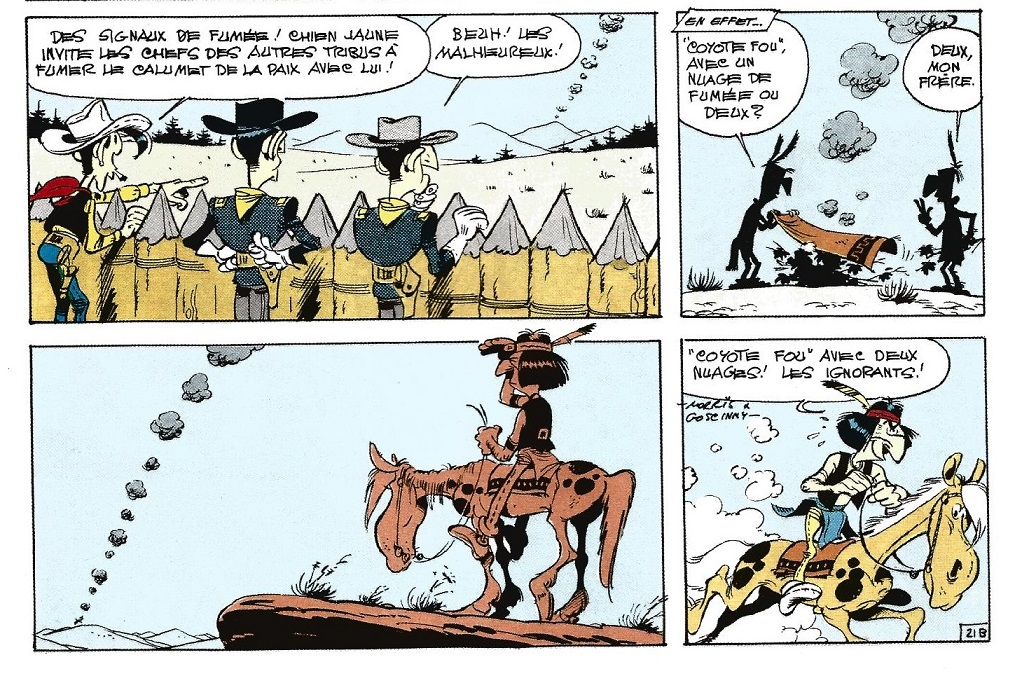
\includegraphics[scale=0.8]{LP_TraitementSignal/Codage_LuckyLuke.jpg}
\end{center}
\textcolor{green}{signal :} (ref Taillet p674) Variation temporelle ou spatiale d'une quantité physique mesurable (tension, force, lumière, ...) portant une information.\\
\textcolor{green}{Traitement du signal :} Transformation d'un signal reçu par un récepteur pour en retirer l'information transmise initialement par un émetteur. Ex : si un observateur cherche à analyser les nuages émis par le feu (\textcolor{green}{signal}), il doit se séparer de celle émise par l'environnement (\textcolor{green}{bruit}) par différents moyen (se couvrir les yeux pour se protéger du soleil). \og Se couvrir les yeux \fg~ = filtrage.

\section{Spectre et filtrage d'un signal}

\subsection{Décomposition Fourier}

Cf Cottet Chap 2 - Tout signal peut se décomposer comme une série de signaux sinusoïdaux.\\

Cf Cottet p14- Spectre d'énergie (important pour la suite car modulation DBPC problèmatique) d'un signal cf Cottet. Composante continue, fondamental, harmoniques.\\

Propriétés TF (?) et principe de la FFT sur un oscillo (pour préparer les mesures de la deuxième partie)

\subsection{Types de signaux}
Signaux analogiques vs numériques, déterministes vs aléatoires. On va se concentrer sur les signaux analogiques et déterministes.


\subsection{Réponse d'un filtre à une excitation périodique : exemple du filtre RC passe-bas}
Prendre l'exemple d'un circuit RC passe-bas (mesure sur la capa). \textcolor{blue}{Manip quantitative :} tracer le diagramme de Bode et déterminer la fréquence de coupure $f_c = \frac{1}{RC}$. Mettre en évidence le $-20\log(\omega)$. Déterminer la bande passante.

\subsection{Autres types de filtre}
\textbf{Transition :} Maintenant qu'on a décrit un signal et qu'on sait en retirer des informations, on va voir comment en envoyer un et comment le réceptionner.

\section{Modulation et démodulation en amplitude}
Fil conducteur : radio analogique. Cf cours de Jérémy.
Deux problèmes : 
\begin{itemize}
    \item \textcolor{green}{l'encombrement :} par exemple deux personnes qui parlent en même temps,
    \item dimension des antennes : longueur de l'antenne doit être de l'ordre de la longeur d'onde soit 1500km pour $f=20Hz$ et 1.5km pour $f=20000Hz$ ...
\end{itemize}

\subsection{Principe de la modulation en amplitude}
On souhaite passer à des tailles d'antennes raisonnable de l'ordre du mètre : soit $f=\frac{c}{\lambda}=30$MHz : c'est le principe de la modulation.

\textcolor{green}{Modulation :} Accrocher un signal à transmettre à une porteuse : modulation de la porteuse. Ex : pigeon voyageur (porteuse) pour faire passer une lettre (signal modulant) d'un point A à un point B\\

Pour un signal EM : 
\begin{itemize}
    \item $V_m(t)=A+B\cos(\omega_mt)$ pour la modulation (GBF Agilent à $\frac{\omega_m}{2\pi}=500$~Hz : le message à faire passer)
    \item $V_p(t) = V_0\cos(\omega_pt)$ (BGX Métrix à $\frac{\omega_p}{2\pi}=50$~kHz : le pigeon voyageur)
\end{itemize}

Faire le calcul à la sortie d'un multiplieur. Deux cas particuliers : montrer modulation DBPC ($A\neq0$) et DBPS ($A=0$).

\begin{center}
    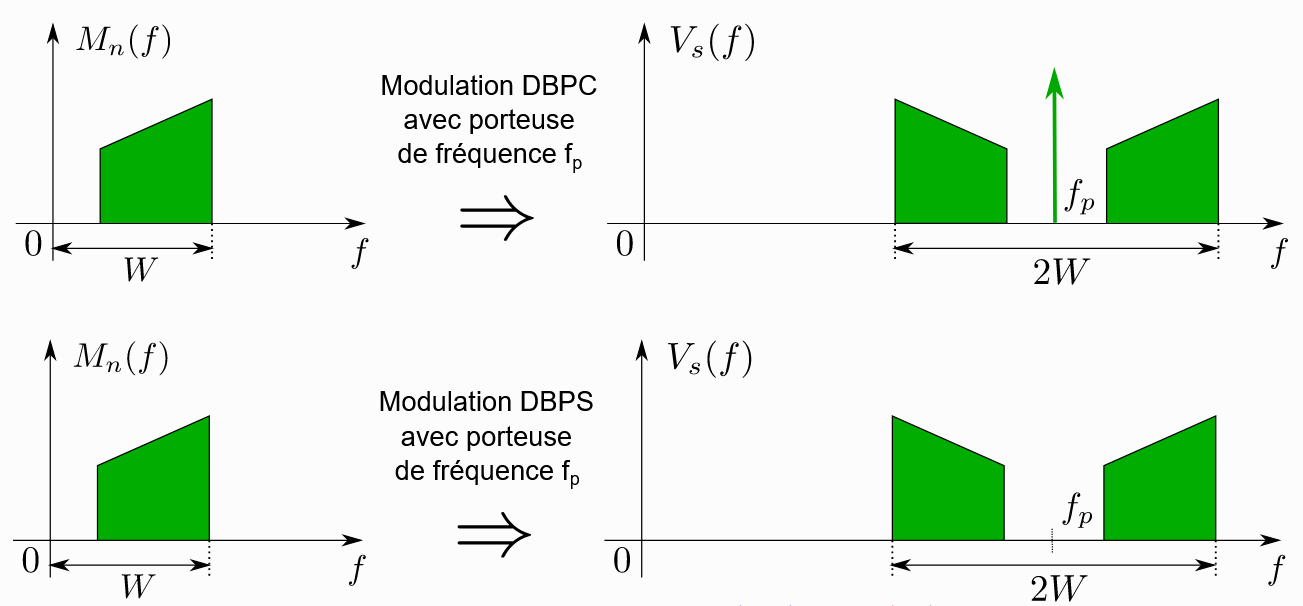
\includegraphics[scale=0.5]{LP_TraitementSignal/Modulation.png}
\end{center}



\subsection{Démodulation par détection synchrone}
Intérêt de la 
\textcolor{red}{Attention :} pour que ça puisse fonctionner, il faut que la porteuse puisse être regénérée (on peut le faire avec une boucle à vérouillage de phase cf cours Jérémy, le mentionner peut-être en conclusion de la partie).\\

\textcolor{blue}{Manip qualitative : démodulation par détection synchrone}. Le TP est bien fait, montrer le signal qu'on module, le signal après multiplication par la porteuse et le signal après le filtre passe-bas.

\textbf{Transition : }L'algorithme de FFT qu'on a largement utilisé au cours des expériences repose sur la transformée de Fourier d'un signal échantillonné (discrétisé). On va voir justement quelques avantages/inconvénients des traitements des signaux numériques.

\section{Quelques aspects du traitement des signaux numérique}

\subsection{Echantillonnage}
Voir cours de Jérémy, parler du critère de Shannon.

\subsection{Effet du fenêtrage temporel}
p190 Cottet.
\section*{Conclusion et ouverture}

Parler de la modulation en fréquence, en phase, leurs avantages. Ouvrir sur les signaux numériques. A



\end{reportBlock}
\newpage
%%%%%%%%%%%%%%%%%%%%%%%%%%%%%%%%%%%%%%%%%%%%%%%%%%%%
%%%% En-tête leçon
\begin{headerBlock}
  \chapter{Ondes progressives, ondes stationnaires.}
  \label{LP_OndesProgressives} 
\end{headerBlock}




%%%%%%%%%%%%%%%%%%%%%%%%%%%%%%%%%%%%%%%%%%%%%%%%%%%%
%%%% Références
\begin{center}
\begin{tabularx}{\textwidth}{| X | X | c | c |}
  \hline
  \rowcolor{gray!20}\multicolumn{4}{c}{Bibliographie de la leçon : } \\
  \hline 
  Titre & Auteurs & Editeur (année) & ISBN \\
  \hline
  Tout-en-un PC/PC* & M.-N. Sanz & Dunod (2022) & \\
  \hline 
   \url{http://www.etienne-thibierge.fr/agreg/ondes_poly_2015.pdf} & Ethienne Thibierge & 2015 &    \\
   \hline
   \url{http://images.math.cnrs.fr/Spectre.html\#nh7} &  San Vu Ngoc & CNRS & \\
  \hline 
  Ondes H-prépa & J-M Brébec & Hachette (2004) & \\
  \hline
  \url{https://dropsu.sorbonne-universite.fr/s/nyD9Ppz3kH6BHZE} & Clément Sayrin & & \\
\end{tabularx}
\end{center}

%%%%%%%%%%%%%%%%%%%%%%%%%%%%%%%%%%%%%%%%%%%%%%%%%%%%

%%%%%%%%%%%%%%%%%%%%%%%%%%%%%%%%%%%%%%%%%%%%%%%%%%%%
%%%% Plan
\begin{reportBlock}{Plan détaillé}

  \textbf{Niveau choisi pour la leçon :} CPGE 2ème année
  \newline
  \textbf{Prérequis} : \begin{itemize}
      \item Forces, énergie
      \item 
      \item 
  \end{itemize}
  
  \section*{Introduction}
\textcolor{green}{Slide} Quel est le point commun entre tous ces phénomènes : Olà dans un stade, effet d'une goutte qui tombe dans une flaque, un séisme, une corde soumise à des vibrations ? L'objectif de cette leçon est de donner les similitudes entre ces phénomènes et de pouvoir en retirer des caractéristiques générales.

  \section{Approches du phénomène de propagation}

  \subsection{Elongation d'une corde sans raideur}
  Voir Hprépa p30.
  \textbf{Hypothèses :} On regarde des petites perturbations de la hauteur de la corde notée $y(x,t)$. 
  Obtenir l'équation de d'Alembert unidimentionnelle.\\
  
  Donner les équations couplant $y(x,t)$ et $T(x,t)$ (p32) en disant que le phénomène de propagation est contenue dans ces équations liant vitesse transverse $\fracD{y}{t}$ et la projection de la tension suivant $\mathbf{\hat{u_y}}$.\\

  \textcolor{red}{Transition : Ce couplage entre deux grandeurs rappelle celui de la tension et du courant. On peut effectivement faire l'analogie de la propagation de U et i dans un câble coaxial avec la tension et la déformation de la corde.}

  \subsection{Analogie électrocinétique : le câble coaxial} 
  Voir HPrépa p58. \textcolor{blue}{Prendre câble coaxial, montrer l'âme et la gain et le diélectrique}. Faire le schéma d'un câble coaxial avec âme et gaine et le schéma électriue équivalent.\\
  \textbf{Hypothèses :} On ne se place plus dans l'ARQS pour le câble tout entier car on veut voir des phénomènes de propagation mais on peut le découper en tronçons dans lesquels la propagation est négligeable. \\
  
  Obtenir les équations couplées (loi des mailles et loi des n\oe uds) et obtenir l'équation de d'Alembert unidimentionnelle.\\
  \textcolor{blue}{Manip quantitative : mesure de la vitesse de propagation de i ou u dans le câble coaxial avec un câble de 100m de long. Envoyer un pulse d'impulsion 100ns, montrer le décalage sur la voie Y et mesurer ce décalage avec les curseurs. On obtient $v=\frac{2c}{3}$. On peut en déduire $n=\frac{v}{c}=\sqrt{\epsilon_r}$}.

  Définir la notion d'onde (poly Thibierge p10) : \og Une onde correspond à la propagation d’une perturbation à travers un milieu. Cette perturbation est générée par une source, qui apporte de l’énergie au milieu. L'existence de deux grandeurs couplées qui se créent l'une l'autre est à la base du phénomène de propagation.\\

  Dans le cas de la corde, une personne à mis en mouvement la corde. Dans le cas de la ligne, un expérimentateur a décidé de mettre un GBF. Dans le cas de la olà, un groupe de personne déclanche ce phénomène. Dans le cas de la goutte d'eau, un robinet qui fuit a amené de l'eau au milieu.\\

  \textcolor{green}{Slide : tableau analogie}
  
  \textcolor{red}{On a décrit le phénomène de propagation comme l'existence de deux grandeurs couplées qui se propagent dans un milieu. On va maintenant voir la forme des solutions de l'équation de d'Alembert.}
  
  

  \section{Ondes progressives}
  \subsection{Solution de l'équation de d'Alembert unidimentionnelle}
  A voir si on a le temps de la démontrer.
  
  \subsection{Interprétation}
  Voir Tec\&Doc p128 ou Dunod p806-807 et Thibierge Exos C1. Faire les dessins avec correspondance temporelle et spatiale.

  \subsection{OPPH}
  Idée : tout signal périodique peut se décomposer en série de Fourier dont chaque terme est solution de l'équation de d'Alembert. Cela est possible par la linéarité de l'équation.\\
  Obtenir la relation de dispersion. Définir vitesse de phase et vitesse de groupe. 
  
  \section{Onde stationnaire}
  On peut imaginer une onde progressive et une onde regressive qui se propagent et qui se rencontrent. 
  

  \subsection{Corde de Melde}

  \section{Conclusion}
  Conclure sur absorption, dispersion, impédance. Prendre exemple Dunod p818 en introduisant une force de frottement.


\end{reportBlock}
\newpage
%%%%%%%%%%%%%%%%%%%%%%%%%%%%%%%%%%%%%%%%%%%%%%%%%%%%
%%%% En-tête leçon
\begin{headerBlock}
  \chapter{Ondes acoustiques.}
  \label{LP_OndeAcoustique} 
\end{headerBlock}




%%%%%%%%%%%%%%%%%%%%%%%%%%%%%%%%%%%%%%%%%%%%%%%%%%%%
%%%% Références
\begin{center}
\begin{tabularx}{\textwidth}{| X | X | c | c |}
  \hline
  \rowcolor{gray!20}\multicolumn{4}{c}{Bibliographie de la leçon : } \\
  \hline 
  Titre & Auteurs & Editeur (année) & ISBN \\
  \hline
  Tout-en-un PC/PC* & M.-N. Sanz & Dunod (2022) & \\
  \hline 
   \url{http://www.etienne-thibierge.fr/agreg/ondes_poly_2015.pdf} & Ethienne Thibierge & 2015 &  \\
  \hline 
  Ondes H-prépa & J-M Brébec & Hachette (2004) & \\
  \hline
  \url{https://dropsu.sorbonne-universite.fr/s/nyD9Ppz3kH6BHZE} & Clément Sayrin & & \\
  \hline
  Ondes acoustiques & A. Chaigne & Ecole Polytechnique (2011) & \\
  \hline
\end{tabularx}
\end{center}

%%%%%%%%%%%%%%%%%%%%%%%%%%%%%%%%%%%%%%%%%%%%%%%%%%%%

%%%%%%%%%%%%%%%%%%%%%%%%%%%%%%%%%%%%%%%%%%%%%%%%%%%%
%%%% Plan
\begin{reportBlock}{Plan détaillé}

  \textbf{Niveau choisi pour la leçon :} 
  \newline
  \textbf{Prérequis} : \begin{itemize}
      \item 
      \item 
      \item 
  \end{itemize}
  
  \section*{Introduction}

  \section{}

  \subsection{}   

  \section{}

  \subsection{}
  
  \section{}
  


\end{reportBlock}
\newpage
%%%%%%%%%%%%%%%%%%%%%%%%%%%%%%%%%%%%%%%%%%%%%%%%%%%%
%%%% En-tête leçon
\begin{headerBlock}
  \chapter{Propagation guidée des ondes.}
  \label{LP_PropagationGuidee} 
\end{headerBlock}




%%%%%%%%%%%%%%%%%%%%%%%%%%%%%%%%%%%%%%%%%%%%%%%%%%%%
%%%% Références
\begin{center}
\begin{tabularx}{\textwidth}{| X | X | c | c |}
  \hline
  \rowcolor{gray!20}\multicolumn{4}{c}{Bibliographie de la leçon : } \\
  \hline 
  Titre & Auteurs & Editeur (année) & ISBN \\
  \hline
   Electromagnétisme & Pérez & Dunod & \\
  \hline 
   \url{http://www.etienne-thibierge.fr/agreg/ondes_poly_2015.pdf} & Etienne Thibierge & &    \\
  \hline 
   &  & &    \\
  \hline 
\end{tabularx}
\end{center}

%%%%%%%%%%%%%%%%%%%%%%%%%%%%%%%%%%%%%%%%%%%%%%%%%%%%

%%%%%%%%%%%%%%%%%%%%%%%%%%%%%%%%%%%%%%%%%%%%%%%%%%%%
%%%% Plan
\begin{reportBlock}{Plan détaillé}

  \textbf{Niveau choisi pour la leçon :}
  \newline
  \textbf{Prérequis} : \begin{itemize}
      \item propagation des ondes EM dans le vide, équations de Maxwell,
      %\item Impédance d'un milieu
      \item optique ondulatoire (conditions d'interférences)
      \item optique géométrique : théorème de Malus, principe du retour inverse de la lumière
  \end{itemize}

  \textbf{Déroulé détaillé de la leçon: }  
  
  \section*{Introduction}
  Pour transmettre une onde sphérique (sonore ou électromagnétique) à partir d'une source, on voit qu'il y a un problème car l'amplitude de l'onde varie en $1/r$ et la densité locale d'énergie de l'onde varie en $1/r^2$ par conservation de l'énergie. Si on veut transmettre une information, il faut donc soit une très grande puissance à l'entrée (dangereux et pas spécialement possible techniquement), soit être plus malin et guider l'onde jusqu'au récepteur. On va cependant voir qu'il existe quelques contraintes.
  \textcolor{blue}{Expérience qualitative : deux émetteurs piézo avec ou sans tube.}

  %\section{Propagation (partie qui peut sauter}
  %\subsection{Champs couplés}
  %\subsection{Impédance caractéristique}
  %Montrer ce qui se passe si $Z=+\infty$, $Z=0$ et $Z=Z_c$.

  %\section{Ondes TEM dans un câble coaxial}
  
  %\subsection{Equation des télégraphistes}
  \section{Phénoménologie du guidage}
  Ne pas passer trop de temps sur cette partie ($\sim$10min). Faire le dessin. On prend l'approche phénoménlogique du guidage d'ondes lumineuses dans la fibre optique.
  
  \subsection{Modèle de la fibre optique}
  
  Faire le schéma de la fibre optique tel que dans le poly de Thibierge. On regarde la propagation d'une onde plane monochromatique de longeur d'onde dans le vide $\lambda$\\
  \textcolor{red}{Condition de guidage :} interférences constructives entre deux réflexions sucessives \textit{i.e.} que leur déphasage soit un multiple de $2\pi$.\\
  
  \subsection{Caractéristiques du guidage}
  Après construction de $S_0$, $S_1$ et $S_2$, on obtient le déphasage entre l'onde issue de $S_0$ et celle issue de $S_2$ :
  \begin{equation}
      \Delta\phi = \frac{2\pi}{n_2\lambda}n_2S_2B - \frac{2\pi}{n_1\lambda}n_1S_0B = \frac{2\pi}{\lambda}S_2H
  \end{equation}
  d'après le principe de retour inverse + théorème de Malus. Comme $\sin{\theta}=\frac{S_2H}{2a}$ : 
  \begin{equation}
      \sin(\theta_p) = \frac{p\lambda}{2a}
  \end{equation}
  Les angles d'incidence qui permettent la propagation dans la fibre prennent des valeurs discrètes ! \textbf{$p$ désigne un mode de propagation dans la fibre}.\\

  Tous les modes ne peuvent pas se propager :
  \begin{equation}
      sin(\theta_p)\leq 1 \Rightarrow \omega \geq p\frac{\pi c}{a} = \omega_{c,p}
  \end{equation}
  \textbf{Une pulsation de coupure basse fréquence est associée à chaque mode en dessous de laquelle il n'y a pas guidage}. \textbf{On peut donc guider uniquement des ondes dont les longueurs d'ondes sont inférieures à $2a\sim10^{-3}m$} : optique, infrarouge.\\
  Application numérique : pour $\lambda=500nm$ et $a=1mm$, on peut avoir $p=4000$ modes de propagation dans la fibre.\\

  Parler de dispersion intermodale et intramodale ? En parler après si on a le temps.\\

  \textcolor{red}{Pour les ondes de plus basses fréuences, on est obligé d'utiliser d'autres systèmes : fil conducteur pour les ondes BF ($<1$MHz), câbles coaxiaux pour les ondes HF ($<1$GHz). Pour les ondes centimétriques, on a besoin de guide d'ondes creux dont on va maintenant détailler la physique plus quantitativement que pour les ondes lumineuses.}
  
  \section{Propagation d'une onde centimétrique dans un guide}
   Dans les câbles coaxiaux, il y a une importante atténuation des signaux pour les fréquences supérieures à 1 GHz. On utilise pour ces fréquences d'autres supports. On va s'intéresser dans cette partie à la possibilité qu'une onde électromagnétique puisse se propager dans un guide plan. 
  \subsection{Modélisation idéalisée du guide plan}
  Faire le schéma. Voici les hypothèses :
  \begin{itemize}
      \item L'étude de la propagation des ondes dans les milieux conducteurs montre qu'il existe une onde evanescente qui transporte de l'énergie hors du guide. Ici on va supposer les \textbf{conducteurs parfaits} pour supprimer les pertes et simplifier les calculs,
      \item Le milieu entre les plaques est de l'air qu'on va idéaliser à du vide pour enlever les effets de dispersion qui n'est pas propre au guidage.
  \end{itemize}
  L'équation de propagation est celle des ondes dans le vide c'est-à-dire une équation de d'Alembert :
  \begin{align}
      \mathbf{\Delta E} &= \frac{1}{c^2}\partialD{\mathbf{E}}{t} \\
      \mathbf{\Delta B} &= \frac{1}{c^2}\partialD{\mathbf{B}}{t}
  \end{align}
  En revanche, du fait de la présence du guide, les champs $\mathbf{E}$ et $\mathbf{B}$ doivent satisfaire les conditions aux limites à savoir la continuité de la composante tangentielle de $\mathbf{E}$ et la composante normale de $\mathbf{B}$ qui s'annulent aux deux faces :
  \begin{align}
      E_z(x=0)&=E_z(x=a)=0 & E_y(x=0)&=E_y(x=a)\\
      B_x(x=0)&=0 & B_x(x=a)&=0
  \end{align}
  On va chercher des solutions qui se propagent dans la direction z du guide. Comme il y a également invariance par translation suivant $\mathbf{\hat{u_z}}$, on peut écrire les ondes comme :
  \begin{align}
      \mathbf{E} &= \mathbf{E_m}(x)e^{i(\omega t - k_zz)}\\
      \mathbf{B} &= \mathbf{B_m}(x)e^{i(\omega t - k_zz)}
  \end{align}
  Remarquons qu'ici on n'a pas la structure d'onde plane car il y a une dépendance de l'amplitude de l'onde EM en x. On définit alors :
  \begin{equation}
      \lambda_g = \frac{2\pi}{k_z}
  \end{equation}
  la longueur d'onde de l'onde guidée.\\
  On va également définir :
  \begin{itemize}
      \item les ondes transverses électriques TE qui sont reliées aux composantes $E_z$ et $E_y$ de l'onde dans le guide,
      \item les ondes transverses magnétiques reliées aux composantes $B_y$ et $B_z$ de l'onde dans le guide
  \end{itemize}
  Ce sont les équations de Maxwell-Faraday et Maxwell-Ampère qui nous permettent de définir ces deux groupes d'ondes transverses. La linéarité des équations permettent d'étudier séparément ces deux groupes et d'obtenir l'ensemble des solutions par combinaison linéaire.\\

  \textcolor{red}{On va regarder uniquement les ondes TE.}
  
  \subsection{Relation de dispersion des ondes TE dans le guide}
  On cherche les solutions $\mathbf{E}$ sous la forme :
  \begin{equation}
      \mathbf{E} = (E_x(x)\mathbf{\hat{e}_x}+E_y(x)\mathbf{\hat{e}_y})e^{i(\omega t - k_zz)}
  \end{equation}
  Comme $\grad\cdot\mathbf{E} = \partialD{E_z}{z}=ik_zE_z=0$ donc $E_z=0$. En injectant cette solution dans l'équation de d'Alembert :
  \begin{align}
      \frac{d^2E_y}{dx^2} + \frac{d^2E_y}{dz^2} &= \frac{1}{c^2}\partialD{^2E_z}{t^2} \\
       \frac{d^2E_y(x)}{dx^2} + (k^2-k_z^2)E_y(x) &=0
  \end{align}
  avec les conditions $E_y(0)=E_y(a)=0$. Il y a trois cas de figure :
  \begin{enumerate}
      \item Si $k^2-k_z^2<0$, on peut montrer qu'il n'y a pas de solutions qui se propagent avec les CL,
      \item Si $k^2-k_z^2=0$, on a une solution affine qui est nulle avec les CL,
      \item Si $k^2-k_z^2=k_x^2>0$, on la possibilité d'une solution qui se propage dans le guide.
  \end{enumerate}

  La solution s'écrit : 
  \begin{equation}
      E_y = Ae^{ik_xx}+Be^{-ik_xx}
  \end{equation}
  Les CL donnent :
  \begin{align}
      E_y(x=0)=0 &\Rightarrow A=-B \\
      E_y(x=a)=0 &\Rightarrow k_x=p\frac{\pi}{a}
  \end{align}
  On a alors des modes de propagation des ondes TE comme pour la fibre. On notera ces mode TE$_{p}$. On a une relation de dispersion non linéaire entre $k_z=\frac{2\pi}{\lambda_g}$ et $\omega=2\pi\frac{c}{\lambda_0}$ qu'on peut écrire comme :
  \begin{equation}
      \lambda_g^2 = \frac{\lambda_0^2}{1-\left(\frac{\lambda_0}{\lambda_c}\right)^2}
  \end{equation}
  On a ici introduit une \textbf{fréquence de coupure} $\lambda_c=\frac{2a}{p}$. Si on envoie une onde de longueur d'onde $\lambda$, elle peut se propager dans des modes TE$_p$ si $\lambda_p\geq\lambda_c$. Le guide se comporte comme un filtre passe-haut.\\
  
  Si il n'y a que le mode TE$_1$ qui peut se propager, \textcolor{green}{le guide est monomode}. Si l'onde peu se propager dans plusieurs modes TE, le guide est dit \textcolor{green}{multimode}. \\
  
  \textbf{Remarque :} le milieu est dispersif non par rapport à sa nature (on a supposé que c'était du vide) mais par rapport à la géométrie du guide.\\

  \textcolor{red}{Transition : je vous propose de vérifier cette relation dans le cadre du guide d'onde rectangulaire.}

  \subsection{Relation de dispersion du mode TE$_1$ dans le guide rectangulaire}
  \textcolor{green}{Sur slide : }Pour être rigoureux, on peut montrer qu'il y a des modes TE$_{p,q}$ qui peuvent se propager dans le guide du fait de deux interfaces. La relation de dispersion du guide rectangulaire de côté $a$ et $b$ pour ces modes est :
  \begin{equation}
      k^2 = k_z^2 + p^2\frac{\pi^2}{a^2}+q^2\frac{\pi^2}{b^2}
  \end{equation}
  Ce guide est monomode pour des pulsations ($a=22.860\pm0.046$~mm et $b=10$~mm :
  \begin{align}
      \left(\frac{\pi^2}{a^2}\right) &\leq \frac{\omega^2}{c^2} \leq \left(\frac{\pi^2}{a^2}\right) + \left(\frac{\pi^2}{b^2}\right) \\
      6.56~GHz &\leq f \leq 16.4GHz 
  \end{align}
  Comme on dispose d'une diode Gunn pouvant produire des ondes allant de $8.2$~GHz à $10$~GHz, on ne peut propager que le mode TE$_{10}$ dont la relation de dispersion est donnée par l'équation (15.17).\\
  
  \textcolor{blue}{Expérience quantitative :} Vérification de la relation de dispersion dans un guide et mesure de la fréquence de propagation dans un guide d'onde (TP Onde 2).

  \subsection{Vitesse de phase et vitesse de groupe}
  Pour $p=1$ :
  \begin{align}
      v_{\phi} &= \frac{\omega}{k_z} = \frac{c}{1-\frac{\lambda_0^2}{\lambda_c^2}} \\
  \end{align}
  \textcolor{red}{Transition : On a vu la relation de dispersion des ondes dans le guide, on va voir plus en détail l'aspect expérimental du guide d'onde.}

  \section{Aspect expérimental du guide d'onde}
  Si on a le temps : parler des pertes, du ROS, de l'abbaque de Smith.
  
  \section*{Conclusion}

  

  
  

\end{reportBlock}
\newpage
%%%%%%%%%%%%%%%%%%%%%%%%%%%%%%%%%%%%%%%%%%%%%%%%%%%%
%%%% En-tête leçon
\begin{headerBlock}
  \chapter{Microscopies optiques}
  \label{LP_Microscopie} 
\end{headerBlock}




%%%%%%%%%%%%%%%%%%%%%%%%%%%%%%%%%%%%%%%%%%%%%%%%%%%%
%%%% Références
\begin{center}
\begin{tabularx}{\textwidth}{| X | X | c | c |}
  \hline
  \rowcolor{gray!20}\multicolumn{4}{c}{Bibliographie de la leçon : } \\
  \hline 
  Titre & Auteurs & Editeur (année) & ISBN \\
  \hline
  Slide de cours & Agnès Maître & Site Montrouge & \\
  \hline 
  \url{http://ressources.agreg.phys.ens.fr/media/ressources/RessourceFichiers/11-Maxime_Dahan_-_Microscopie_pour_la_biologie.pdf} & M. Dahan & & \\
  \hline
  \url{https://www.microscopyu.com/} & Nikon & &    \\
  \hline 
  Optique & Eugène Hecht & Pearson &   \\
  \hline 
  Optique & Sylvain Houard & de Boeck & \\
  \hline
\end{tabularx}
\end{center}

%%%%%%%%%%%%%%%%%%%%%%%%%%%%%%%%%%%%%%%%%%%%%%%%%%%%

%%%%%%%%%%%%%%%%%%%%%%%%%%%%%%%%%%%%%%%%%%%%%%%%%%%%
%%%% Plan
\begin{reportBlock}{Plan détaillé}

  \textbf{Niveau choisi pour la leçon :} 
  \newline
  \textbf{Prérequis} : \begin{itemize}
      \item 
  \end{itemize}

  \textbf{Déroulé détaillé de la leçon: }  
  
  \section*{Introduction}


  \section{Le microscope \og d'autrefois \fg }

  \subsection{Présentation du dispositif}
  Faire le schéma du microscope : objectif, oculaire, image secondaire, etc ...

  \subsection{Propriétés}
  Faire le calcul de grossissement commercial $G_{com}=\frac{\alpha'}{\alpha}$\\
  Parler d'ouverture numérique, profondeur de champ, système d'éclairement, aberrations (chromatiques, géométriques)
  
  \subsection{Mesure du grossissement}
 
  \textcolor{blue}{Expérience quantitative :} Faire l'image d'une grille par un microscope optique, remonter au grossissement et comparer par rapport à la valeur de référence.

  \subsection{Limitations}
  Parler de : 
  \begin{itemize}
      \item conditions d'éclairement (éclairage Köhler
      \item résolution optique (ouverture numérique, diffraction, aberrations) 
      \item contraste
      \item microscopie plein champ/ point par point
  \end{itemize}


\textbf{Transition :} on va voir comment améliorer le microscope classique

\section{Microscopie confocal}

\section*{Ouverture}
Microscopie par effet tunnel

\end{reportBlock}
\newpage
%%%%%%%%%%%%%%%%%%%%%%%%%%%%%%%%%%%%%%%%%%%%%%%%%%%%
%%%% En-tête leçon
\begin{headerBlock}
  \chapter{Interférences à deux ondes en optique}
    \label{LP_InterferencesDeuxOndes}
\end{headerBlock}

%%%%%%%%%%%%%%%%%%%%%%%%%%%%%%%%%%%%%%%%%%%%%%%%%%%%
%%%% Références
\begin{center}
\begin{tabularx}{\textwidth}{| X | X | c | c |}
  \hline
  \rowcolor{gray!20}\multicolumn{4}{c}{Bibliographie de la leçon : } \\
  \hline 
  Titre & Auteurs & Editeur (année) & ISBN \\
  \hline
Physique Spé MP-MP* & Olivier, Gié, Sarmant & Tec \& Doc & \\
  \hline 
  Sextant &  & Hermann &  \\
  \hline 
   Tout-en-un, MP & M.-N. Sanz. & Dunod &  \\
   \hline
   Optique & Eugene HECHT & Pearson (2005) & \\
   \hline
   Optique & S. Houard & de Boeck & \\
   \hline
\end{tabularx}
\end{center}

%%%%%%%%%%%%%%%%%%%%%%%%%%%%%%%%%%%%%%%%%%%%%%%%%%%%
\begin{reportBlock}{Plan détaillé}
  \textbf{Niveau choisi pour la leçon :} CPGE
  \newline
  \textbf{Prérequis : }Modèle scalaire d'une onde, chemin optique, différence de marche, intensité lumineuse, formules trigonométriques
  \newline
  
  \textbf{Déroulé détaillé de la leçon: } \newline
\textcolor{green}{Manip introductive :} si on superpose deux lasers, il ne se passe rien. Si on les fait passer à travers un dispositif qui élargit le faisceau + une fente source + une bifente : on voit une figure d'interférence.
  \section{Interférences à deux ondes}
  \textcolor{red}{Définition :} phénomène ondulatoire qui résulte d'une interaction entre deux ondes (lumineuses) qui produit une intensité totale qui diffère de la somme des intensités individuelles.
  \subsection{Superposition de deux ondes}
  On considère deux sources ponctuelles $S_1$ et $S_2$ et des amplitudes vibratoires $a_i(M,t)=A_i\cos\left(\omega_it-\phi_{S_i} - \frac{2\pi[S_iM]}{\lambda_0i}\right)$. L'amplitude totale est : $a(M,t)=a_1(M,t)+a_2(M,t)$. L'intensité est : $I(M,t) = <a^2(M,t)>$.\\

  En développant, on obtient :
  \begin{equation}
      I = I_1 + I_2 + I_{1,2}
  \end{equation}
  avec $I_{1,2} = 2A_1A_2\cos\left(\omega_1t-\phi_1(M)\right)\cos\left(\omega_2t-\phi_2(M)\right)$

  \subsection{Conditions d'interférence, notion de cohérence}
  \begin{itemize}
      \item $I_{1,2}\neq$, dans ce cas on dit que les ondes sont cohérentes,
      \item si $\omega_1\neq\omega_2$, $I_{1,2}=0$
  \end{itemize}

  \underline{\textcolor{red}{Condition 1 :}} deux ondes de pulsations différentes sont incohérentes.\\

  Présentation du modèle du train d'onde : paquet d'onde séparés par un temps $\tau$. Comme $\phi_{S1}$ et $\phi_{S2}$ varient aléatoirement, on obtient $I_{1,2}$ non nulles sur le détecteur si :\\
  \underline{\textcolor{red}{Condition 2 :}} Il faut que les deux ondes soient issus du même train d'onde. \\

  On obtient alors la formule de Fresnel :
  \begin{equation}
      I = I_1 + I_2 + 2\sqrt{I_1I_2}\cos{\Delta\phi(M)}  \end{equation}
      où $\Delta\phi(M) = \frac{2\pi([S_2M]-[S_1M])}{\lambda_0}$

\section{Exemple d'interféromètre : les trous d'Young}
Cf photo.

\begin{equation}
    I = 2I_0\left[1+\cos\left(\frac{2\pi ax}{D}\right)\right]
\end{equation}
Succesion de franges brillantes et de franges sombres. La distance entre deux franges brillantes est appelée \textcolor{red}{interfrange} notée $i$ qui vaut ici : $i=\frac{\lambda_0D}{a}$.\\
\textcolor{green}{Manipulation 2 (quantitative) :} Mesure de l'interfrange de la figure d'interférences pour en déduire $a$. On mesure $a=0.16\pm0.04$mm à comparer avec la valeur $a_{fabricant}=0.2$mm.

\section{Notion de cohérence spatiale}
Effet de la largeur de la source en reprenant le problème avec deux sources séparées par une distance $b$. On obtient à l'aide des formules obtenues dans la partie précédente : 
\begin{equation}
    I_{tot} = 4I_0\left[1+\cos\left(\frac{\pi ab}{\lambda D}\right)\cos\left(\frac{2\pi a x}{\lambda D}+\frac{2\pi a b}{\lambda D}\right)\right]
\end{equation}
\section{Conclusion}
Ouverture sur les dispositifs à division du front d'onde et division d'amplitude.
\end{reportBlock}


\begin{reportBlock}{Questions posées par l’enseignant (avec réponses)}
   \textbf{C : D'autres phénomènes d'interférences autres que lumineuses ?}  \textcolor{purple}{Oui, exemple de la cuve à onde.} Qu'est-ce qui fait la spécificité des interférences des ondes lumineuses ? \textcolor{purple}{On peut faire des mesures super précises.}\\
   \textbf{C : Conditions de cohérence pour l'eau ?}  \textcolor{purple}{On somme directement les amplitudes, il n'y a pas de notion de cohérence pour une onde mécanique.}\\
   \textbf{C : Dépendence de la durée d'intégration ? Odg temps de réponse d'un détecteur ?}  \textcolor{purple}{Période de la lumière  : $10^{-15}$s, \oe uil : $10^{-2}$s,  photorésistance $10^{-2}$s, photodiode (standard): $10^{-6}$s, thermopile : $1$s}\\
   \textbf{C : lien entre intensité $I$ et éclairement $\epsilon$ ?}  \textcolor{purple}{On a $\epsilon = KI = K<s^2(M,t)>$, où $<...>$ représente la valeur moyenne temporelle, K est une constante qui dépend du détecteur et $s(M,t)$ représente une composante du champ électrique de la lumière par rapport à un axe perpendiculaire à sa direction de propagation. L'éclairement est la puissance surfacique moyenne de l'onde lumineuse (autrement dit la valeur moyenne temporelle du vecteur de Poynting).}\\
   \textbf{C : Pourquoi il faut un vide entre deux trains d'ondes ?}  \textcolor{purple}{Lié à la désexcitation de l'atome, la durée de vie d'un niveau d'énergie.} Un train d'onde c'est un photon du coup ? \textcolor{purple}{C'est l'aspect ondulatoire du photon.}\\
   \textbf{C : C'est quoi la cause de l'incohérence spatiale ?} \textcolor{purple}{Emission de trains d'onde de phase à l'origine aléatoire suivant l'atome émetteur.}\\

   \textbf{C : Différences/avantages interférométrie à division d'amplitude/ division du front d'onde ?} \textcolor{purple}{Division du front d'onde : on fait interférer de la lumière provenant de deux sources différentes. Les interférences ne sont pas localisées mais il y a un problème de brouillage du fait de la cohérence spatiale des sources. Division d'amplitude : on fait interférer de la lumière provenant d'un même faisceau incident dont on a séparé en deux (au moins) l'amplitude. Il n'y a pas de problème lié à la cohérence spatiale de la source mais le prix à payer est la localisation des interférences (à l'infini pour une lame d'air, à distance finie pour un coin d'air). L'avantage est de pouvoir utiliser des sources de lumière très étendues, on gagne en luminosité.}\\

   \textbf{C : Stratégies à mettre en \oe uvre pour éviter $20\%$ d'erreur sur les mesures ?} \textcolor{purple}{Caméra CCD, mettre une lentille pour agrandir l'image} Ca change quoi avec une lentille ? \textcolor{purple}{On remplace $D$ par $f'$ dans la formule de $I_{tot}$.} C'est mieux du coup ? \textcolor{purple}{On peut mesurer $f'$ de façon assez précise} Quoi d'autre ? \textcolor{purple}{Pied à coulisse, banc optique, ...}\\
   
\end{reportBlock}

\newpage
%%%%%%%%%%%%%%%%%%%%%%%%%%%%%%%%%%%%%%%%%%%%%%%%%%%%
%%%% En-tête leçon
\begin{headerBlock}
  \chapter{Interférométrie à division d'amplitude}    \label{LP_DivisionAmplitude}
\end{headerBlock}



%%%%%%%%%%%%%%%%%%%%%%%%%%%%%%%%%%%%%%%%%%%%%%%%%%%%
%%%% Références
\begin{center}
\begin{tabularx}{\textwidth}{| X | X | c | c |}
  \hline
  \rowcolor{gray!20}\multicolumn{4}{c}{Bibliographie de la leçon : } \\
  \hline 
  Titre & Auteurs & Editeur (année) & ISBN \\
  \hline
   Optique physique et électronique  & Daniel Mauras & Presse Universitaire de France (2004) &  \\
  \hline 
   Optique Physique & Richard Taillet & de boeck (2015) & 953-087864-7\\
  \hline 
   Optique & Sylvain Houard & de boeck (2014) & \\
  \hline 
  Optique et phyique ondulatoire & Bertin Faroux Renault & Dunod (1986) & \\
  \hline
\end{tabularx}
\end{center}


%%%%%%%%%%%%%%%%%%%%%%%%%%%%%%%%%%%%%%%%%%%%%%%%%%%%
%%%% Plan
\begin{reportBlock}{Plan détaillé}
  \textbf{Niveau choisi pour la leçon :} Licence 3
  \newline
  \textbf{Prérequis :} Optique Géométrique, Interférences à deux ondes, Interférences à division du front d'onde, cohérence temporelle/cohérence spatiale
  \newline
  
  \textbf{Déroulé détaillé de la leçon: }\newline
  \section*{Introduction : interférences à division du front d'onde}
  Interférences sont beaucoup utilisées en physique et même dans la vie de tous les jours : exemple du casque anti-bruit qui fait interférer les ondes sonores de l'extérieur avec celles du son dans le casque audio.\\
  Dans la suite, on s'intéresse aux interférences à deux ondes lumineuses.\\
  Retour sur les fentes d'Young (\textcolor{green}{slide 1}). Avec un éclairement des fentes par une source ponctuelle, on observe des franges d'interférences non localisées sur un écran.\\
  \textbf{Problème :} (\textcolor{green}{slide 2}) quand on augmente la taille de la source, on observe un brouillage de la figure d'interférences et donc une perte de contraste : problème de cohérence spatiale de la source.\\
  On va voir que l'interférométrie à division d'amplitude permet de s'affranchir de se problème.
  Annonce du plan : 
  \begin{itemize}
      \item Division d'amplitude
      \item Un exemple d'interféromètre à division d'amplitude
      \item Une application pratique de la division d'amplitude
  \end{itemize}
  
  \section{Division d'amplitude}
  \subsection{Théorème de localisation}
  Considérons un système interféromètrique éclairé par une source monochromatique étendue tel que représenté sur la Figure \ref{fig:localisation}. On souhaite qu'au point M, les intensités lumineuses provenant de S et S' qui s'ajoutent ne produisent pas de brouillage. Autrement dit, nous avons la condition de non-brouillage au point M suivante :\newline
  \textcolor{red}{Condition de non-brouillage :} $\Delta(M)=\delta(S',M)-\delta(S,M)=0$ \newline
  On montre (dans D. Mauras p. 159) que :
  \begin{equation}
      -n(\mathbf{u}_2-\mathbf{u}_1)\cdot\mathbf{SS'}=0
  \end{equation}
  Cette équation nous permet de distinguer deux cas :
  \begin{itemize}
      \item $\mathbf{u}_2\ne\mathbf{u}_1$ : c'est une contrainte sur la source, les rayons qui interfèrent en M ne sont pas issus du même rayon incident. C'est le cas des interféromètres à \textbf{division du front d'onde}.
      \item $\mathbf{u}_2=\mathbf{u}_1$ : c'est une contrainte sur l'interféromètre. Les rayons qui interfèrent sont issus du même rayon incident. Le système optique doit contenir une lame séparatrice qui divise en deux un rayon incident puis fait interférer les deux rayons ainsi créés: c'est \textbf{la division d'amplitude}.
  \end{itemize}
  \textcolor{red}{Théorème de localisation :} (\textcolor{green}{Slide 3}) Seuls les dispositifs à division d'amplitude peuvent donner des interférences contrastées produites par des sources arbitrairement larges. Ces interférences sont alors \textbf{localisées} au voisinage des points d'intersection des couples de rayons lumineux issus du même rayon incident.
  
  \subsection{Lame d'air}
  Un exemple simple d'interféromètre à division d'amplitude est celui de la lame d'air. On peut montrer que la différence de marche entre deux rayons lumineux sortant de la lame d'air est donné par :
  \begin{equation}
      \delta(M) = 2ne\cos{i}
  \end{equation}
  avec $e$ l'épaisseur de la lame d'air et $i$ l'angle d'incidence du rayon lumineux provenant de la source S.
  On peut faire quelques remarques : 
  \begin{itemize}
      \item Les interférences sont localisées à l'infini, il faut donc une lentille convergente et un écran placé dans le plan focal image de cette dernière pour observer la figure d'interférences,
      \item Pour une même épaisseur $e$, l'intensité lumineuse ne dépend que de $i$ : on observe des franges circulaires dites \textbf{d'égales inclinaison} qu'on comprend bien en analysant les hyperboloïdes d'interférences (\textcolor{green}{slide 4}),
      \item Pour une source étendue, les franges sont plus brillantes.
  \end{itemize}
  On va voir à présent un système interférométrique réalisant effectivement la lame d'air : il s'agit de l'interféromètre de Michelson.
  
  \section{Interféromètre de Michelson}
  Rappel historique : Expérience de Michelson et Morlay au 19$^{e}$ qui démontre que la vitesse de la lumière est la même dans toutes les directions. Prix Nobel de Physique décerné à Albert Michelson en 1907.
  \subsection{Présentation du montage en configuration lame d'air}
  Le schéma de principe est présenté (\textcolor{green}{slide 5}). Schéma équivalent au tableau tel que représenté sur la Figure \ref{fig:Michelson}.
  Le Michelson n'est certes pas sensible à la cohérence spatiale de la source mais est sensible à sa cohérence temporelle : $\delta(M)\sim 2e<L_c=c\tau_c=c/\Delta\nu=\Delta\lambda/\lambda^2 $. En odg : 
  \begin{itemize}
      \item laser He-Ne à $\Delta\nu=10MHz$, $L_c\sim 30$m
      \item lumière blanche, $L_c\sim 1\mu$m
  \end{itemize}
  Ainsi pour régler le Michelson, on commence par utiliser un laser qui est une source spatialement et temporellement cohérente. Si on souhaite changer de source temporellement moins cohérente que le laser, on se met au contact optique ($e=0$) en utlisant a propriété suivante :on peut montrer que le rayon des anneaux est proportionnel à $1/\sqrt{e}$, ainsi si $e$ diminue, les anneaux s'aggrandissent et rentrent vers leur centre.\newline
  $\rightarrow$ \textcolor{blue}{observation de la figure d'interférence d'un Michelson éclairé par lampe à vapeur de sodium. On voit les anneaux avec une lentille de $f'=20$cm (faible luminosité de la source et salle assez éclairée, utiliser un condenseur à la sortie de la source pour maximiser l'éclairement sur les miroirs) et on peut repérer le contact optique. On observe également un brouillage des franges pour certaines positions du miroir (M1) car doublet du sodium.}\newline
  On va mesurer l'écart en longueur d'onde de ce doublet.
  
  \subsection{Mesure interféromètrique du doublet du sodium}
  On rappelle la formule de l'éclairement pour deux sources lumineuses de longueur d'onde différente (\textcolor{green}{slide 6}). L'écart $\Delta e$ entre deux anticoïncidences est donné par :
  \begin{equation}
      \Delta e = \frac{\bar{{\lambda}}}{2\Delta\lambda^2}
  \end{equation}
  avec $\Delta\lambda =|\lambda_2-\lambda_1|$ et $\bar{{\lambda}}=\frac{\lambda_1+\lambda_2}{2}$.\newline
  $\rightarrow$ \textcolor{blue}{S'éloigner du contact optique de ma nière à pouvoir visualiser 5 ou 6 anticoïncidences. Mesurer $\Delta e$, déterminer $\Delta\lambda$ avec son incertitude et comparer à la valeur tabulée $\Delta\lambda=0,597$nm (Encyclopedia Brittanica).}\\
  Grâce au Michelson, on est capable de faire des mesures interféromètriques très précises (inférieures au nm !).
  
  \section*{Conclusion}
  Présentation de la tomographie en cohérence optique (\textcolor{green}{Slide 7}). Voir R. Taillet.\\
  Ouverture sur le Fabry-Pérot avec la visualisation des anneaux du doublet du sodium obtenues par Fabry-Pérot (contraste des systèmes d'anneaux de $\lambda_1$ et $\lambda_2$) (\textcolor{green}{Slide 8})
\end{reportBlock}

\clearpage
  \begin{figure}[!htbp]
  \centering
  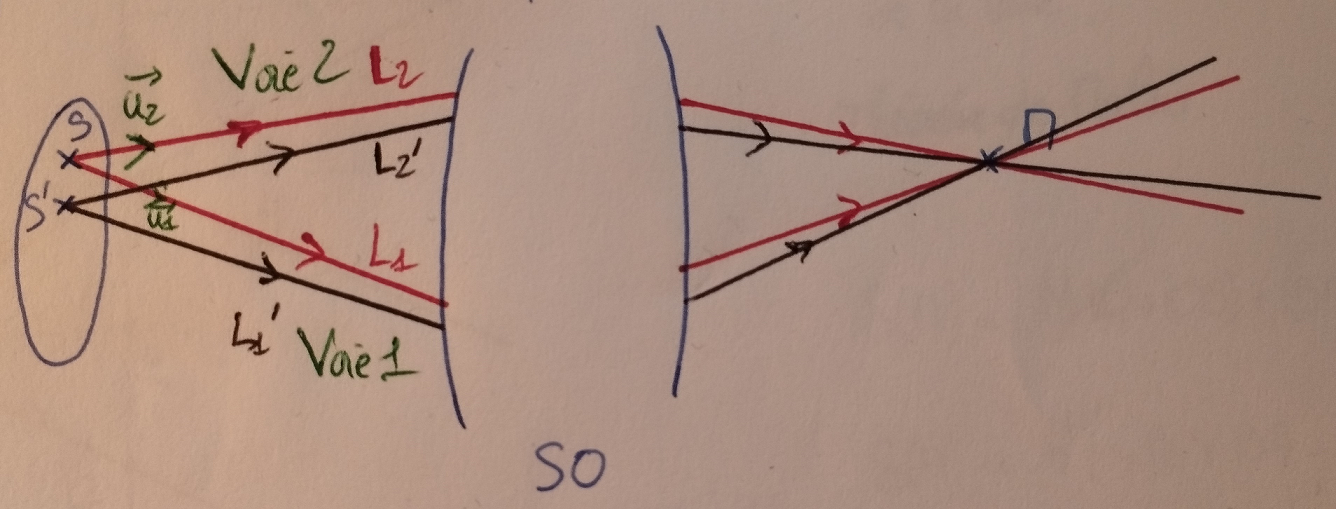
\includegraphics[scale=0.6]{LP_DivisionAmplitude/localisation.jpg}
  \caption{\label{fig:localisation}Système interférométrique (SO) éclairé par une source étendue. Les voies 1 et 2 constituent les voies de l'interféromètre. S et S' sont deux points sources.}
  \end{figure}
  
  \begin{figure}[!htbp]
  \centering
  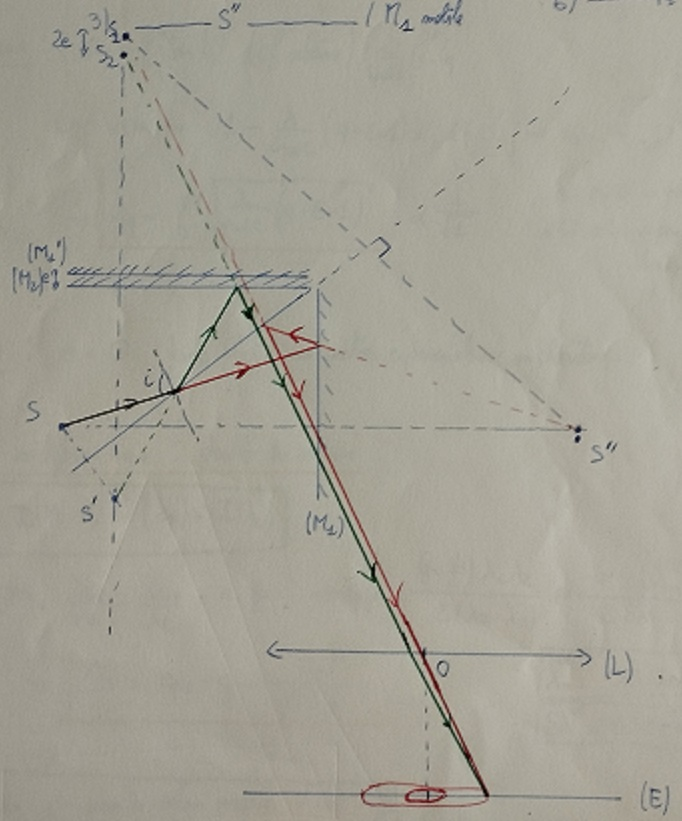
\includegraphics[scale=0.4]{LP_DivisionAmplitude/Michelson.jpg}
  \caption{\label{fig:Michelson}Schéma équivalent du Michelson. S$_1$ et S$_2$ sont les images de S à travers respectivement la voie 1 (Miroir M1) et la voie 2 (miroir M2) de l'interféromètre. Le miroir (M1') est l'image de (M1) à travers la séparatrice.}
  \end{figure}
  \clearpage
  
  

%%%%%%%%%%%%%%%%%%%%%%%%%%%%%%%%%%%%%%%%%%%%%%%%%%%%
%%%% Questions
\begin{reportBlock}{Questions posées par l’enseignant (avec réponses)}
  \begin{enumerate}
      \item Types d'interférence pour le casque anti-bruit ? \\ \textcolor{purple}{Il y a un micro qui permet d'enregistrer le bruit ambiant. Le signal est ensuite analysé puis un haut-parleur génère un signal de bruit avec une phase exactement opposée à celui qui vient d'être enregistré pour que les deux signaux interfèrent destructivement. Il s'agit donc d'une division du front d'onde.}
      
      \item Utilisation des intérférences à division d'amplitude ? \\
       \textcolor{purple}{Regarder la structure spatiale d'un l'échantillon, voir des défauts de planéité des miroirs, mesurer la différence d'indice de réfraction d'un gaz, mesurer une variation de température}. 
       
    \item Comment mesure-t-on l'indice de réfraction d'un gaz ? \\
       \textcolor{purple}{En configuration lame d'air, on peut regarder comment changent les franges rectlignes lorsque l'indice de refraction $n$ du milieu varie. Connaissant la taille du miroir, on peut remonter à $n$.}
       
      \item Quelle configuration pour la planéité des miroirs ? \\
       \textcolor{purple}{Configuration coin d'air.}
       
      \item En configuration coin d'air, où sont localisées les intérférences ? \\
       \textcolor{purple}{On verra des franges au niveau des miroirs.}
       
     \item Pourquoi au niveau des miroirs ? \\
       \textcolor{purple}{Il faut considérer deux points sources $S_1$ et $S_2$ proches et tracer les rayons issus de ces points et passant par un point $P$. Si $P$ est proches du coin d'air, la différence de marche $\delta_1$ entre les rayons issus de $S_1$ et celle entre les rayons issus de $S_2$ sont quasiment les mêmes (et égales à $2e(P)$): il n'y a donc pas brouillage. En revanche, si $P$ s'éloigne du coin d'air, $\delta_1$ devient très différent de $\delta_2$ et on a brouillage (cf. corrigé du TD d'optique sur les intéreférences). \\
       Par ailleurs, une construction géométrique permet de montrer que le lieu d'intersection des rayons réfléchis correspondant \textbf{à un même rayon incident} (condition de localisation vu en $1.1$, à savoir $\mathbf{u_2} = \mathbf{u_1}$) est approximativement le plan faisant l'angle $i$ (où $i$ est l'angle d'incidence) avec (M1'). En pratique, cet angle est si petit (quelques minutes d'arc) que ce plan d'intersection est presque confondu avec (M1') (Dunod Physique tout-en-un 2ème année, PC-PC* 2004).}
    
    \item Lorsque la source est ponctuelle, les interférences sont-elles localisées ? \\
       \textcolor{purple}{Non. Elles le sont lorsque la source est étendue.}
       
    \item Si on a des trous d'Young et une source déplacée de $b$ sur l'axe parallèle à l'axe des trous, comment seront les franges ? \\
       \textcolor{purple}{Il y aura une différence de chemin optique additionnelle avant les trous. Les nouvelles franges obtenues se décalent de $\frac{-bD}{d}$, avec $d$ la distance entre la source et les trous d'Young et $D$ la distance entre les trous et l'écran.}
    
    \item Peut-il y avoir brouillage si on considère deux sources ponctuelles incohérentes ?\\
    \textcolor{purple}{Oui si les deux systèmes de franges créés par les sources sont en anticoïncidence (les franges brillantes d'un système de franges se superposent aux franges sombres de l'autre système de franges).}
       
    \item Pour la lame d'air, pourquoi appelle-t-on les anneaux "anneaux d'égale inclinaison" ? \\
       \textcolor{purple}{Un ordre d'interférence donné correspond à une inclinaison, c'est-à-dire à un même angle d'incidence des rayons lumineux.}
       
    \item Pour la lame d'air, est-ce qu'on a le même signe de refléxion des deux côtés ? \\
       \textcolor{purple}{Non, $r_1 < 0$, $r_2 > 0$. Il y a un déphasage de $\pi$ en plus. Dans le Michelson, on oublie car c'est plus compliqué que ça, il y a des traitements en plus. Ce qui compte c'est que le contact optique est défini non pas par la longueur géométrique mais par la longueur optique.}
    
    \item A quoi sert la compensatrice ? On pourrait s'en passer pour le laser en réglant la longueur entre les deux bras de sorte à compenser la différence de marche correspondant à l'épaisseur de la séparatrice. \\
       \textcolor{purple}{Si la source est polychromatique, on ne peut pas trouver un pas du miroir qui compense la différence de marche pour toutes les longueurs d'onde car l'indice optique de la séparatrice dépend de la longueur d'onde, d'où la nécessité d'utiliser une compensatrice. Si une seule longueur d'onde, ce n'est pas nécessaire (mais ça n'existe pas dans la vraie vie).}
    
    \item Pourquoi tu utilises un verre anticalorique ? \\
    \textcolor{purple}{Pour ne pas diffuser de la chaleur provenant de la source sur l'interféromètre, cela modifierait $n$ qui dépend de la température (le Michelson est sensible à des variations d'indice de réfraction de l'ordre de $10^{-4}$.)}
       
    \item Le laser He-Ne : 10 MHz. Lorsqu'on a fait le calcul on a trouvé 400 MHz. Pourquoi cette différence ? \\
       \textcolor{purple}{En réalité, le spectre comporte plusieurs raies. L'enveloppe est à 400 MHz mais la largeur de chaque raie est beaucoup moins: 10 MHz semble raisonnable.}

       
    \item Que mesures-tu dans la tomographie ? \\
       \textcolor{purple}{Les interférences associées à une certaine épaisseur.}
      
  \end{enumerate}
\end{reportBlock}


%%%%%%%%%%%%%%%%%%%%%%%%%%%%%%%%%%%%%%%%%%%%%%%%%%%%
%%%% Commentaires
\begin{reportBlock}{Commentaires lors de la correction de la leçon}
\end{reportBlock}


%%%%%%%%%%%%%%%%%%%%%%%%%%%%%%%%%%%%%%%%%%%%%%%%%%%%
%%%% Correction

\begin{reportBlock}{Partie réservée au correcteur}
  \textbf{Avis général sur la leçon (plan, contenu, etc.) :}
  
  
  \textbf{Notions fondamentales à aborder, secondaires, délicates :}
  
  
  \textbf{Expériences possibles (en particulier pour l'agrégation docteur) :}
  
  
  \textbf{Bibliographie conseillée :}
\end{reportBlock}

\newpage
%%%%%%%%%%%%%%%%%%%%%%%%%%%%%%%%%%%%%%%%%%%%%%%%%%%%
%%%% En-tête leçon
\begin{headerBlock}
  \chapter{Diffraction de Fraunhofer.}
  \label{LP_DiffractionFraunhofer} 
\end{headerBlock}




%%%%%%%%%%%%%%%%%%%%%%%%%%%%%%%%%%%%%%%%%%%%%%%%%%%%
%%%% Références
\begin{center}
\begin{tabularx}{\textwidth}{| X | X | c | c |}
  \hline
  \rowcolor{gray!20}\multicolumn{4}{c}{Bibliographie de la leçon : } \\
  \hline 
  Titre & Auteurs & Editeur (année) & ISBN \\
  \hline
  Tout-en-un PC/PC* & M.-N. Sanz & Dunod (2022) & \\
  \hline
  Optique - Fondements et applications & J.P. Pérez & Dunod (2011) & \\
  \hline
  \url{https://www.lkb.upmc.fr/cqed/teaching/teachingsayrin/} & C. Sayrin & & \\
  \hline
  Optique Physique & R. Taillet & de boeck (2015) & \\
  \hline
  Optique Physique & D. Mauras & PUF (2001) & \\
  \hline
\end{tabularx}
\end{center}

%%%%%%%%%%%%%%%%%%%%%%%%%%%%%%%%%%%%%%%%%%%%%%%%%%%%
\begin{reportBlock}{Commentaires des années précédentes :}
    \begin{itemize}
        \item \textbf{2017 :} Les conditions de Fraunhofer et leurs conséquences doivent être présentées, ainsi que le lien entre les dimensions caractéristiques d’un objet diffractant et celles de sa figure de diffraction,
        \item \textbf{2014-2011 :} Les conditions de l’approximation de Fraunhofer doivent être clairement énoncées. Pour autant, elles ne constituent pas le coeur de la leçon.
    \end{itemize}
\end{reportBlock}
%%%%%%%%%%%%%%%%%%%%%%%%%%%%%%%%%%%%%%%%%%%%%%%%%%%%
%%%% Plan
\begin{reportBlock}{Plan détaillé}

  \textbf{Niveau choisi pour la leçon :} Licence 3
  \newline
  \textbf{Prérequis} : 
  \begin{itemize}
      \item optique géométrique,
      \item modèle scalaire des ondes lumineuses,
      \item transformées de Fourier,
      \item microscopie optique ?
  \end{itemize}
  \importantbox{Le message essentiel de la leçon est que la figure de diffraction de Fraunhofer se trouve dans le plan image de la source qui éclaire l’objet diffractant}
  \section*{Introduction}
  
  \section{Conditions de Fraunhofer de la diffraction}

  \subsection{Principe d'Huygens-Fresnel} 
  Voir Pérez p263. Enoncé, faire le dessins. Introduire le facteur d'obiquité et dire qu'il est constant si on considère des rayons proches de l'axe optique.\\
  La démo de Huygens-Fresnel est sur Wikipédia \url{https://fr.wikipedia.org/wiki/Th\%C3\%A9orie_de_Kirchhoff}.\\
  Donner l'amplitude scalaire de l'onde $s(M)$ (prendre les notations de C. Sayrin).

  \subsection{Amplitude d'une onde à travers un diaphragme plan}
  Cf TD Clément Sayrin Diffraction (1).\\

  \importantbox{On peut garder $\frac{e^{ikr}}{r}\sim\frac{e^{ikr}}{D}$ mais pour évaluer la phase $\mathbf{k}\cdot \mathbf{PM}$, il faut tenir compte des variations de PM=r à l’échelle de $\lambda$ et l’on garde donc les ordres plus élevés du développement.}

  \subsection{Conditions et approximations de Fraunhofer}
  On néglige le terme quadratique en $r^2$ dans la phase de l'onde. Enoncer les conditions pour avoir le terme de Fraunhofer nul voir Sextant p139 :
  \begin{itemize}
      \item onde plane ($d=0$) à l'infini ($D=0$), il suffit de placer une source lumineuse dans le plan focal objet d'une lentille convergente et observer la figure dans le plan focal image d'une autre lentille convergente,
      \item en pratique, condition pas très restrictive car : onde plane (source à l'infini) mais $kr^2<<2D\Leftrightarrow D>>\frac{r^2}{4\lambda}$. Application numérique : pour un laser de longueur d'onde $\lambda=648nm$, on trouve $D>>500m$ et si $r=1cm$, $D>>5m$ si $r=1mm$, $D>>5\mu m$ si $r=1\mu m$. Il est très facile d'être dans les conditions de Fraunhofer pour les petits objets diffractants ! Pour les objets plus grand, il faut faire l'image de la source lumineuse par une lentille,
      \item cas particulier de la source sur l'écran (d=-D) (à omettre, garder pour les questions ?)
  \end{itemize}
  On voit quand même que l'amplitude de l'onde résultante est la transformée de Fourier de la fonction $t(x,y)$ de l'objet diffractant. Il y a une relation de réciprocité entre les distances angulaires de la figure de diffraction et les distances dans le plan d'ouverture de l'objet diffractant.

  \textcolor{red}{Transition :} on va mettre en application ce qu'on vient de détailler en observant la figure de diffraction d'objets simples.
  \section{Exemples de systèmes diffractants}
  
  \subsection{Diffraction par une fente}
  Faire le calcul + la manip. Il faut juste prendre $t(x,y)=rect_x(-a/2,a/2)$.\\
  \textcolor{blue}{Manip qualitative : mesure d'une largeur de fente}. Voir Poly TP Montrouge Diffraction. On a besoin 
  \begin{itemize}
      \item barette CCD + logiciel MIGHTEX,
      \item laser + boys + lentille f=50mm,
      \item ordinateur avec Spectra Suite + câble connexion caméra,
      \item fentes sources de différentes taille + fente de taille variable,
  \end{itemize}
  

  \subsection{Diffraction par un trou d'Young}
  Le faire rapidement sur slide ou en estimant à l'aide de la formule précédente : un trou de rayon $a$ est contenu entre deux carrés de côté $\sqrt{2}a$ donc :
  \begin{equation}
      \frac{\lambda}{a} < \theta < \frac{\sqrt{2}\lambda}{a}\sim 1.4\frac{\lambda}{a}
  \end{equation}
  En prenant la moyenne : $\theta \sim (1.2\pm0.2)\frac{\lambda}{a}$. Le calcul se fait dans le Taillet p154.\\
  Conséquence voir Perez p276-277 : 
  \begin{itemize}
      \item parler du critère de Rayleigh donnant la résolution latérale maximale d'un microscope optique standard,
      \item \textcolor{red}{Attention, nécessite le théorème de Babinet} : tâches de diffraction circulaire autour de la Lune attribuées aux goutellettes d'eau/glace dans l'atmosphère. Calcul du diamètre des gouttes d'eau : $\theta=\frac{1.22\lambda}{D}$, si on prend $\theta\sim6\theta_{L}=0.5\degree$, on trouve en prenant $\lambda=600nm$ : $D=\frac{}{}$
  \end{itemize}
  Apodisation voir Mauras p258: pour observer les exoplanètes de faible intensité lumineuse proche des étoiles qui ont une très grande intensité lumineuse, on peut choisir de mettre un masque dont la fonction de transmission de la lentille décroît de l'unitéen son milieu à zéro à son bord : réduit l'intensité de des lobes secondaires de diffraction d'un objet très lumineux.
  
  \subsection{Ensemble de structure diffractante (peut sauter si besoin, ou en ouverture)}
  Si on prend pleins de trous d'Young et qu'on connait leur répartition spatiale, 

  \section{Applications de la diffraction}
  Au choix : expérience d'Abbe avec le filtrage spatiale, microscopie à contraste de phase,
  \section{}

  \section*{Conclusion}
  Ouverture sur la diffraction des rayons X. Conditions de Laue.

\end{reportBlock}
\newpage 
%%%%%%%%%%%%%%%%%%%%%%%%%%%%%%%%%%%%%%%%%%%%%%%%%%%%
%%%% En-tête leçon
\begin{headerBlock}
  \chapter{Diffraction sur des structures périodiques}
    \label{LP_DiffractionPeriodique}
\end{headerBlock}

%%%%%%%%%%%%%%%%%%%%%%%%%%%%%%%%%%%%%%%%%%%%%%%%%%%%
%%%% Références
\begin{center}
\begin{tabularx}{\textwidth}{| X | X | c | c |}
  \hline
  \rowcolor{gray!20}\multicolumn{4}{c}{Bibliographie de la leçon : } \\
  \hline 
  Titre & Auteurs & Editeur (année) & ISBN \\
  \hline
   Physique du solide & Ashcroft et Mermin & EDP Sciences &   \\
  \hline 
   Tout-en-un MP & M.-N. Sanz & Dunod (2009) &  \\
  \hline 
  Optique & J.-P. Pérez & Dunod & \\
  \hline 
  Optique Physique et électronique & D. Mauras & PUF (2011) & \\
  \hline
  \url{http://ressources.univ-lemans.fr/AccesLibre/UM/Pedago/physique/02/optiondu/reseauphase.html} & Simulation réseau & Université du Mans & \\
\end{tabularx}
\end{center}

\begin{reportBlock}{Commentaires des années précédentes :}
    \begin{itemize}
        \item \textbf{2017 :} Il faut traiter de diffraction par des structures périodiques et pas seulement d’interférences à N ondes,
        \item \textbf{2015 :} Il est important de bien mettre en évidence les différentes longueurs caractéristiques en jeu,
        \item \textbf{2014-2012 :} Cette leçon donne souvent l’occasion de présenter les travaux de Bragg ; malheureusement, les ordres de grandeur dans différents domaines ne sont pas toujours maîtrisés,
        \item \textbf{2010-2009 :} La notion de facteur de forme peut être introduite sur un exemple simple. L’influence du nombre d’éléments diffractants doit être discutée.
    \end{itemize}
\end{reportBlock}

%%%%%%%%%%%%%%%%%%%%%%%%%%%%%%%%%%%%%%%%%%%%%%%%%%%%
\begin{reportBlock}{Plan détaillé}
  \textbf{Niveau choisi pour la leçon :} Licence
  \newline
  \textbf{Prérequis : }
  \begin{itemize}
      \item Principe de retour inverse de la lumière, théorème de Malus
      \item Diffraction de Fraunhofer, diffraction par une fente rectangulaire
      \item notion de cohérence spatiale et temporelle
  \end{itemize} 

  
  \textbf{Déroulé détaillé de la leçon: }   \newline
La diffraction, en particulier dans les conditions de  Fraunhofer, permet de faire le lien entre les caractéristiques de l’objet diffractant et la figure de diffraction résultante. On va dans cette leçon s'intéresser aux propriétés d'objet diffractant possédant des structures périodiques et montrer en particulier deux choses : 1) si on connait les caractéristiques de l'objet diffractant, on peut connaitre les caractéristiques de la source, 2) on peut utiliser la figure de diffraction pour remonter à la structure interne de l'objet diffractant. On verra quelles limitations on obtient dans ces deux visions.\\

L'objet périodique par excellence est le réseau.

  \section{Diffraction par un réseau}
  Voir D. Mauras p194.
  \subsection{Définition}
  Il en existe de différents types (amplitude par transmission, phase par transmission, amplitude par réflexion (spectrographe) et phase par réflexion). On va s'intéresser pour l'instant aux réseaux d'amplitude par transmission. Faire un dessin en définissant le pas du réseau.

  \subsection{Formule fondamentale du réseau}
  On va considérer ici un montage de type Fraunhofer (source à l'infini, observation à l'infini) : faire le dessin (voir D. Mauras p195) en forçant le trait sur le réseau pour faire apparaitre l'angle $\theta_0$. Les ondes diffractées par les fentes donnent lieu à des interférences non localisées. On les observe à l'infini dans la direction $\theta$, réalité dans le plan focal de la lentille (L$_2$) au point M(x). Le principe de retour inverse (source fictive en M) et le théorème de Malus nous permet de montrer que \textcolor{red}{pour avoir interférences constructives} au point d'observation M :
  \begin{equation}
      \sin\left(\theta_p\right) - \sin\left(\theta_0\right) = \frac{p\lambda_0}{na}
  \end{equation}
  qui est la formule fondamentale des réseaux. Remarque : pour un réseau blazé (cf \url{http://olivier.sigwarth.free.fr/CoursTS2/Ch5/Chap5.pdf}), on remplace $\sin(\theta_p)$ par $\sin(\theta_p+\alpha)$. $p$ est l'ordre d'interférence :
  \begin{itemize}
      \item $p=0$ : la lumière se propage en ligne droite selon les lois de l'optique géométrique,
      \item l'ordre d'interférence est borné car $-1\leq sin(\theta_p)\leq 1 \rightarrow |p|\leq \frac{a}{\lambda}$ donc plus a est grand, plus on peut avoir des ordres d'interférences élevés. Plus la longueur d'onde est faible, plus il y a d'ordres d'interférences. Ex : pour un réseau à 500 traits/mm, si $\lambda=550$~nm, p=-3, -2, -1, 0, 1, 2 ,3 (7 ordres d'interférences).
  \end{itemize}
  Utilisation en lumière polychromatique : comme $\theta_p$ dépend de $\lambda$, le réseau est donc un disperseur de la lumière. D'autre part :
  \begin{align*}
      d\theta_p\cos(\theta_p) &= p\frac{d\lambda}{a} \\
      \frac{d\theta_p}{d\lambda} &= \frac{p\lambda}{a\sqrt{1-(sin(\theta_0)+p\frac{\lambda}{a})^2}}
  \end{align*}
  On commente :
  \begin{enumerate}
      \item Pour un ordre donné, la dispersion augmente avec la longueur d'onde contrairement au prisme,
      \item la dispersion augmente avec l'ordre d'interférence,
  \end{enumerate}
  On va voir visuellement tout ça à l'aide de l'expérience ci-après.
  
  \subsection{Mesure des raies spectrales de la lampe à vapeur de mercure}
  On va ici faire une application de l'utilisation des réseaux.\\
  Matériel :
  \begin{itemize}
      \item un réseau (prendre celui où on peut changer le pas du réseau ENSP 3637), choisir le 3000 traits/mm,
      \item lampe à vapeur de mercure + condenseur de 8cm,
      \item une lentille convergente de 15-20cm de focale + une autre de focale 10cm,
      \item une fente réglable,
      \item un écran blanc avec une feuille blanche et du scotch
      \item un miroir, une règle de 1m (ou un mètre).
  \end{itemize}
  \textcolor{blue}{Expérience quantitative :} On dispose d'une source à vapeur de mercure. On fait passer la lumière par une fente source de largeur réglable. On met une lentille de focale 15-20cm pour faire une image sur un écran éloigné. On intercale un réseau entre les deux. On oriente le réseau pour obtenir le minimum de déviation. On mesure l'angle $\tan{D_{p,min}}=\frac{d_{ecran}}{L_{ecran-reseau}}$. On en déduit $\lambda$ (avec incertitudes) la formule des réseaux à l'angle de déviation minimum.\\
  
  Mettre sur slide l'angle de déviation minimum :
  \begin{align*}
      D_p &= \theta_p - \theta_0 \\
      \sin{\theta_p} &= \sin(\theta_0) + p\frac{\lambda}{a} \\
      \frac{dD_p}{d\theta_0} &= \frac{\cos(\theta_0)}{\cos(\theta_p)}-1 =0 \rightarrow \cos(\theta_p)=\cos(\theta_0) \\
  \end{align*}
  Dériver $D_p$ une seconde fois par rapport à $\theta_0$ pour montrer que c'est un angle de déviation minimum. En prenant $\theta_{p,min}=-\theta_{0,min}$, le rayon émergeant est symétrique du rayon incident par rapport au plan du réseau et l'angle de déviation vaut :
  \begin{equation}
      2\sin\left(\frac{D_{p,min}}{2}\right) = p\frac{\lambda}{a}
  \end{equation}

  \textcolor{red}{Transition :} Ce qu'on a vu pour l'instant c'est qu'on peut mesurer le spectre d'émission d'une source polychromatique. Quelles sont ses limitations ? Il faut étudier plus en détail l'intensité résultante à travers une struture périodique la structure des pics d'interférences.

  \section{Facteur de structure et facteur de forme}
  
  \subsection{Intensité de la diffraction}

  \section{Application : diffraction des solides cristallins}
  Voir Kittel Chapitre 2.
  \subsection{Conditions de diffraction de Bragg}
  La condition des interférences contructives entre deux plans réticulaires séparés par la distance d s'écrit :
  \begin{equation}
      2d\sin{\theta} = n\lambda
  \end{equation}
  \textbf{Remarque :} pour qu'il y ait diffraction, on doit avoir $2d\sim 5\angstrom\leq\lambda$ ce qui montre qu'on ne peut pas utiliser la lumière pour résoudre la structure cristalline.


\section*{Conclusion}
Ouverture sur la diffraction des rayons X. Tâches de diffraction des papillons.
\end{reportBlock}




\newpage 
%%%%%%%%%%%%%%%%%%%%%%%%%%%%%%%%%%%%%%%%%%%%%%%%%%%%
%%%% En-tête leçon
\begin{headerBlock}
  \chapter{Absorbtion et émission de la lumière}
    \label{LP_Absorption}
\end{headerBlock}

%%%%%%%%%%%%%%%%%%%%%%%%%%%%%%%%%%%%%%%%%%%%%%%%%%%%
%%%% Références
\begin{center}
\begin{tabularx}{\textwidth}{| X | X | c | c |}
  \hline
  \rowcolor{gray!20}\multicolumn{4}{c}{Bibliographie de la leçon : } \\
  \hline 
  Titre & Auteurs & Editeur (année) & ISBN \\
  \hline
  Optique Physique & R. Taillet & de Boeck &   \\
  \hline 
  Physique Statistique & Landau et Lifshitz & Ellipses &  \\
  \hline 
   Poly laser & A. Maitre &  &  \\
\hline
 Sextant & & Hermann & \\
 \hline 
 Tout-en-un PC/PC* & M.-N. Sanz & Dunod & \\
 \hline 
 Physique en PC/PC* & Pascal Olive & Ellipses & \\
 \hline
\end{tabularx}
\end{center}

%%%%%%%%%%%%%%%%%%%%%%%%%%%%%%%%%%%%%%%%%%%%%%%%%%%%
\begin{reportBlock}{Plan détaillé}
  \textbf{Niveau choisi pour la leçon :} Licence
  \newline
  \textbf{Prérequis : }Milieu LHI, distribution de Boltzmann
  \newline
  
  \textbf{Déroulé détaillé de la leçon: }   \newline
On verra deux modèles qui permettront d'expliquer le phénomène d'émission et absorption de la lumière dans les milieux.
  \section{Modèle de Lorentz}
  
  \subsection{Electron élastiquement lié}
  Modèle classique : électron gravite autour d'un proton et voit le champ électrique de la lumière $\mathbf{E}$. Un bilan des forces conduit à :
  \begin{itemize}
      \item Force de Lorentz : $-e\mathbf{E}$
      \item Force de rappel : $-K\mathbf{r}$
      \item phénomène dissipatif : $-\frac{m_e}{\tau}\mathbf{E}$
  \end{itemize}
Le PFD donne :
\begin{equation}
    \frac{d^2\mathbf{r}}{dt^2} + \frac{\omega_0}{Q}\frac{d\mathbf{r}}{dt} + \omega^2\mathbf{r} = \frac{-e\mathbf{E}}{m_e}
\end{equation}
avec $Q=\omega_0\tau$ et $\omega_0=\sqrt{\frac{K}{m_e}}$.\\

Soit le moment dipolaire $\mathbf{p}=-e\mathbf{r}$ et le vecteur polarisation $\mathbf{P}=N\mathbf{p}=\epsilon_0\chi_e\mathbf{E}$ dans un milieu LHI. On choisit un champ $\mathbf{E}=\mathbf{E_0}\exp{j(\omega t - \mathbf{k}\cdot\mathbf{r})}$ et on en déduit : 
\begin{equation}
    \chi_e = \frac{\chi_0}{1 + jQ\frac{\omega}{\omega_0}-(\frac{\omega}{\omega_0})^2}
\end{equation}
avec $\chi_0=\frac{Ne^2}{n_e\epsilon_0\omega_0^2}$\\

Problème : ce modèle ne prend pas du tout en compte l'émission de la lumière. Il faut alors introduire le modèle d'Einstein sur l'émission.

\section{Modèle d'Einstein}
\subsection{Equation d'Einstein}
Soit un système à deux niveaux d'énergie $E_a$ et $E_b$ associée aux états propres $\ket{a}$ et $\ket{b}$. On note $N_a$ et $N_b$ la population de ces niveaux telles que $N_a+N_b=N$. La proba d'occupation est $n_i=\frac{N_i}{N}$.\\
La lumière que reçoit ce système est caractérisé par une densité spectrale $u(\nu)=\frac{dU}{d\nu}$ avec $U=\frac{\epsilon_0E^2}{2}+\frac{B^2}{2\mu_0}$.\\


A l'équilibre : $\frac{dn_a}{dt}=-\frac{dn_b}{dt}$ et donc : 
\begin{equation}
    \frac{dn_a}{dt} = -An_b + B_{21}u(\nu_0)
\end{equation}
\subsection{Coefficients d'Einstein}

En posant $h\nu_0 = E_b - E_a$, on a $\frac{n_a}{n_b}=\exp{-\frac{E_a+E_b}{k_BT}} = \exp{\frac{h\nu_0}{b_BT}}$. On en déduit que $B_{12} = B_{21} = B$ et $\frac{A}{B}=\frac{8\pi h\nu_0^3}{c^3}$. L'équation d'Einstein devient : 
\begin{equation}
    \frac{dn_b}{dt} = -\frac{dn_a}{dt} = -An_a + Bu(\nu_0)(n_a-n_b)
\end{equation}

\subsection{Processus de transfert d'énergie}
La puissance transférée de l'atome vers le champ $P_{at\rightarrow ch}=-h\nu_0\frac{dn_b}{dt} = h\nu_0B(n_b-n_a)u(\nu_0)$. On distingue alors deux régimes : 
\begin{itemize}
    \item Si $n_a>n_b$, $P_{at\rightarrow ch}<0$ $\longrightarrow$ Absorbtion
    \item Si $n_a<n_b$, $P_{at\rightarrow ch}>0$ $\longrightarrow$ Inversion de population
\end{itemize}

Initialement $n_a=1$,$n_b=0$ : 
\begin{itemize}
    \item $n_a(\infty) = \frac{A + Bu(\nu_0)}{A + 2Bu(\nu_0)}$
    \item $n_b(\infty) = \frac{Bu(\nu_0)}{A + 2Bu(\nu_0)}$
\end{itemize}
\end{reportBlock}


\begin{reportBlock}{Questions posées par l’enseignant (avec réponses)}
  \textbf{C : Que peut-on dire sur le mouvement dans le modèle élastiquement lié ?}  \textcolor{purple}{Il y a une force centrale (force électrostatique) donc on a des mouvements circulaires.} Uniquement circulaires ? \textcolor{purple}{Non, il peut y avoir des trajectoires elliptiques qui sont des solutions pour un état lié (comme le système \{planète-Soleil\} pour la gravité).} \newline
  \textbf{C : Pas d'interaction répulsive ?}  \textcolor{purple}{La force de rappel élastique est répulsive si l'allongement est plus faible que la longueur à vide.}\\
  \textbf{C : Pourquoi il y a un phénomène dissipatif ?}  \textcolor{purple}{Je ne sais plus. Un électron accéléré perd forcément de l'énergie par rayonnement (dipolaire par exemple), sinon il peut avoir une vitesse infinie.}\\
  \textbf{C : Le champ $\mathbf{E}$ n'est pas uniforme si ?}  \textcolor{purple}{La longueur d'onde du champ est très grande devant la taille de l'atome donc on peut le considérer uniforme.} Y-a-t'il quand même un effet ? Le proton est-il fixe ? \textcolor{purple}{Oui le proton bouge, il faudrait se placer dans le référentiel du centre de masse. Mais comme $m_{proton}>>m_{e^-}$, ça ne change pas vraiment la position du problème.}\\
  \textbf{C : C'est quoi le lien entre le modèle de Lorentz et le titre de la leçon ?} \textcolor{purple}{Je voulais arriver jusqu'à la définition des indices optiques.} Qu'est-ce que ce modèle prédit ? Où va l'énergie ? \textcolor{purple}{Ce modèle prédit l'évolution de la polarisabilité électronique en fonction de la fréquence de l'onde incidente. Pour certaines fréquences, le dipôle absorber un photon et s'orienter et créer une polarisation d'origine  électronique. Voir le BFR Tome 4, Chapitre 4. L'énergie se transfert vers les phonons, dans le rayonnement dipolaire. C'est un phénomène de diffusion. Le transfert d'énergie se fait par l'intermédiaire de la partie imagnaire de la susceptibilité. En revanche ce modèle ne prédit pas d'amplification (énergie amenée par les atomes au champ électrique, en gros on ne peut pas avoir un photon à l'entrée = deux photons à la sortie).}\\
   \textbf{C : Revenons à l'interprétation des coefficients d'Einstein, les explications paraissaient un peu triviales} \textcolor{purple}{A : désexcitation spontanée car niveau b instable, B : désexcitation stimulée par le champ électrique. } Il y a un temps de vie des électrons sur les niveaux ? \textcolor{purple}{D'après le principe d'incertitude de Heisenberg $\Delta E\Delta t>\hbar/2$. Autrement dit, les électrons ont une durée de vie $\Delta t$ finie sur les niveaux d'énergie de largeur $\Delta E$.} C'est quoi le $\Delta E$ ? \textcolor{purple}{La largeur d'une bande d'énergie d'un niveau électronique.} Du coup c'est quoi la différence entre A et B ? \textcolor{purple}{A traduit le taux de probabilité liée à la désexcitation spontanée de l'atome (en $s^{-1}$), B est le taux de probabilité de transition $\ket{A}\rightarrow \ket{B}$ lié à l'absorption du rayonnement égal au taux d'émission stimulée $\ket{B}\rightarrow \ket{A}$.}\\
   \textbf{C : Pourquoi $u$ n'apparait pas dans l'émission spontanée ?} \textcolor{purple}{Ce terme n'est pas lié au rayonnement thermique mais au fait que les électrons ont une durée de vie finie sur le niveau d'énergie $\ket{b}$ du fait du principe d'incertitude d'Heisenberg.}
  
\end{reportBlock}



\newpage
%%%%%%%%%%%%%%%%%%%%%%%%%%%%%%%%%%%%%%%%%%%%%%%%%%%%
%%%% En-tête leçon
\begin{headerBlock}
  \chapter{Propriétés macroscopiques des corps ferromagnétiques}
  \label{LP_Ferromagnetisme} 
\end{headerBlock}




%%%%%%%%%%%%%%%%%%%%%%%%%%%%%%%%%%%%%%%%%%%%%%%%%%%%
%%%% Références
\begin{center}
\begin{tabularx}{\textwidth}{| X | X | c | c |}
  \hline
  \rowcolor{gray!20}\multicolumn{4}{c}{Bibliographie de la leçon : } \\
  \hline 
  Titre & Auteurs & Editeur (année) & ISBN \\
  \hline
  Électromagnétisme. Tome 4 - Milieux diélectriques et milieux aimantés & M. Bertin, J.P. Faroux et J. Renault  & Dunod (1984) &    \\
  \hline 
  Electromagnétisme - Fondements et applictions & J-Ph. Pérez & Dunod 4ème édition (2019) &    \\
  \hline 
  Physique Spé. PSI*, PSI & S. Olivier, C. More, H. Gié & Tec \& Doc (2000) &    \\
  \hline 
  Physique de l'état solide & C. Kittel & Dunod 7ème édition (1998) &    \\
  \hline
\end{tabularx}
\end{center}

%%%%%%%%%%%%%%%%%%%%%%%%%%%%%%%%%%%%%%%%%%%%%%%%%%%%
\begin{reportBlock}{Commentaires des années précédentes :}
    \begin{itemize}
        \item \textbf{2017 :} L’introduction des milieux linéaires en début de leçon n’est pas judicieuse,
        \item \textbf{2016 :} Un bilan de puissance soigné est attendu,
        \item \textbf{2010-2009 : }L’intérêt du champ H doit être clairement dégagé. L’obtention expérimentale du cycle d’hystérésis doit être analysée.
    \end{itemize}
\end{reportBlock}
%%%%%%%%%%%%%%%%%%%%%%%%%%%%%%%%%%%%%%%%%%%%%%%%%%%%
%%%% Plan
\begin{reportBlock}{Plan détaillé}

  \textbf{Niveau choisi pour la leçon :} Licence 3
  \newline
  \textbf{Prérequis} : \begin{itemize}
      \item Electrocinétique
      \item Induction
      \item Notions sur la paramagnétisme et le diamagnétisme
      \item Milieu LHI
  \end{itemize}

  \textbf{Déroulé détaillé de la leçon: }  
  
  \section*{Introduction}

Introduction sur les matériaux ferromagnétiques en prenant l'exemple de la magnétite (Fe$_2$O$_3$).
Définition : corps qui, sous l'action d'un champ EM extérieur, s'aimante très fortement.

\section{Aimantation d'un corps ferromagnétique (1min15)}

\subsection{Magnétostatique dans un milieu aimanté}

Dans la matière, il y a des électrons et des atomes qui portent des moments magnétiques. 

Définition de l'aimantation : $\mathbf M = \frac{\ud \mathbf m}{\ud t}$ (en A.m$^{-1}$).

Vecteur excitation magnétique : $\mathbf H = \frac{\mathbf B}{\mu_0} - \mathbf M$. 

Equation de Maxwell-Ampère : $\nabla \times \mathbf H j_{\text{libre}}$.
Equation de Maxwell-flux : $\nabla \cdot \mathbf B = 0$.

Pour un LHI : $\mathbf M = \chi_m \mathbf H$, avec $\chi_m$ la susceptibilité magnétiques.

Pour les milieux paramagnétiques et diamagnétiques, $\mid\chi_m \mid << 1$. Alors que pour les ferromagnétiques : 
\begin{itemize}
    \item $\chi_m(\mathbf H)$ : relation non linéaire entre $\mathbf M$ et $\mathbf H$.
    \item $\mid\chi_m \mid >> 1$
\end{itemize}

\subsection{Courbe de première aimantation (7min10)}

Courbe $M(H)$ pour un matériau ferrmoagnétique initialement non aimanté : (1) courbe linéaire pour les petits $H$ puis (2) fortement croissante puis (3) sature progressivement jusqu'à $M_{sat}$.

$\mu_0 M_{sat}$ est le champ magnétique maximal d'un ferromagnétique à $T$ donnée et dépend du matériau. $M_{sat}(Fe) = 2.1 T$


\subsection{Interprétation microscopique (9min12)}
Slide : Domaines de Weiss. Déplacement des domaines réversible à faible $B$, mais irreversible pour $B$ plus élevé du fait de la présence d'impuretés dans le matériau.\\

Une propriété des ferromagnétiques est la canalisation des lignes de champs magnétiques. Slide: illustrations pour différentes géométries. Pour un ferromagnétique torique, les lignes de champ sont complètement canalisées.

\section{Cycle d'hystérésis (14min)}

Présentation de l'expérience. Transformateur: un primaire et un secondaire. \textbf{C'est l'expérience "Étude du cycle d'hystérésis du fer d'un transformateur" du TP Conversion de puissance électrique, version 2023}.

\subsection{Etude du noyau de fer d'un transformateur(15min)}

Schéma électrique du montage (cf. TP Conversion de puissance électrique)

Théorème d'Ampère : $L H = n_1 i_1 + n_2 i_2$
$L$ : longueur totale du tore (fer doux), $n_i$ nombre de spires de la bobine $i$. $H = \frac{n_1 i_1 + n_2 i_2}{L}$ donne (avec $i_2$ négligeable devant $i_1$ car la résistance imposée dans le secondaire ($\sim 10$~k$\Omega$) associée est bien plus élevée que celle du primaire ($\sim 30$~$\Omega$)) $i_1 = \frac{L}{n_1} H$. Ainsi, si on mesure la tension aux bornes de la résistance du circuit primaire : 

$V_x = R i_1 = \frac{R L}{n_1} H$ avec ici $\frac{R L}{n_1} = 62.4 V/(Am^{-1})$ qu'on place sur la voie 1 de l'oscillo.

Dans le circuit secondaire, on a (Loi de Faraday) : $e = -\frac{\ud \phi}{\ud t} = -n_2 S \frac{\ud B}{\ud t} = R' i_2 + \int \frac{i_2}{C}$ (cf. TP). $R'$ et $C$ sont choisies de telle sorte que $\int \frac{i_2}{C}$ soit négligeable devant $R' i_2$. Il vient :

$i_2 = \frac{S}{R'} \frac{\ud B}{\ud t}$.

Conséquences, aux bornes du condensateur: $U_c = \int \frac{n_2 S}{c R'} \frac{\ud B}{\ud t} \ud t$. Finalement :

$V_y = U_c = \frac{n2 S}{R' C} B$ qu'on place sur la voie 2 de l'oscillo.

\subsection*{Début de l'expérience (24min45)}

\begin{itemize}
    \item Visualisation du cycle d'hystérésis avec le mode XY.
    \item Tracé du cycle $B(H)$ au tableau et définition du champ coercitif $H_c$ (pour $B=0$) et du champ rémanent $B_r$ (pour $H=0$).
    \item Mesure expérimentale de $B_r$. Valeurs : $V_y = 2.70 \pm 0.02$~V donne $B_r = 0.532 \pm 0.004 T$. 
    \item Mesure expérimentale de $H_c$. Valeurs : $V_x = 2.10 \pm 0.01$~V donne $H_c = 313 \pm 1$~A/m. Valeur caractéristique des ferro doux. Plus cette valeur est faible, plus l'excitation à devoir appliquer pour désaimanter le matériau sera faible: ce type de matériau se désaimante facilement.  
\end{itemize}

On distingue deux types de ferro (slide tableau comparatif). Ferro doux (Transformateurs, inductance à haute fréquence) et ferro durs (application générateur électrique, RMN, etc.).

\subsection{Bilan de puissance (35min38)}

Loi des mailles : $U i_1 + e i_1 - R i_1 = 0$. Premier terme: ; dernier terme : puissance dissipée par effet Joule. $e i_1 = - \frac{\ud \phi}{\ud t} i_1$. $\delta W = - \ud \phi i_1 = - \frac{SHL}{n_1} = \ud B$. $P = \frac{1}{T} SL \oint H _ud B$. ¨

\section*{Conclusion (39min50)}

Application : disques durs.
Fin : 40min35.

\end{reportBlock}


%%%%%%%%%%%%%%%%%%%%%%%%%%%%%%%%%%%%%%%%%%%%%%%%%%%%
%%%% Questions
\begin{reportBlock}{Questions posées par l’enseignant (avec réponses)}
  \textbf{Q: Si je lis votre relation, si j'augmente le nombre de spires, je vais diminuer la perte par hystérésis ?} \textcolor{purple}{Non, il y a une erreur dans ma formule, elle ne dépend pas du nombre de spires.} \newline
  
  \textbf{Q: Si je regarde le cycle d'hystérésis, le champ $B$ sature ?} \textcolor{purple}{Non, il continue à croître linéairement.} \newline
  
   \textbf{Q: Pourquoi on utilise des ferro doux pour l'inductance à haute fréquence.?} \textcolor{purple}{Ce qui compte dans une inductance c'est la variation du flux. Mais dans le ferro dur, quand c'est saturé, certes le champ est fort, mais il n'est plus sensible au champ extérieur. Un ferro doux, en première approximation, c'est linéaire et la pente est la susceptibilité. Mais pour le ferro dur, la pente est nulle.} \newline
  
  \textbf{Q: Pourquoi à haute fréquence ?} \textcolor{purple}{Pour minimiser les pertes par courants de Foucault.} \newline
  
   \textbf{Q: Quels matériaux qui minimisent ces pertes à hautes fréquence?} \textcolor{purple}{Utiliser des isolants (ferrites), on va limiter ainsi des pertes par courants de Foucault.} \newline
  
  \textbf{Q: Est-ce que la canalisation des champ est générique à tous les ferro ?} \textcolor{purple}{Ce n'est pas le cas pour les ferros durs, que pour les ferros doux. Toutes les applications qui utilisent $\chi$ ou $\mu_r$ très grand c'est les ferro doux, car il n'y a plus de pente pour les ferro durs.} \newline
  
   \textbf{Q: Dans quel état sont les ferromagnétiques ?} \textcolor{purple}{Solides cristallin. L'état ferro provient d'interaction au niveau des atomes qui n'existent pas à l'état fluide.} \newline
  
  \textbf{Q: L'aimantation à saturation et le champ coercitif dépendent des matériaux ?} \textcolor{purple}{Varie de quelques magnétons de Bohr mais reste du même ordre de grandeur alors que $H_c$ varie beaucoup : un ferro doux a un champ coercitif faible (10$^{-3}$~T), un ferro dur très grand (0.1~T) matériau à un autre.} \newline
  
   \textbf{Q: Sur l'histoire du transformateur, vous avez appliqué le théorème d'Ampère. C'est évident que $\oint H.\ud l = H L$ ? } \textcolor{purple}{Il faut utiliser les relations de passage des champs B et H pour démontrer la canalisation des lignes de champs dans le ferro en l'absence de courants surfaciques à l'interface fer$\rightarrow$air. Ensuite, les symétries et invariances du tore donnent $\mathbf{H}=H(r)\mathbf{e_{\theta}}$ et le théorème d'Ampère le long d'une ligne de champ permet d'avoir la formule donnée si on considère que la section du tore est faible devant la distance à l'axe.%Vous n'avez pas utilisé $\nabla \cdot B = 0$, il faut l'utiliser
   .} \newline
  
  \textbf{Q: Dans un éléctroaimant ?} \textcolor{purple}{Il n'y a pas conservation de la norme de $H$. Pour relier $H$ dans l'entre-fer et dans le milieu, il faut utiliser la conservation du flux.} \newline
  
   \textbf{Q: Pourquoi le système forme les domaines de Weiss ?} \textcolor{purple}{Au niveau microscopique, il y a une compétition entre l'énergie qu'il va falloir fournir pour créer ces interfaces et le coût en énergie pour créer un champ via l'alignement des moments magnétiques.} \newline
  
  \textbf{Q: La taille des domaines ?} \textcolor{purple}{De l'ordre du micromètre.} \newline
  
   \textbf{Q: Est-ce qu'il y a des directions priviligiées au départ dans champ extérieur? Est-ce que je peux avoir une courbe d'hystérésis qui dépend du champ $B$?} \textcolor{purple}{Oui, il y a un axe de facile aimantation. Les champs coercitifs vont être plus forts dans l'axe de facile aimantation. Cela va exister dans des monocristaux. Les axes de facile et difficile aimantation sont définis par rapport à l'orientation cristalline du matériau et des interactions entre les moments magnétiques dans le matériau. Il n'y a pas de raison pour que l'orientation du domaine soit dans la direction du champ appliqué.} \newline
  
  \textbf{Q:  Quels sont les conditions qui vous permettent de lire directement $B$?} \textcolor{purple}{$e = U_{R'} + U_c = R' i_2 + \frac{1}{jC\omega} i_2 = R'(1+\frac{1}{jRC\omega}) i_2$. On veut alors $R'C >> \frac{1}{\omega}$ avec $\omega=2\pi f$ et $f=50$~Hz (fréquence du secteur).} \newline
  
  \textbf{Q: Les applications des ferros durs?} \textcolor{purple}{Tous les aimants permanents. } 
  
 
  
  \end{reportBlock}
  
%%%%%%%%%%%%%%%%%%%%%%%%%%%%%%%%%%%%%%%%%%%%%%%%%%%%
%%%% Commentaires
\begin{reportBlock}{Commentaires lors de la correction de la leçon}

Agréable à suivre. Le rythme était un peu lent. Parfois vous vous répétez un peu, c'est très bien pour un vrai cours mais pas nécéssaire pour une leçon d'agrégation, ce qui permet de gagner un peu de temps pour la partie ferro dur/ferro doux qui est un point central, et aussi pour l'histoire du $\nabla \cdot B$. Ne pas faire la démonstration pour la canalisation est un choix, vous auriez pu le faire sur transparent pour gagner du temps. Votre exploitation de la manipulation est remarquable. Il faut donner les chiffres des ordres de grandeurs. 

\end{reportBlock}



%%%%%%%%%%%%%%%%%%%%%%%%%%%%%%%%%%%%%%%%%%%%%%%%%%%%
%%%% Correction
\begin{reportBlock}{Partie réservée au correcteur}
  \textbf{Avis général sur la leçon (plan, contenu, etc.) :}
  
  
  \textbf{Notions fondamentales à aborder, secondaires, délicates :}
  
  
  \textbf{Expériences possibles (en particulier pour l'agrégation docteur) :}
  
  
  \textbf{Bibliographie conseillée :}
\end{reportBlock}

\newpage
%%%%%%%%%%%%%%%%%%%%%%%%%%%%%%%%%%%%%%%%%%%%%%%%%%%%
%%%% En-tête leçon
\begin{headerBlock}
  \chapter{Mécanismes de la conduction électrique dans les solides}
    \label{LP_Conduction}
\end{headerBlock}

%%%%%%%%%%%%%%%%%%%%%%%%%%%%%%%%%%%%%%%%%%%%%%%%%%%%
%%%% Références
\begin{center}
\begin{tabularx}{\textwidth}{| X | X | c | c |}
  \hline
  \rowcolor{gray!20}\multicolumn{4}{c}{Bibliographie de la leçon : } \\
  \hline 
  Titre & Auteurs & Editeur (année) & ISBN \\
  \hline
Physique des Solides (Chap 1 à 3)  & N. Ashcroft et D.Mermin   &  EDP Sciences (2002) & 2-86883-577-5  \\
  \hline 
     Slides de cours & Gwendal Fève &  &  Site Montrouge \\
  \hline 
  Physique des Solides & C. Kittel &  Dunod &  \\
\hline
Site ferrarithierri pour télécharger BUP 550 & A. Guinier, E. Guyon, J Matricon, C. Taupin & BUP & \\
\hline 
\end{tabularx}
\end{center}

%%%%%%%%%%%%%%%%%%%%%%%%%%%%%%%%%%%%%%%%%%%%%%%%%%%%
\begin{reportBlock}{Commentaires des années précédentes :}
    \begin{itemize}
        \item \textbf{2017 :} Cette leçon ne concerne pas que la conduction dans les métaux,
        \item \textbf{2014 :} Dans la présentation du modèle de Drude, les candidats doivent être attentifs à discuter des hypothèses du modèle, en particulier celle des électrons indépendants. Le jury se permet par ailleurs de rappeler aux candidats que les solides ne sont pas tous métalliques.
    \end{itemize}
\end{reportBlock}
%%%%%%%%%%%%%%%%%%%%%%%%%%%%%%%%%%%%%%%%%%%%%%%%%%%%

%%%%%%%%%%%%%%%%%%%%%%%%%%%%%%%%%%%%%%%%%%%%%%%%%%%%

\begin{reportBlock}{Plan détaillé}

  \textbf{Niveau choisi pour la leçon :} 
  \newline
  \textbf{Prérequis} : \begin{itemize}
  \item loi d'Ohm, mécanique newtonienne,
      \item statistique de Maxwell-Boltzmann, modèle du gaz parfait,
      \item statistique de Fermi-Dirac
      \item 
  \end{itemize}
  
\section*{Introduction}
On connaît et on utilise trivialement l’électricité, ça fait partie de la culture générale scientifique de savoir qu’il existe des matériaux conducteurs et des matériaux isolants (c'est même quelque chose qu'on voit au collège avec des expériences permettant d'allumer une ampoule avec du caoutchouc, du bois, du cuivre, ...). On va voir dans cette leçon que cette notion naturelle n'est en réalité explicable que par la mécanique quantique et que les modèles classiques échouent à rendre compte expérimentalement ce qui se passe.

\section{Approche microscopique classique}
\subsection{Modèle de Drude (1902) 10min max}
%Définition résistivité : $\rho=\frac{RS}{L}$.\\
Contexte historique : découverte de l'électron par Thomson (1899), avant expérience de Rutherford.\\
Cristal métallique : [grosses sphères chargés + avec des électrons de c\oe ur] = ions métalliques  + électrons de valence pour assurer électroneutralité.\\
Remarque : $n_{gaz}=10^{25}$m$^{-3}$ tandis que $n_{e^{-}}=10^{29}$m$^{-3}$, cf p4 Ashcroft.\\
Hypothèses :\begin{itemize}
    \item pas d'interaction entre les électrons et les ions, et entre les électrons et les électrons : \textcolor{red}{"électrons libres"},
    \item \textcolor{red}{collisions et changement de vitesse instanées} entre les électrons de c\oe ur et les électrons de valence,
    \item électrons de valence (conduction) se déplacent en ligne droite jusqu'à collision avec proba $1/\tau$. $\tau$ est \textcolor{red}{le temps de collision} ou libre parcourt moyen, temps moyen de propagation entre deux chocs,
    \item \textcolor{red}{chaos moléculaire}, la distribution des vitesses suit une loi de Maxwell-Boltzmann comme le gaz classique, la direction des électrons est aléatoire. L'équilibre thermodynamique local des électrons avec leur entourage par le biais des collisions (seul mécanisme restant) : 
\end{itemize}

Ce modèle décrit relativement bien la conductivité dans un métal.
Déduire équation du mouvement + 
\subsection{Mise en défaut pratique du modèle de Drude}
Bien fait dans le BUP.\\
Voici ce que Drude prévoit en supposant que la vitesse des électrons obéit à la statistique de Boltzmann :
\begin{itemize}
    \item dans un modèle de gaz parfait, la vitesse moyenne des électrons est : $v^*=\sqrt{\frac{3k_BT}{m_e}}=\frac{l}{\tau}$ (utiliser le théorème d'équipartition.
    \item comme $\tau=\frac{\sigma m_e}{N_ee^2}$ avec le modèle de Drude, on obtient $\sigma\propto \frac{1}{\sqrt{T}}$
\end{itemize}

\textcolor{blue}{Manip quantitative : mesure 4 points d'un morceau de cuivre à différentes températures. Montrer (si possible) que la résistivité est linéaire en température.}\\
\begin{itemize}
    \item en utilisant $1/2mv^2=3/2k_BT$, on trouve $v=10^5$m/s alors que $v_{F}=10^6$m/s et indépendante de T,
    \item quid des matériaux isolants ? semi-conducteurs ?
    \item effet Hall classique dans l'aluminium (p18 Ashcroft) montre que n dépend fortement de B appliqué, ce qui est inenvisagable dans le modèle de Drude + constante de Hall parfois positive
\end{itemize}

Conclusion : il faut passer à un autre modèle plus poussé : un modèle quantique.

\section{Modèle quantique des électrons libres}
Electrons obéissent à la statistique de Fermi-Dirac et non à la statistique de Maxwell-Boltzmann.
\subsection{Modèle des électrons libres}
Cf Kittel chap 8 ou Ashcroft chap 2 et 13. Modèle de Sommerfeld. Faire les calculs Justifier qu'on peut se placer à T=0K.

\section{Théorie des bandes}

\subsection{Electrons dans un potentiel périodique}
Modèle : électrons en intéraction avec le potentiel périodique du réseau cristallins.\\
Cf Kittel (chap 7) + TD 1 Physique des Solides : mettre en prérequis pour les calculs.

\subsection{Bandes d'énergie}
Slide : schéma bande avec isolant+ tableau périodique 

\subsection{Remplissage des bandes}

Distinguer métaux, semi-conducteurs et isolant. Prévoir lesquels seront métalliques avec le demi-remplissage, lesquels seront isolants. Montrer que ça ne marche pas toujours.
\subsection{Conductivité dans un semi-conducteur}
Densité d'état varie en $\exp(-\Delta/k_BT)$ donc $\sigma$ aussi.\\

\textcolor{blue}{Mesure de la conductivité dans un semi-conducteur dopé pour déterminer le gap.}, cf TP semiconducteurs. Durée 30min environ, $\Delta_{exp}=0.6$eV alors que $\Delta_{th}=0.7$eV. Interprétation : matériel vieux, gap a pu changer. Matériau pas pur.\\
\section{Conclusion}
Ouverture sur l'ingénierie des semi-conducteurs : micro-électronique, jonctions pn, transistors. Prix Nobel 2014 pour l'invention de la diode bleue (en 1992).\\
Ouverture sur la supraconductivité (slide supra mercure).\\
Ouverture possible sur la conduction thermique, loi de Wiedemann-Franz.

\end{reportBlock}
\newpage
%%%%%%%%%%%%%%%%%%%%%%%%%%%%%%%%%%%%%%%%%%%%%%%%%%%%
%%%% En-tête leçon
\begin{headerBlock}
  \chapter{Phénomènes de résonance dans différents domaines de la physique}
  \label{LP_resonance} 
\end{headerBlock}

%%%%%%%%%%%%%%%%%%%%%%%%%%%%%%%%%%%%%%%%%%%%%%%%%%%%
%%%% Références
\begin{center}
\begin{tabularx}{\textwidth}{| X | X | c | c |}
  \hline
  \rowcolor{gray!20}\multicolumn{4}{c}{Bibliographie de la leçon : } \\
  \hline 
  Titre & Auteurs & Editeur (année) & ISBN \\
  \hline
  & & & \\
  \hline 
  & & &    \\
  \hline 
  & & &    \\
  \hline 
\end{tabularx}
\end{center}

%%%%%%%%%%%%%%%%%%%%%%%%%%%%%%%%%%%%%%%%%%%%%%%%%%%%
\begin{reportBlock}{Commentaires des années précédentes :}
    \begin{itemize}
        \item \textbf{2015 :}Présenter l’exemple célèbre du pont de Tacoma n’est pas pertinent, sauf s’il s’agit d’effectuer une critique d’une interprétation erronée très répandue,
        \item \textbf{2010 :} L’analyse du seul circuit RLC est très insuffisante pour cette leçon. Le phénomène de résonance ne se limite pas aux oscillateurs à un degré de liberté.
    \end{itemize}
\end{reportBlock}
%%%%%%%%%%%%%%%%%%%%%%%%%%%%%%%%%%%%%%%%%%%%%%%%%%%%
%%%% Plan
\begin{reportBlock}{Plan détaillé}

  \textbf{Niveau choisi pour la leçon :} Licence 3
  \newline
  \textbf{Prérequis} : \begin{itemize}
      \item Mécanique newtonienne
      \item Optique ondulatoire
      \item Electrocinétique
  \end{itemize}

  \textbf{Déroulé détaillé de la leçon: }  
  
\section*{Introduction}
Définition : pour un système auquel qu'on soumet à une excitation sinusoïdale de pulsation $\omega$, la réponse du système est maximale à la pulsation $\omega_r$, appelée fréquence de résonance.

\section{Oscillateurs harmoniques amortis}

\subsection{Résonance en vitesse en régime forcé} 

\textcolor{red}{Attention, faire la discussion sur la phase}. Interprétation énergétique possible.

\subsection{Equivalent électrocinétique}
Démontrer la résonance en tension de la capacité d'un circuit RLC série.\\

Déterminer la fréquence de résonance et comparer avec les valeurs obtenues pour le RLC-mètre. On peut aussi observer l'évolution de la résonance à le changement de la résistance, le relié au facteur de qualité.

\section{Oscillateurs couplés}
Interprétation en terme d'excitation de mode propre.
\begin{center}
    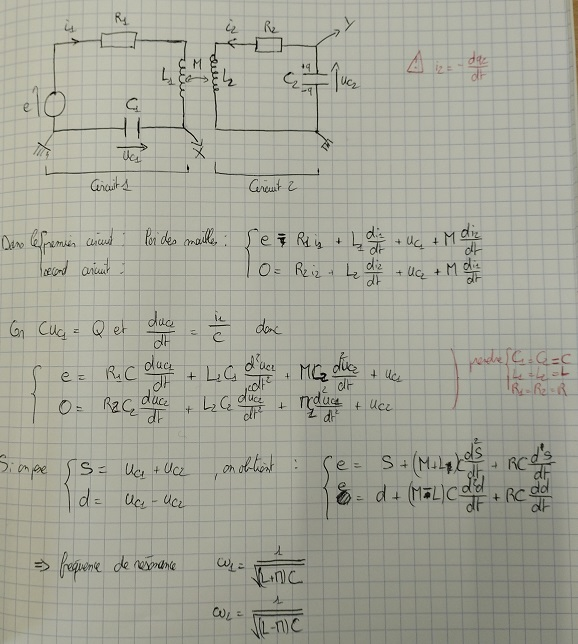
\includegraphics[scale=0.5]{LP_Resonance/Oscillateurs_couple.jpg}
\end{center}    


\textcolor{blue}{Expérience : }montrer l'influence du couplage sur la résonance du premier circuit RLC à l'aide d'un deuxième circuit RLC. Intérêt pratique ?

\section{Cavité résonante}
\subsection{Cavité Fabry Pérot}
\subsection{Intensité transmise}
Calcul possiblement à faire soit hyper rapidement, soit en prérequiss.

\subsection{Finesse}
\end{reportBlock}
\newpage 
%%%%%%%%%%%%%%%%%%%%%%%%%%%%%%%%%%%%%%%%%%%%%%%%%%%%
%%%% En-tête leçon
\begin{headerBlock}
  \chapter{Oscillateurs ; portraits de phase et non-linéarités.}
  \label{LP_PortaitPhase} 
\end{headerBlock}




%%%%%%%%%%%%%%%%%%%%%%%%%%%%%%%%%%%%%%%%%%%%%%%%%%%%
%%%% Références
\begin{center}
\begin{tabularx}{\textwidth}{| X | X | c | c |}
  \hline
  \rowcolor{gray!20}\multicolumn{4}{c}{Bibliographie de la leçon : } \\
  \hline 
  Titre & Auteurs & Editeur (année) & ISBN \\
  \hline
   \url{https://uhincelin.pagesperso-orange.fr/LP49_BUP_portrait_phase_oscil.pdf} & H. Gié &  BUP n°744&    \\
  \hline 
   \url{https://www.lpens.ens.psl.eu/wp-content/uploads/2022/09/MecaniquePourChimistes-3.pdf} & Jules Fillette & &  \\
  \hline 
\end{tabularx}
\end{center}

%%%%%%%%%%%%%%%%%%%%%%%%%%%%%%%%%%%%%%%%%%%%%%%%%%%%

%%%%%%%%%%%%%%%%%%%%%%%%%%%%%%%%%%%%%%%%%%%%%%%%%%%%
%%%% Plan
\begin{reportBlock}{Plan détaillé}

  \textbf{Niveau choisi pour la leçon :} CPGE 2ème année
  \newline
  \textbf{Prérequis} : \begin{itemize}
      \item TMC,
      \item Electrocinétique : schéma électrique, loi des mailles, résistance, condensateur, inductance
  \end{itemize}

  \textbf{Déroulé détaillé de la leçon: }  
  
  \section*{Introduction}
Messages à faire passer : définition d'un portait de phase, portait de phase amorti/non-amorti, stabilité des points fixes, centres attracteurs.\\

Le notion de portait de phase est un outil très riche pour l'analyse de nombreux systèmes mécaniques, en particulier pour les oscillateurs. C'est que nous allons essayer de montrer dans cette leçon à travers quelques exemples.

  \section{Oscillateurs non-amortis}
  On va s'intéresser à des systèmes mécaniques ou électrocinétiques dont on va négliger les phénomènes de dissipation. On va commencer par prendre l'exemple très simple du pendule pesant.
  \subsection{Equation du mouvement d'un pendule pesant}
  Exemple de la physique : pendule simple à petites oscillations. On applique le théorème du moment cinétique appliqué à la masse $m$ dans le référentiel terrestre qu'on suppose galiléen :
  \begin{equation}
     \frac{d\mathbf{L_O}(M)}{dt} = mL^2\ddot{\theta}\mathbf{\hat{u_z}} = \mathbf{M_O}(\mathbf{P}) = -mgLsin(\theta)\mathbf{\hat{u_z}}
  \end{equation}
  On en déduit l'équation d'un oscillateur harmonique de pulsation propre $\omega_0=\sqrt{\frac{g}{L}}$ :
  \begin{equation}
      \ddot{\theta} + \omega_0^2\sin(\theta) = 0
  \end{equation}
  \textbf{Analogies :} courant dans un circuit LC suit la même équation.
  \subsection{Portrait de phase}
  Définition d'un portait de phase.
  \subsection{Approche énergétique}
  Parler de stabilité, conservation de l'énergie mécanique.

  

  \section{Effets non linéaires}
  Formule de borda pendule.\\

  \section*{Conclusion}
  Ouvrir sur les oscillateurs entretenus ? Van der Pol, résistance négative,

  \textcolor{blue}{Manip quanti :} mettre en évidence non linéarités, déterminer formule de Borda.
  


\end{reportBlock}
\newpage
%%%%%%%%%%%%%%%%%%%%%%%%%%%%%%%%%%%%%%%%%%%%%%%%%%%%
%%%% En-tête leçon
\begin{headerBlock}
  \chapter{Cinématique relativiste. Expérience de Michelson et Morlay}
    \label{LP_CinematiqueRelativiste}
\end{headerBlock}

%%%%%%%%%%%%%%%%%%%%%%%%%%%%%%%%%%%%%%%%%%%%%%%%%%%%
%%%% Références
\begin{center}
\begin{tabularx}{\textwidth}{| X | X | c | c |}
  \hline
  \rowcolor{gray!20}\multicolumn{4}{c}{Bibliographie de la leçon : } \\
  \hline 
  Titre & Auteurs & Editeur (année) & ISBN \\
  \hline
  Relativité & M. Boratev et R. Kerner & Ellipses & \\
  \hline
  La relativité & A. Einstein & Payot & \\
  \hline
  Relativité et Invariance - Fondements et applications & J.-P. Pérez & Dunod & \\
  \hline
  Relativité Restreinte (exos) & Y. Simon & Armand Colin & \\
  \hline
  Mécanique 1 (Chap 1) & BFR & Dunod (1984) & \\
  \hline
  \url{http://blog.ac-versailles.fr/profbcasanova/public/TS4_phychim/P8_muons-2014.pdf} & & & \\
  \hline
  Mécanique 1 (Chap 15) & H. Gié et J.-P. Sarmant & Tec\&Doc (1984) & \\
\end{tabularx}
\end{center}

\begin{reportBlock}{Commentaires des années précédentes :}
    \begin{itemize}
        \item \textbf{2016 :} Les notions d’événement et d’invariant sont incontournables dans cette leçon,
        \item \textbf{2015 :} Le jury rappelle qu’il n’est pas forcément nécessaire de mettre en œuvre des vitesses relativistes pour être capable de détecter et de mesurer des effets relativistes,
        \item \textbf{2014 :} Cette leçon exige une grande rigueur dans l’exposé tant sur les notions fondamentales de relativité restreinte que sur les référentiels en jeu. Elle invite les candidats à faire preuve d’une grande pédagogie pour présenter des notions a priori non intuitives et faire ressortir les limites de l’approche classique. Un exposé clair des notions d’invariant relativiste est attendu.
    \end{itemize}
\end{reportBlock}

%%%%%%%%%%%%%%%%%%%%%%%%%%%%%%%%%%%%%%%%%%%%%%%%%%%%
\begin{reportBlock}{Plan détaillé}
  \textbf{Niveau choisi pour la leçon :} L3
  \newline
  \textbf{Prérequis : }
  \newline

\section*{Introduction}

\section{Emergence de la relativité restreinte}

\subsection{Transformation de galilée en électromagnétisme}
Les équations de l'électromagnétisme ne sont valables que dans le référentiel de l'éther pour concilier mécanique classique et électromagnétisme.
\subsection{Expérience de Michelson et Morlay}
Montrer les résultats de l'expérience de Michelson et Morlay (Michelson et Morlay, 1887). 

\subsection{Postulat d'Einstein}

\section{Changement de référentiel relativiste}

\subsection{Evènements}

\subsection{Transformation de Lorentz}

\subsection{Intervalle d'espace-temps}

\section{Conséquences physiques}
\subsection{Dilatation du temps}
\textcolor{blue}{Expérience :} utilisaion du programme Gum\_C pour la détermination de $\gamma$ des muons d'après l'expérience de Frish et Smith.
\subsection{Contraction des longueurs}

\end{reportBlock}
\newpage
%%%%%%%%%%%%%%%%%%%%%%%%%%%%%%%%%%%%%%%%%%%%%%%%%%%%
%%%% En-tête leçon
\begin{headerBlock}
  \chapter{Effet tunnel. Application à la radioactivité alpha.}
    \label{LP_EffetTunnel}
\end{headerBlock}

%%%%%%%%%%%%%%%%%%%%%%%%%%%%%%%%%%%%%%%%%%%%%%%%%%%%
%%%% Références
\begin{center}
\begin{tabularx}{\textwidth}{| X | X | c | c |}
  \hline
  \rowcolor{gray!20}\multicolumn{4}{c}{Bibliographie de la leçon : } \\
  \hline 
  Titre & Auteurs & Editeur (année) & ISBN \\
  \hline
  Reflexion totale frustrée & Polycopié de Jean Hare + Perez EM p581 &  & \\
  \hline
  Tout-en-un PC/PC* & M.-N. Sanz & Dunod & \\
  \hline
  Leçons de Physique & Patrick Charmont & Dunod (2000) & \\
  \hline
  \url{https://cahier-de-prepa.fr/pc*-poincare/download?id=1007} & & & \\
  \hline
\end{tabularx}
\end{center}

%%%%%%%%%%%%%%%%%%%%%%%%%%%%%%%%%%%%%%%%%%%%%%%%%%%%
\begin{reportBlock}{Plan détaillé}
  \textbf{Niveau choisi pour la leçon :} 
  \newline
  \textbf{Prérequis : }
  \begin{itemize}
      \item Postulats de la mécanique quantique
      \item Particule dans un puit de potentiel harmonique
  \end{itemize}

\section*{Introducion}
Les lois de la mécanique quantique sont très différentes de la physique classique. Par exemple, du point de vue classique : si une particule voit un puit de potentiel, elle rebondit si elle n'a pas assez d'énergie. En revanche, la dualité onde-particule de la matière (introduite par de Broglie) va montrer quelques effets intéressants : l'aspect ondulatoire de la matière va permettre la transmission de la particule même si celle-ci possède une énergie inférieure au potentiel : c'est l'effet tunnel.

\textcolor{red}{Décrire le modèle en disant ce qu'on}
\section{Etats liés vs états de diffusion}
\subsection{Fonction d'onde et équation de Schrodinger}

Probabilité : $|\psi(x,t)|^2dx$ = probabilité de trouver la particule entre x et x+dx. Interprétation possible que si $\int_{-\infty}^{+\infty}|\psi(x,t)|^2dx=1$.\\

Equation de Schrodinger : $i\hbar\partialD{\psi(x,t)}{t}=-\frac{\hbar^2}{2m}\partialD{^2\psi(x,t)}{x^2}+V(x)\psi(x,t)$\\

Equation linéaire, on peut choisir $\psi = \chi(x)\exp\left(-\frac{iE}{h}t\right)$ avec le signe - dans l'exponentiel pour faire correspondre l'énergie de la particule.\\

Energie = valeur propre de H, c'est ce qu'on cherche à résoudre tout le temps en mécanique quantique. 
\begin{itemize}
    \item Si V confinement $V\sim x^2$, alors E est quantifié. on a des \textbf{états liés}
    \item Si V non confinement, E est continue et on a des \textbf{états de diffusion (ou libres)}
\end{itemize}

Etats de diffusion : ce sont les états qui vont nous intéresser pour l'effet tunnel. Comment les interpréter ?

\subsection{Courant de probabilité}
Introduire le courant de probabilité et la densité de proba : 
\begin{itemize}
    \item $\rho(x,t)=|\psi(x,t)|^2$ densité de proba
    \item $\mathbf{j}(x,t)=\frac{\hbar}{2m}\left(\psi^*\partialD{\psi}{x}-(\partialD{\psi^*}{x})\psi\right)$, courant de probabilité
\end{itemize}

Dans le cas d'une onde plane (non intégrable): 
\begin{itemize}
    \item onde progressive : $\chi(x)=A\exp\left(ikx\right)$ et $\mathbf{j}(x,t)=\frac{\hbar k}{m}|A|^2\mathbf{e_x}$ courant de proba dans le sens $+\mathbf{e_x}$
    \item onde régressive : $\chi(x)=A\exp\left(-ikx\right)$ et $\mathbf{j}(x,t)=\frac{\hbar k}{m}|A|^2\mathbf{e_x}$ courant de proba dans le sens $-\mathbf{e_x}$
\end{itemize}
Schrödinger : $\partialD{\rho}{t}+\nabla\cdot\mathbf{j}=0$ loi de conservation (démo p34 poly Jean Hare).

\section{Effet tunnel : transmission}

\subsection{Le puit carré modèle intégrable de la barrière de potentiel}
Schéma du problème.\\
\begin{itemize}
    \item $E>V_0$ : état de diffusion, pas forcément super intéressant
    \item $E<V_0$ : état de diffusion possible avec une certaine probabilité : c'est l'effet tunnel !
\end{itemize}
Calcul des fonctions d'ondes dans les zones 1, 2 et 3. Dire que $B_3$ s'annule car pas d'onde provenant de $+\infty$.\\

Donner les conditions aux limites $x=0$ et $x=a$. On obtient 4 équations avec 5 inconnues.



\subsection{Coefficients de réflexion et transmission}
Cf Dunod p1252.

\importantbox{Ne pas faire la résolution complète, ça prend beaucoup trop de temps et ce n'est pas intéressant}

On trouve R et T, on verifie qu'on a bien R+T=1 (conservation de l'énergie). \\

\textcolor{blue}{Manip qualitative : montrer logiciel colorado qu'il y a transmission.}

\subsection{Approximation de la barrière épaisse}
Trouver $\delta$, l'interpréter. Garder l'analogie avec réflexion totale frustrée pour les questions.

\section{Application à la radioactivité alpha}

\subsection{Désintégration alpha}
Découverte de la radioactivité. Montrer carte de la stabilité des noyaux. Radioactivité $\alpha$ = noyaux lourds.
\subsection{Modèle de Gamow}
\textcolor{blue}{Expérience :} Code python simulant Gamow (cf Alexandre).

\subsection{Loi de Geiger-Nutall}
\textcolor{blue}{Manip quanti/quali : faire regression $log(T_{1/2}) = \frac{A}{\sqrt{E}}+B$ en utilisant un tableau de données préconstruit.}

\section*{Conclusion}


\end{reportBlock}
\newpage
\part{Leçons de chimie}

%\vspace*{\stretch{0.5}}
%\begin{center}
 %   \vspace{5cm}
  %  \Huge{\textbf{Leçons de chimie}}
%\end{center}
%\vspace*{\stretch{1}}

\newpage
\begin{changemargin}{-1.5cm}{-0cm}

Code couleur pour les manips :
\begin{center}
\textcolor{green}{Expérience déjà faite, sur laquelle je suis à l'aise}\\
\textcolor{yellow}{Retravailler un geste, l'interprétation de l'expérience}\\
\textcolor{red}{Manip à faire en priorité}\\
\end{center}

\begin{tabularx}{\paperwidth-2cm}{| X | X | c | X |}
  \hline
  \rowcolor{gray!20}\multicolumn{4}{c}{Avancement préparation oraux Leçons Chimie} \\
  \hline 
  Titre de la leçon & Elément imposé & Expérience & Niveau \\
  \hline
  \textbf{De la structure à la polarité d'une entité} & logiciel de représentation molécule & \textcolor{red}{\textbf{0\%}}  & 1ère générale - spécialité  \\
  \hline
  \textbf{Evolution d'un système chimique} & Python, déterminer la compo d'un système & \textcolor{red}{\textbf{0\%}}  & 1ère générale - spécialité, Python : cf agreg ou CAPES 2023  \\
  \hline
  \textbf{Dosage} & Dosage par étalonnage (ex: sérum phy) & \textcolor{red}{\textbf{0\%}}  & 1ère générale - spécialité \\
  \hline
  \textbf{Synthèse, traitement, caractérisations} p\pageref{LC_SyntheseTraitement} & Filtration sous vide & Synthèse acide benzoïque  & 1ère générale - spécialité \\
  \hline
  \hline
  \textbf{Oxydants et réducteurs} & Réaliser une pile & \textcolor{green}{Pile Daniell}  & Term générale - spécialité \\
  \hline
  \textbf{Chimie analytique quantitative et fiabilité} & Titrage par conductimétrie & \textcolor{green}{Titrage ions Cl dans sérum phy}  & Term générale - spécialité  \\
  \hline
  \textbf{Evolution spontanée d'un système} & Déterminer $Q_{final}$ & \textcolor{red}{\textbf{0\%}}  & Term générale - spécialité  \\
  \hline
  \textbf{Cinétique et catalyse} & Mise en évidence d'un effet catalyseur & \textcolor{red}{\textbf{0\%}}  & Term générale - spécialité  \\
  \hline
  \textbf{Stratégies en synthèse organique} & Protocole d'optimisation d'un rendement/vitesse & \textcolor{red}{\textbf{0\%}}  & Term générale - spécialité  \\
  \hline
  \hline
   \textbf{Structure spatiale des molécules} & Différencier 2 stéréoisomères & \textcolor{red}{\textbf{0\%}}  & 1ère STL  \\
  \hline
  \textbf{Réactions acide-base en solution acqueuse} & Préparer une solution tampon & \textcolor{red}{\textbf{0\%}}  & 1ère STL  \\
  \hline
  \textbf{Solvants et solubilité} & Etudier facteur influençant la solubilité & \textcolor{red}{\textbf{0\%}}  & 1ère STL  \\
  \hline
  
  
\end{tabularx}
\end{changemargin}
\newpage
\begin{changemargin}{-1.5cm}{0cm}

Code couleur pour les manips :\\
\begin{center}
\textcolor{green}{Expérience déjà faite, sur laquelle je suis à l'aise}\\
\textcolor{yellow}{Retravailler un geste, l'interprétation de l'expérience}\\
\textcolor{red}{Manip à faire en priorité}\\
\end{center}

\begin{tabularx}{\paperwidth-2cm}{| X | X | X | X |}
  \hline
  \rowcolor{gray!20}\multicolumn{4}{c}{Avancement préparation oraux Leçons Chimie} \\
  \hline 
  Titre de la leçon & Elément imposé & Expérience & Niveau \\
  \hline
  \textbf{Synthèse, purification, contrôle pureté liquide organique} & CCM & \textcolor{red}{\textbf{0\%}}  & 1ère SPCL  \\
  \hline
  \textbf{Réactivité des alcools} & Recristallisation & \textcolor{green}{Aspirine}  & 1ère SPCL  \\
  \hline
  \textbf{Réactions de synthèse, sites electrophiles, nucléophiles, formalisme flèches courbes} & Montage à reflux & \textcolor{red}{\textbf{0\%}}  & 1ère SPCL \\
  \hline
  \textbf{Stéréochimie de configuration}, p\pageref{LC_Stéréochimie} & Différencier 2 stéréoisomères & \textcolor{red}{Hydro-halogénation régiosélective}  & Terminale SPCL \\
  \hline
  \textbf{Distillation et diagrammes binaires}, p\pageref{LC_Distillation} & Distillation & \textcolor{green}{Distillation eau-éthanol}  & Terminale SPCL \\
  \hline
   \textbf{Techniques spectroscopiques} & Déterminer C d'après une courbe d'étallonnage & \textcolor{green}{Dosage bleu brillant dans le curaçao}  & Terminale SPCL \\
  \hline
  \textbf{Conductivité} & Titrage par précipitation & \textcolor{green}{Déterminer concentration Cl dans le sérum phy}  & Terminale SPCL, revoir plan pour caler les expériences\\
  \hline
  \textbf{Solubilité} & Extraire sélectivement les ions d'un mélange & \textcolor{green}{Extraction sélective des ions fer dans une solution de nitrate de fer et de sulfate de cuivre (Mesplède p193)}  & Terminale SPCL \\
  \hline
  \textbf{Oxydoréduction} & Titrage dont la réaction support est une oxydo-reduction & \textcolor{green}{Titrage des ions hypochlorite contenus dans le Dakin/eau de Javel}  & Terminale SPCL \\
  \hline
  \textbf{Réactivité des dérivés d'acide} & Montage Dean-Stark & \textcolor{green}{Synthèse arôme de banane}  & Terminale SPCL \\
  \hline
  \textbf{Electrolyse, électrosynthèse} & Réaliser une électrolyse à anode soluble & \textcolor{red}{Elec à anode soluble}- Florence Porteu-de-Buchère - Dunod p190 & Terminale SPCL \\
  \hline
\end{tabularx}
\end{changemargin}

\newpage
\begin{changemargin}{-1.5cm}{-0cm}
    
\begin{tabularx}{\paperwidth-2cm}{| X | X | X | X |}
  \hline
  \rowcolor{gray!20}\multicolumn{4}{c}{Avancement préparation oraux Leçons Chimie} \\
  \hline 
  Titre de la leçon & Elément imposé & Expérience & Niveau \\
  \hline
  \textbf{Energie chimique - exemple des combustions} & Estimer pouvoir calo d'une combustion & \textcolor{green}{Voir Nathan ST2S}  & 1ère/terminale STI2D \\
  \hline
  \textbf{Oxydoréduction} p\pageref{LC_Oxydoreduction_STI2D} & Déterminer la capacité d'un accumulateur & \textcolor{red}{Accumulateur au plomb}  & 1ère/terminale STI2D \\
   \hline  
  \hline
  \textbf{Molécules d'intérêt biologique} & Différencier aldéhyde/cétone & \textcolor{green}{Voir Nathan ST2S} & 1ère ST2S \\
  \hline
  \textbf{Gestion des risques au laboratoire de chimie} p\pageref{LC_GestionRisquesLabo} & Mettre en \oe uvre un protocol de neutralisation & \textcolor{green}{Neutralisation acide} & 1ère ST2S \\
  \hline
   \textbf{Biomolécules et énergie} p\pageref{LC_BiomoleculesEnergie} & Réaliser l'hydrolyse d'un glucide complexe & \textcolor{green}{Voir Nathan ST2S}  & 1ère ST2S \\
  \hline 
  \textbf{L'eau, propriétés physiques et chimiques} & Réaction une extraction liquide/liquide & \textcolor{red}{0\%} & 1ère ST2S \\
  \hline 
  \hline
  \textbf{Chimie et alimentation} & Teneur en vitamine C d'un aliment/médicament & \textcolor{red}{0\%} & Terminale ST2S \\
  \hline
  \hline
  \textbf{Transformations chimiques en solution acqueuse} & Déterminer $K_{eq}$ d'une réaction (A/B, précipitation, redox) & \textcolor{red}{0\%} & MPSI \\
  \hline
  \textbf{Acides et bases} & Déterminer $K_a$ & \textcolor{red}{0\%} & MPSI \\
  \hline
  \textbf{Solvants} & Déterminer constante de partage & \textcolor{red}{0\%} & MPSI \\
  \hline
  \textbf{Structure et prop des solides} & Utiliser avogadro ou vesta et déterminer des paramètres géométriques & \textcolor{red}{0\%} & MPSI \\
  \hline
  \textbf{Cinétique homogène} & Déterminer $E_a$ & \textcolor{red}{hydrolyse du chlorure de tertiobutyle suivie par pH-métrie} - F. Porteu de Buchère p40& MPSI \\
  \hline
  \textbf{Diagrammes E-pH} p\pageref{LC_DiagrammeEpH} & Mettre en \oe uvre une médiamutation & \textcolor{red}{0\%} & MPSI \\
  \hline
  \textbf{Liaisons chimiques} & Utiliser Vesta ou avogadro & \textcolor{red}{0\%} & MPSI \\
  \hline
\end{tabularx}
\end{changemargin}

\newpage
\begin{changemargin}{-1.5cm}{-0cm}
Code couleur pour les manips :\\
\begin{center}
\textcolor{green}{Expérience déjà faite, sur laquelle je suis à l'aise}\\
\textcolor{yellow}{Retravailler un geste, l'interprétation de l'expérience}\\
\textcolor{red}{Manip à faire en priorité}\\
\end{center}

\begin{tabularx}{\paperwidth-2cm}{| X | X | X | X |}
  \hline
  \rowcolor{gray!20}\multicolumn{4}{c}{Avancement préparation oraux Leçons Chimie} \\
  \hline 
  Titre de la leçon & Elément imposé & Expérience & Niveau \\
  \hline
  \textbf{Utilisation 1er principe pour la détermination de grandeurs physico-chimiques} & Déterminer $\Delta_rH_{reaction}$ & \textcolor{red}{pas fait} - F. Porteu p75 & PSI \\
  \hline
  \textbf{Optimisation d'un procédé chimique} & Mettre en évidence influence T ou P ou catalyseur sur une réaction & \textcolor{red}{0\%} & PSI \\
  \hline
  \textbf{Corrosion humide des métaux} & Protection contre la corrosion (clou+gel agar-agar) & \textcolor{red}{Passivation du fer}-Cachau Redox & PSI \\
  \hline
  \textbf{Générateurs électrochimiques} & Montrer influence de facteurs sur $e_{vide}$ d'une pile & \textcolor{red}{0\%} & PSI \\
  \hline
  \textbf{Conversion d'énergie électrique en énergie chimique} & Déterminer $\eta_{faradique}$ d'un électrolyseur & \textcolor{red}{0\%} & PSI \\
  \hline
  \textbf{Cinétique électrochimique} & Tracer courbe i-E & \textcolor{red}{0\%} & PSI \\
  \hline
  \textbf{Application 2nd principe à une transfo chimique} & Déterminer une constante d'équilibre thermo & \textcolor{red}{0\%} & PSI \\
  \hline
  \hline
  \textbf{Diagramme E-pH} & Réaliser un procédé industriel à l'échelle du labo & \textcolor{red}{0\%} & TSI 2 \\
  \hline
  \textbf{Déplacement de l'équilibre chimique} & Utiliser un bain thermostaté & \textcolor{red}{0\%} & TSI 2 \\
  \hline  
\end{tabularx}

\begin{headerBlock}
\begin{itemize}
    \item Réaliser l'hydrolyse d'un complexe (leçon biomolécules et énergie - 1ère ST2S)
    \item 
\end{itemize}

\end{headerBlock}
\end{changemargin}


\newpage
\begin{headerBlock}
\chapter{L'eau, propriétés physiques et chimiques}
\label{LC_Eau}
 \end{headerBlock}

%%%%%%%%%%%%%%%%%%%%%%%%%%%%%%%%%%%%%%%%%%%%%%%%%%%%
%%%% Références


%%%%%%%%%%%%%%%%%%%%%%%%%%%%%%%%%%%%%%%%%%%%%%%%%%%%
%%%% Plan
\begin{reportBlock}{Bibliographie}

\begin{center}
\begin{tabular}{|c|c|c|c|}\hline
Titre & Auteur(s) & Editeur (année) & ISBN \\ \hline
BUP n$^0$790 ~ & ~ & ~ & ~ \\
\hline
\end{tabular}
\end{center}

\end{reportBlock}

\begin{reportBlock}{Plan détaillé}

\underline{Niveau} : 1èr ST2S \\

\section*{Introduction pédagogique}


\paragraph*{Prérequis}
\begin{itemize}
\item Barycentre
\item Formules développées et semi-développées
\end{itemize}

\paragraph*{Contexte :}
Place de la leçon : milieu d'année.

\paragraph*{Notions importantes}

\begin{itemize}
\item Constante de solubilité
\item sens de l'évolution
\item influence de la solubilité (T, pH, etc...)
\item protocole 
\end{itemize}

\paragraph*{Objectifs}

\begin{itemize}
\item prédire la précipitation, dissolution
\item déterminer la solubilité et prévoir son évolution
\end{itemize}

\paragraph*{Difficultés}

\begin{itemize}
\item Appréhender le caractère polaire/apolaire liée à la géométrie
\item distinctions entre liaisons covalente et hydrogène
\item miscibilité, solubilité
\end{itemize}
Pour y remédier, activité préliminiaire pour manipuler les grandeurs
\section*{Introduction }
Dissolution courante dans la vie de tous les jours.\\
\textbf{Question:}

\paragraph*{Manipulation qualitative:} \textcolor{green}{}

\section{Electronégativité}

\subsection{Liaison polarisée}

\textcolor{red}{Def électronégativité : }Grandeur sans dimension caractérisant la capacité qu'à un atome engagé dans une liaison à attirer les électrons vers lui.\\
Tableau périodique : $\chi(O)>\chi(H)$.\\

\textcolor{red}{Def charge partielle : }$\delta^{\pm}$

\textcolor{red}{Def polarisation d'une liaison chimique : }si $\Delta\chi=0$ : liaison apolaire. si $\Delta\chi\neq 0$ : liaison polaire.

\subsection{La liaison hydrogène}
\textcolor{red}{Def liaison hydrogène : }liaison de type attractive entre deux entités polaires. $E_{liaison-H}=$qqkJ/mol. C'est une liaison électrostatique attractive entre deux charges partielles de signes opposés. Permet d'expliquer, en partie, les différences de température d'ébullition entres des corps purs.


\section{Propriétés chimiques de l'eau}

\textcolor{green}{Manipulation : dépollution de l'eau :} mélange d'eau et de I$_2$ pour faire passer $I_2$ de l'eau au cyclohexane. Puis extraction liquide-liquide avec une ampoule à décanter.

\section*{Conclusion} 
\end{reportBlock}
\newpage
\begin{headerBlock}
\chapter{Solubilité}
\label{LC_Solubilité}
 \end{headerBlock}

%%%%%%%%%%%%%%%%%%%%%%%%%%%%%%%%%%%%%%%%%%%%%%%%%%%%
%%%% Références


%%%%%%%%%%%%%%%%%%%%%%%%%%%%%%%%%%%%%%%%%%%%%%%%%%%%
%%%% Plan
\begin{reportBlock}{Bibliographie}

\begin{center}
\begin{tabularx}{\textwidth}{| X | X | c | c |}\hline
Titre & Auteur(s) & Editeur (année) & ISBN \\ \hline
100 manipulations de chimie (p193)~ & Jacques Mesplède, Jérôme Randon ~ & Bréal (2004) ~ & ~ \\
\hline
\url{http://je-plante-mon-agreg.com/Documents/Chimie_exp\%C3\%A9rimentale-Listes_TP_chimie.pdf} &  &  ~ & ~ \\ \hline
 \url{https://spcl.ac-montpellier.fr/moodle/pluginfile.php/11573/mod_resource/content/2/Chapitre\%201\%20-\%20Solubilite\%20-\%20\%20Fiche\%20de\%20synthese.pdf} & ~ &  & ~ \\ 
 \hline
 \url{http://leonardvinci.e-monsite.com/medias/files/02.solubilite.pdf} & ~ &  & ~ \\ 
 \hline
\end{tabularx}
\end{center}

\end{reportBlock}

\begin{reportBlock}{Plan détaillé}

\underline{Niveau} : Tle STL - SPCL \\

\section*{Introduction pédagogique}


\paragraph*{Prérequis}
\begin{itemize}
\item pH, pH-métrie
\item quantité de matière, masse volumique, concentrations
\end{itemize}

\paragraph*{Contexte :}
Place de la leçon : début d'année.

\paragraph*{Notions importantes}

\begin{itemize}
\item Constante de solubilité
\item prédire l'évolution
\item influence de la solubilité (T, pH, etc...)
\end{itemize}

\paragraph*{Objectifs}

\begin{itemize}
\item prédire la précipitation, dissolution
\item déterminer la solubilité et prévoir son évolution
\end{itemize}

\paragraph*{Difficultés}

\begin{itemize}
\item Difficultés mathématiques (unités, etc...)
\item Lien entre constante d'équilibre et pH
\end{itemize}
Pour y remédier, activité préliminiaire pour manipuler les grandeurs
\section*{Introduction }
Dissolution courante dans la vie de tous les jours. Ex : sucre dans le café.\\
\paragraph*{Manipulation qualitative:} \textcolor{green}{Exp qualitative : mettre du sel dans l'eau}. Quelle est la quantité max de sel qu'on peut mettre dans l'eau ?

\section{Solubilité et produit de solubilité}

\subsection{Solubilité}

\textcolor{red}{Def solubilité : }Notée s, quantité de matière/masse maximale d'une espèce que l'on peut dissoudre dans un litre de solvant (en $mol.L^{-1}$ ou $g.L^{-1}$)\\
ex: s(NaCl)=358.5g.L$^{-1}$ à 20°C.

\subsection{Produit de solubilité}
Pour la réaction : NaCl(s) = Na$^+$(aq) + Cl$^-$(aq)

\begin{equation}
    K_s = \frac{[Na^+]_{eq}[Cl^-]_{eq}}{(C^{0})^2}
    \end{equation}

Tableau d'avancement : $s=\sqrt{K_s}$

\section{Quotient de réaction}

\begin{equation}
    Q_r = \frac{[Na^+]_{eq}[Cl^-]_{eq}}{(C^{0})^2}
\end{equation}
\begin{itemize}
    \item $Q_r<K_s$ : sens direct : dissolution
    \item $Q_r=K_s$ : équilibre
    \item  $Q_r>K_s$ : sens indirect : precipitation
\end{itemize}
\section{Facteurs influençant sur la solubilité}
\subsection{Le pH}
\textcolor{red}{Rappel :} $pH = -\log([H_3O^+])$ \\
Le pH influe sur la solubilité $s$ : Fe(OH)$_3$(s) = Fe$^{3+}$(aq) + 3HO$^-$(aq).
\begin{equation}
    K_s = \frac{[Fe^{3+}]_{eq}[HO^-]_{eq}^3}{(C^{0})^4}
\end{equation}

\textcolor{blue}{Contexte :} application industrielle pour séparer les ions métalliques d'un minerai par exemple.\\
\textcolor{green}{Manipulation principale :} On va mélanger deux solutions à 1M, une solution de sulfate de cuivre (de couleur bleue) et une solution de nitrate de fer (de couleur orange).\\ %schéma expérimental à mettre
On va faire précipiter d'abord les ions fer Fe$^{2+}$ avec une solution de soude à 1M puis filtrer le précipité sur fritté.\\
Les réaction possibles sont :
\begin{itemize}
    \item Fe(OH)$_2$(s) = Fe$^{2+}$(aq) + 2HO$^-$(aq) possible à $pH\sim2$
    \item Cu(OH)$_2$(s) = Cu$^{2+}$(aq) + 2HO$^-$(aq) possible à pH$\sim 4.8$
\end{itemize}
C'est pour ça qu'on utilise un pH-mètre pour contrôler qu'on ne dépasse pas un pH d'environ 4.\\
La manip fonctionne bien, on voit que la couleur de la solution redevient bleue après filtrage du précipité de Fe(OH)$_2$(s).
\subsection{Température}
En général, la solubilité augmente avec la température.\\
\textcolor{red}{Attention : } Il y a des exceptions. $s$ peut diminuer avec la température (ex: calcaire dans la bouilloire).


\section{Conclusion} 
Applications : dépollution de l'eau, séparation des métaux, décalcairisation en milieu acide.

\end{reportBlock}

\begin{reportBlock}{Questions posées}

\begin{itemize}

\item Slide intro, je suis d'accord sur la position de leçon, obectifs : première capacité expérimentale du BO pas mentionnée ? \textcolor{purple}{Non, mais je la travaillerai en TP en demi-groupe.} Quelle technique peut-on utiliser pour extraire le solide ? \textcolor{purple}{Extraction liquide-liquide.}

\item Est-ce que l'appareil de l'extraction a déjà été  vu ? \textcolor{purple}{Je ne me rappelle plus s'ils l'ont vu l'année dernière, mais je ferai une séance d'intro de la verrerie en début d'année. Donc à mettre en préréquis.}

\item Le point à $1mL$ dévie de la droite, pourquoi ? \textcolor{purple}{Cela peut être dû au fait qu'à ce volume, on n'est pas forcément dans le régime linéaire de la loi de Kohlrausch.}

\item Vous donner comme exemple le titrage des ions nitrate. Comment proposez-vous d'en déterminer la concentration ? \textcolor{purple}{En réalisant le même titrage que pour les ions chlorure.} Peut-on dans ce cas déterminer séparément la concentration des 2 analytes (\ce{NO_3^-} et \ce{Cl^-}) ? \textcolor{purple}{Non.}

\item Tu n'as pas du tout parlé de quantité de matière, concentration, etc... ? \textcolor{purple}{J'ai oublié de faire un calcul de la solubilité dans la leçon...} 

\item Pas de problème de vocabulaire sur les difficultés ? C'est quoi un précipité si tu devais le présenter à tes élèves ? \textcolor{purple}{Un solide qui refuse de se dissoudre dans un solvant} 

\item Dans ton expérience introductive, est-ce qu'il reste du sel ? \textcolor{purple}{Quasiment pas, mais j'aurais du utiliser un autre solide coloré pour que ça soit visible (PbI$_2$) par exemple.}

\item Dans la définition de la solubilité, tu as oublié la température. \textcolor{purple}{Oui...}

\item Qu'est-ce qu'il se passe à K$_s$ ? \textcolor{purple}{Il y a coexistence du précipité et des ions en solutions.}

\item Différence entre un état final et un état d'équilibre ? \textcolor{purple}{Oui, il y a une différence. }

\item Peut-on définir K$_s$ pour d'autres composés que ioniques ? \textcolor{purple}{Non, on peut avoir dissolution d'un gaz dans l'eau par exemple.} Que se passe-t'il si P augmmente ? \textcolor{purple}{s augmente}

\item D'autres moyen pour faire varier la solubilité ? \textcolor{purple}{Effet d'ions communs.} 

\item Comment as-tu défini la solution saturée ? \textcolor{purple}{Quand on a ajouté $s$ ou plus de solide dans le solvant.}

\item Lien entre pH et concentration en HO$^-$ ?
\textcolor{purple}{$[HO^-]=10^{-14-pH}$}

\item Comment on fait en pratique pour les minerais ? \textcolor{purple}{Lixiviation, on se place à un pH super acide et on broit les minerais.}

\item Pour la manip, tu voulais faire qualitatif ou quantitatif ?  \textcolor{purple}{Qualitatif.}Comment tu aurais fait pour la rendre quantitatif ? Peux-tu faire le calcul du pH d'apparition de Fe(OH)$_2$(s) ? \textcolor{purple}{$[HO^-]=(\frac{K_s}{[Fe^{2+}]})^{1/3}$. Avec [Fe$^{2+}$]=0.25mol.L$^{-1}$ environ (rajout d'environ le double d'eau du mélange de solution de 10mL de chaque réactif. On trouve $pH=1,87$.} Il aurait fallu faire ce calcul qui est abordable en terminale. Cela aurait permi de mieux comprendre pourquoi on ne devait pas dépasser ce pH.

\item Si tu devais refaire faire la manip aux étudiants, que dirais-tu niveau sécurité pour la fiole à vide ? \textcolor{purple}{Il faut l'attacher avec une pince 3 doigts et une potence.}

\item Pourquoi dans le cas du calcaire c'est une exception ? \textcolor{purple}{Si on augmente la température, la solubilité du CO$_2$ dans l'eau diminue ce qui augmente le pH. }

\item Que proposez-vous en séance de travaux pratiques ? \textcolor{purple}{Le titrage du sérum physiologique, c'est pédagogique car c'est un produit du quotidien.}

\item 
\textcolor{purple}{}

\end{itemize}


\end{reportBlock}

\begin{reportBlock}{Commentaires}
Plan très bien, explications sont claires et pédagogiques. Choix de la manip impecc. Il manque le quantitatif dans la manip. Gestes pour la manip très bien.

\end{reportBlock}


\begin{reportBlock}{Expérience 1}
% bloc à dupliquer autant de fois que d'expériences

\underline{Titre} : Illustration solubilité du sel dans l'eau. \\

\underline{Référence complète} : \\ 

\underline{But de la manip} :En faible quantité ajouté dans l'eau, le sel se dissous complètement. Au-delà d'une certaine concentration de sel, il reste du précipité.\\

\underline{Commentaire éventuel} :On peut faire la manip avec une espèce coloré comme PbI$_2$ pour que ça soit plus visuel.

\underline{Durée de la manip} : 2' \\

\end{reportBlock}



\begin{reportBlock}{Expérience 2}
% bloc à dupliquer autant de fois que d'expériences

\underline{Titre} : Extraction sélective des ions fer dans une solution de nitrate de fer et de sulfate de cuivre. \\

\underline{Référence complète} : 100 manipulations de chimie, J. Mesplède et J. Randon, p193 \\ 

\underline{Équation chimique et but de la manip} : Fe(OH)$_2$(s) = Fe$^{2+}$(aq) + 2HO$^-$(aq) \\

\underline{Phase présentée au jury} : Précipitation des ions fer en maintenant le pH en-dessous de 4. Puis filtration sur fritté. \\

\underline{Commentaire éventuel} : Prévoir un fritté très fin.\\

\underline{Durée de la manip} : 10'\\

\end{reportBlock}

\begin{reportBlock}{Compétence \og Autour des valeurs de la République et des thématiques relevant de la laïcité et de la citoyenneté \fg{}}

\underline{Question posée} : En quoi la démarche scientifique fais de nous des bons citoyens ? \\

\underline{Réponse proposée} : La démarche scientfique c'est : observer de l'environnement, vérifier, raisonner, garder confiance en soi et avoir foi en les autres, être opimiste. Avoir un esprit critique sur des sujets de société. Beaucoup de complotisme de nos jours, la démarche scientifique permet de démonter cela.\\

\underline{Commentaire du correcteur} : 

\end{reportBlock}


\begin{reportBlock}{Champ libre pour le correcteur}
% compléments, propositions de manipulation, bibliographie etc.

\end{reportBlock}
\newpage
%%%% En-tête leçon
\begin{headerBlock}
\chapter{Distillation}
    \label{LC_Distillation}
\end{headerBlock}




%%%%%%%%%%%%%%%%%%%%%%%%%%%%%%%%%%%%%%%%%%%%%%%%%%%%
%%%% Références
\begin{reportBlock}{Bibliographie}

\begin{center}
\begin{tabular}{|c|c|c|c|}\hline
Titre & Auteur(s) & Editeur (année) & ISBN \\ \hline
Tout-en-un Chimie PC/PC* ~ & B. Fosset, J-B. Baudin  ~ & Dunod (2022)~ & ~ \\
\hline 
\url{http://vle-calc.com/} & Site sympa pour les diagrammes ~ &  ~ & ~ \\
\hline
\url{https://spcl.ac-montpellier.fr/moodle/course/view.php?id=61&section=7} & Académie de Montpellier & Eduscol & ~ \\ \hline
\end{tabular}
\end{center}

\end{reportBlock}

%%%%%%%%%%%%%%%%%%%%%%%%%%%%%%%%%%%%%%%%%%%%%%%%%%%%
%%%% Plan
\begin{reportBlock}{Rappels de définitions, concepts à aborder lors de la leçon : }
\textbf{Rappels : } cf le BO de la spécialité SPCL de STL.

\begin{enumerate}
    \item Pouvez-vous rappelez les difficultés associées à cette leçon ? \textcolor{red}{Lecture et compréhension de diagramme binaire, lien avec la distillation, courbe d'analyse thermique (mélange binaire), nombreuses définitions avec lesquelles on joue (fraction molaire/massique/titre/masse molaire, etc...), verrerie associée au montage}. Y-a-t’il une difficulté en terme de vocabulaire ? \textcolor{red}{Clairement, on doit insister sur les définitions et les différents noms de la verrerie spécifique à la distillation} Comment s’appelle le ballon ? \textcolor{red}{Le ballon est un bon exemple pour insister sur les définitions. On le nomme "bouilleur".} C’est un terme qu’on utilise dans d’autres situations ? \textcolor{red}{Dans les chaufferies, sert à faire bouillir le fluide chauffant. Dans l'industrie du sel, présent dans le processus de déssalement.}
    \item L'hydrodistillation est-elle au programme de terminale STL-SPCL ? \textcolor{red}{Oui, dans le thème « Chimie et développement durable ».}
    \item Diagramme binaire, notion théorique ou expérimentale ? \textcolor{red}{C'est une notion théorique à connotation fortement expérimentale car très utile pour déterminer les fractions massiques d'un mélange. Notion théorique car c'est applicable en théorique à tous les mélanges binaires et relié aux concepts thermodynamique (capacité thermique, température de changement d'état donc enthalpie de changement d'état, équation d'état, principes de la thermodynamique, etc...).}
      
\end{enumerate}

\end{reportBlock}

\begin{reportBlock}{Avis sur le plan proposé, choix des exemples et des expériences : }
\textbf{Plan :}\\
\section{Mélanges binaires homogènes}
Pour étudier les mélanges binaires homogènes, on a avoir besoin d'un certains nombre de définitions qui seront importantes dans tout le déroulé de la leçon.
\subsection{Mélange binaire}
Définition d'un mélange homogène : mélange dont on ne peut distinguer à l'\oe il nu ses différents constituants.
Définition d'un corps pur : matière qui ne comporte qu'une espèce chimique.
\subsection{Fraction molaire}
Définition fraction molaire d'un mélange A+B : la fraction molaire d'un corps A est : $x_{A}=\frac{n_A}{n_A+n_B}$, avec $n_i$ la quantité de matière du corps $i$
\subsection{Fraction massique}
Définition fraction massique d'un mélange A+B : la fraction massique d'un corps A est : $w_{A}=\frac{m_A}{m_A+m_B}$, avec m$_i$ la masse du corps $i$.
\section{Diagrammes binaires}
\subsection{Diagramme liquide-vapeur isobare}
Présentation et explication des graphes T=f(x ou w) : on montre la courbe de rosée et la courbe d'ébullition à une pression donnée. On décrit l'exemple particulier du diagramme eau/éthanol.
\subsection{Courbes d'analyse thermique}
Tracé des graphes T(t) pour un corps pur : on part de la phase liquide, on arrive à la température d'ébullition qui marque un pallier jusqu'à ce que la dernière goutte de liquide disparaisse puis elle réaugmente dans la phase gazeuse.\\
Pour un mélange binaire homogène, le plateau de température n'est pas constant car les corps A et B du mélange ont des températures de fusion différentes.\\ 
Définition de corps volatil : on appelle de volatil la capacité d'un solide ou d'un liquide à se vaporiser facilement. On va jouer sur les différences de volatilité entre les corps d'un mélange homogène pour réaliser une distillation par exemple.
\subsection{Azéotrope}
Definition azéotrope : mélange présentant une composition particulière pour lequel il se comporte comme un corps pur (phases L et V à l'équilibre ont la même composition). On le montre explicitement sur le diagramme binaire.
\subsection{Exploitation}
On prend un exemple en se plaçant à une certaine fraction molaire (ou massique) d'un mélange à une température ou le mélange est liquide. On fait la lecture des températures d'ébullition et de condensation. On parle de la composition des premières vapeurs (ou des premières gouttes). On rappelle les propriétés de volatilité des corps, et on fait un exemple sur une seule recondensation en présentant la nature du distillat obtenu.
\section{Application à la distillation}
\subsection{Distillation simple}
Sur slide : rappel du montage, lecture sur le diagramme. Ce montage a déjà été vu dans les cours de première et on va voir un nouveau montage qui est celui de la distillation fractionnée.
\subsection{Distillation fractionnée}
Sur slide et sur la paillasse : rappel montage, lecture sur le diagramme. On insiste sur les noms de la verrerie : ballon à fond rond, colonne de Vigreux, condenseur, erlenmeyer.\\

\textcolor{green}{\textbf{\underline{Expérience :}}}\\


On procède à l'expérience de distillation fractionnée sur un mélange eau/éthanol en pesant au préalable les masses d'eau et d'éthanol pour voir où on se place dans le diagramme binaire. On fait chauffer le mélange et on attend de voir les premières gouttes dans le distillat.\\
La réaction est assez rapide suivant la hauteur de la colonne de Vigreux (10min en préparation, 5min au cours de la leçon, ça dépend aussi de le composition du mélange au départ). Il faut faire attention à ce que la température du thermomètre placé au niveau du coude \{colonne de Vigreux - condenseur\} ne dépasse pas la température de l'azéotrope, sinon cela veut dire qu'on commence à faire recondenser de l'eau dans le distillat ce qui dégrade la distillation.\\
On détermine de la fraction massique à l'aide d'une courbe d'étallonage masse volumique vs titre alcoolémique. Puis on détermine le rendement donné par : $\eta=\frac{m_{\text{eth,distillat}}}{m_{\text{eth,initial}}}$.
\section*{Conclusion}
Ouverture sur l'application de la distillation dans la pétrochimie : on montre le schéma du distillat pour le pétrole (gaz, fioul, pétrole brut etc...) en expliquant que ces différentes phases correspondent au raffinement (pourcentage de distillation) du pétrole brut.\\

\textbf{Avis:} Bonne leçon globalement, attention à la trace écrite et les sous-parties vides.\\
Bien d’avoir choisi un sytème réel, mais garder eau+éthanol pas « A+B ». Bien pour les prérequis mais pas toujours clair sur ce qui est connu. Le dire dans l’intro péda.\\
Utilisation diagrammes binaires solide-liquide : eau + sel pour abaisser le point de fusion sur les routes.\\
Attention ne pas être trop vague sur les réponses, essayer de bien détailler.\\
L’olive : fond rond = ballon, fond plat = bécher\\
Montage à bien expliquer avec un schéma en direct ou un montage en direct. Attention au vocabulaire (bouilleur, distillat, etc…) .\\
Difficulté, la lecture des graphiques peut ne pas être intuitif. \\
Calorifuger la colonne de vigreux pour augmenter la vitesse de distillation. \\
Incertitudes pas adaptées car faits sur la calculatrice et pas sur tableur.\\
A l’aise à l’oral, bien pour les couleurs, attention dans le langage « j’ai 30s donc je me dépêche », être naturel pour être bien en maîtrise (même si dans la tête c’est pas du tout ça).

\end{reportBlock}

\begin{reportBlock}{Remarques sur des points spécifiques de la leçon: }
\begin{enumerate}
    \item Comment faire le lien entre diagramme binaire isobare et isotherme ? Comment à partir d’un diagramme à un fuseau vous pouvez tracer le diagramme binaire correspondant ? \textcolor{red}{Similaire mais avec courbe d'ébullition en haut et courbe de rosée en bas.}
    \item Titre en alcool, fraction molaire/massique, comment vous les reliez ? Comment l'expliquer aux étudiants ? \textcolor{red}{On peut partir des définitions, par exemple le titre massique $w_A=\frac{m_A}{m_A+m_B}$ et utiliser la relation $m_A=n_A\times M_A$ avec $n_A$ la quantité de matière et $M_A$ la masse molaire du corps A. Ensuite en multipliant en haut en en bas de la fraction par $n_A+n_B$, on voit apparaître les fractions molaires $x_{A/B}=\frac{n_A}{n_A+n_B}$ ce qui donne $w_{A}=\frac{x_AM_A}{x_AM_A+x_BM_B}$. Pour le titre massique, on fait la même chose en remplaçant $m_A = \rho_A V_A$.}
    \item En industrie, quel est l'ordre de grandeur des rendements ? Pour l'éthanol ? \textcolor{red}{En général, ils sont optimisés et donc très bons. L'ordre de grandeur pour l'éthanol est de l'ordre de celui du point azéotrope soit 96.5\% à $P=1$~bar pour la distillation fractionnée.} On peut aller plus loin en pureté ? \textcolor{red}{Oui, mais il faut introduire un troisième corps (le benzène pour l'éthanol) et utiliser les diagrammes ternaires. Le rendement est bien plus élevé (l'éthanol anhydre, utilisé pour des réactions très sensibles à l'eau, contient de l'eau à $50$~ppm selon Wikipédia).}
    \item Quelle différence entre l'hydro-distillation et l’entrainement à la vapeur ? En terme de montage expérimental ? \textcolor{red}{L'entraînement à la vapeur d'eau et l'hydrodistillation sont des procédés d'extraction ou de séparation de certaines substances organiques de l'eau. Ces deux termes n'ont pas la même signification. "Hydrodistillation" désigne la distillation d’un mélange hétérogène d’eau et d’un liquide organique. L'hydrostillation est beaucoup utilisé en parfumerie et utilise la décomposition des réactifs (molécules odorantes d'un composé organique libérées après décomposition de ce composé sous l'effet de la chaleur). "L’entraînement à la vapeur" est applicable aux composés peu ou pas solubles dans l'eau, dotés d'une tension de vapeur assez importante vers les $100$~$^{\circ}$C. L’avantage de cette technique réside en l'abaissement de la température de distillation les composés sont donc entraînés à des températures beaucoup plus basses que leur température d’ébullition, ce qui évite leur décomposition.}
    \item Pourquoi cette leçon est dans le cadre du programme "Systèmes et Procédés" ? \textcolor{red}{Le thème « Systèmes et procédés » a pour objectif d’étudier des systèmes réels en analysant les flux d’information, de matière et d’énergie. Il comporte un sous-thème "transport et transformation des flux de matière" dont l'étude est un élément important pour l’analyse et la compréhension des procédés physico-chimiques comme ceux liés à la distillation}
    \item C’est quoi la physique derrière les diagrammes binaires ? Comment obtenir l’équation des courbes rosée/ébullition ? \textcolor{red}{cf. cours de thermochimie.}
    \item Liquide/vapeur seuls diagrammes ? \textcolor{red}{Diagrammes solide-liquide.} Avec solides/liquides que pouvez-vous expliquer ? \textcolor{red}{Salage des routes, mélange eau+sel a une température de fusion plus basse que celle de l'eau pure.} 
    
    \end{enumerate}

\end{reportBlock}

\begin{reportBlock}{Discussion sur les manipulations présentées au cours du montage(objectifs de l’expérience, phases de manipulations intéressantes, difficultés théoriques et techniques) :}
 \begin{enumerate}
      \item	Vous n'avez pas utilisé de gants ? Quelles sont les précautions à prendre pour votre montage ? \textcolor{red}{Non, l'éthanol n'est pas dangereux, on en boit (avec modération) et on l'utilise couramment avec le gel hydroalcoolique par exemple. En revanche il est très inflammable donc il faut l'éloigner des sources de chaleurs.}
      \item Préciser la position du thermomètre sur le distillat ? \textcolor{red}{Il faut qu'il s situe au niveau du coude entre la partie colonne de vigreux et le réfrigérent. On veut connaître la température de la phase vapeur qui sort de la colonne de vigreux et vérifier qu'elle ne dépasse pas la température de l'azéotrope, sinon on commence à évaporer une phase pure en la phase qu'on ne souhaite pas voir présent dans le distillat.}
      \item Pourquoi avez-vous été surprise sur la rapidité de la distillation ? Si on attend encore plus, qu’est-ce qu’il se passe ? \textcolor{red}{C'était un peu plus rapide que pendant la préparation. Ca peut être un peu critique si on attend trop car on va recondenser l'eau dans le distillat et modifier la pureté de l'éthanol distillé.}
      \item Au niveau sécurité ? Quels conseils aux étudiants pour remplir le chauffe ballon ? \textcolor{red}{On fera attention à la fragilité de la verrerie. On fera attention à ce que l'évaporation ne soit pas complète car on peut endommager les équipements et la verrerie. C'est aussi pour cela qu'on utilise des chariots élévateurs pour empêcher le contact bouilleur-chauffage rapidement si besoin.}
      \item Que faut-il utiliser pour homogénéiser la solution dans votre cas ? \textcolor{red}{Que olive avec la forme adaptée (bombée) pour le ballon.} Que feraient les étudiants ? \textcolor{red}{Probablement ils ne se poseraient pas la question sur la forme de l'olive à choisir.} L’olive c’est le seul outil ? \textcolor{red}{Oui ?} C’est quoi une bonne agitation ? \textcolor{red}{Une agitation qui homogénéise bien la solution et que ne créé pas d'éclaboussures.}
      \item Le thermomètre servait à quoi dans le montage ? \textcolor{red}{A vérifier que le température ne dépassait pas celle du point azéotrope du diagramme binaire eau/éthanol}
      \item Si la distillation est trop lente, comment faire pour l'accélérer ? \textcolor{red}{On peut calorifuger les parois de la colonne.}
      \item Si on revient aux incertitudes sur les masses, est-elle représentative de l’incertitude de l’expérience ? \textcolor{red}{Non, l'incertitude va surtout porter sur les pertes de matières lors des différentes manipulations (transfert d'un récipient à un autre, etc.). Ces incertitudes ne peuvent être qu'estimer à vue d'oeil.}
      \item Quel est l’intérêt de présenter les incertitudes ? \textcolor{red}{Elle est intéressante pour faire comprendre le sens physique qu'il y a derrière, voir la propagation des erreurs (incertitudes sur une fraction, une somme) et pour comparer aux valeurs tabulées dans la littérature (fraction massique de l'azéotrope).}
      
  \end{enumerate}

\end{reportBlock}

\begin{reportBlock}{Propositions de manipulations –Bibliographie :}
\begin{enumerate}
    \item Quel TP vous feriez faire aux étudiants dans cette leçon ? Quels composés vous distilleriez dans ce cours-là ? \textcolor{red}{La même expérience que réalisée ici (distillation d'un mélange eau/éthanol) est intéressante. On peut aussi regarder l'effet de la taille de la colonne de vigreux et aussi faire la comparaison distillation fractionnée/distillation simple.}
    \item Si vous avez le choix, vous aborderiez ces notions comme vous l’avez fait ou autrement ? \textcolor{red}{Une analyse documentaire peut être pertinente : proposer des exemples de distillation utilisant les diagrammes binaires en industrie, faire réfléchir sur des montages possibles. Cela permet de se familiariser avec le vocabulaire.}. Où prendriez-vous les docs pour une analyse documentaire ? \textcolor{red}{Internet, Dunod PC, liens vidéos ludiques, simulation ou animation}. Quelles sont les sources que vous avez utilisées sur les diagrammes binaires ? Que pouvez-vous faire avec VLE-calc ? \textcolor{red}{Tracer des diagrammes binaires liquide-vapeur, obtenir les infos sur les azéotropes, etc.} Pas de références papier ? \textcolor{red}{Dunod PC, techniques expérimentales en chimie, principalement internet.}
\end{enumerate} 
\end{reportBlock}



\begin{reportBlock}{Autour des valeurs de la République et des thématiques relevant de la laïcité et de la citoyenneté :}
 Quelle est la place de l’humour sur la copie et à l’oral sur la relation élève professeur ?\\
 \textcolor{red}{L'humour peut être utilisé mais il faut faire attention à ses limites. L'humour à outrance peut décridibiliser l'autorité et se retourner contre l'enseignant, surtout en début d'année. L'humour pour pointer une difficulté d'un élève en classe ou sur la copie peut être très mal pris par l'élève, à voir évidemment avec son caractère en cours d'année. On ne peut pas rire de tout avec les élèves en classe, mais on peut faire de l'humour avec un élève en particulier à condition de connaître son caractère et de respecter des limites de décence. Un exemple humouristique (par exemple montrer une image des Dupontd dans Tintin qui font des bonds sur la lune main dans la main avec des cheveux colorés pour illustrer la gravitation) peut être attrayant et source de motivation/d'intérêt pour l'élève. L'humour est aussi une question de sujets. }
\end{reportBlock}

\newpage
\begin{headerBlock}
\chapter{Conductimétrie}
\label{LC_Conductimétrie}
 \end{headerBlock}

%%%%%%%%%%%%%%%%%%%%%%%%%%%%%%%%%%%%%%%%%%%%%%%%%%%%
%%%% Références


%%%%%%%%%%%%%%%%%%%%%%%%%%%%%%%%%%%%%%%%%%%%%%%%%%%%
%%%% Plan
\begin{reportBlock}{Bibliographie}

\begin{center}
\begin{tabular}{|c|c|c|c|}\hline
Titre & Auteur(s) & Editeur (année) & ISBN \\ \hline
PC Tout-en-un MPSI ~ & Bruno FOSSET,  ~ & Dunod  ~ & ~ \\
~ & Jean-Bernard BAUDIN, ~ &  ~ & ~ \\
~ & Frédéric LAHITÈTE  ~ &  ~ & ~ \\ \hline
Ressources en ligne & ~ & Eduscol & ~ \\ \hline
\end{tabular}
\end{center}

\end{reportBlock}

\begin{reportBlock}{Plan détaillé}

\underline{Niveau} : Tle STL - SPCL \\

\underline{Pré-requis} :
\begin{itemize}
\item Loi d'Ohm
\item Dosage
\item Solubilité/précipitation
\end{itemize}


\section*{Introduction pédagogique}

Leçon placée en début d'année de terminale.

\paragraph*{Prérequis}
\begin{itemize}
\item Loi d'Ohm
\item Dosage
\item Solubilité / Précipitation
\end{itemize}

\paragraph*{Notions importantes}

\begin{itemize}
\item Conductance/conductimétrie.
\item Electrolyte.
\item Loi de Kohlrausch.
\item Prévoir l'allure de titrage.
\end{itemize}

\paragraph*{Objectifs}

\begin{itemize}
\item Principe du conductimètre.
\item Loi de Kohlrausch.
\item Titrage par conductimétrie.
\end{itemize}

\paragraph*{Difficultés}

\begin{itemize}
\item Beaucoup de grandeurs différentes avec différentes unités : conductance, conductivité (Siemens).
\item Cellule conductimétrique (vs. électrodes connues) et fonctionnement du conductimètre.
\item Ions mobiles qui conduisent en solution.
\item Prévoir l'allure $\sigma(V)$ (méthode du tableau)
\end{itemize}

\section*{Introduction (4'01)}

\textbf{Question:} Quelle est la condition pour qu'une solution conduise le courant ?

\paragraph*{Manipulation qualitative:} Solution d'eau distillée dans laquelle on fait passer le courant d'une pile reliée à une ampoule (ou une LED) : l'ampoule ne s'allume pas. Elle s'allume si on rajoute du sel (cf. exp 1).

\section{Conductance et conductivité}

\subsection{Conductance}

\paragraph*{Electrolyte} Solution capable de conduire le courant en présence d'ions mobiles. \\
ex: eau salée \ce{Na^+} et \ce{Cl^-}.

\paragraph*{Conductance} $G = \frac{1}{U} = \frac{1}{R}$. Unité : $S = \Omega^{-1}$ (Siemens). Cette grandeur n'est pas intrinsèque à la solution.

\subsection{Conductivité}

\paragraph*{Conductivité} Schéma de fonctionnement d'un conductimètre : une cellule de mesure constituée de deux plaques parallèles de surface immergée $S$ et séparées d'une distance $L$. \\

\paragraph*{Conductivité}: $\sigma = \frac{G L}{S}$ en $S.m^{-1}$, avec $S$ la surface d'une plaque de la cellule conductimétrique et $L$ la distance entre les deux plaques.


\subsection{Facteurs d'influence de la conductivité (16')}

\paragraph*{Manipulation: } Mesure de la conductivité de deux solutions (NaCl et KCl) (cf. exp 2). $\sigma(_ce{KCl}) = 10,32~mS.cm^{-1}$ et $\sigma(\ce{KCl}) = 12,17~mS.cm^{-1}$

- $\sigma$ dépend de la nature des ions mobiles. \\
- $\sigma$ dépend de la température.\\
- $\sigma$ dépend de la concentration des ions présents en solution.

\subsection{Loi de Kohlrausch (19')}

Soit $n$ ions présents dans un électrolyte, on a 
\begin{equation}
\sigma(T) = \sum_i z_i \lambda_i^0(T) C_i
\end{equation}
avec : \\
$z_i$ le nombre de charge de l'ion $i$, ex: z(\ce{Na^+}) = 1, z(\ce{Cl^{-1}}) = 1. \\
$C_i$ la concentration de l'ion $i$ en $mol.L^{-1}$  \\
$\lambda_i^0(T)$ la conductivité molaire ionique \color{purple} \underline{à dilution infinie} \color{black} de l'ion $i$ en $S.m^2.mol^{-1}$. Elles sont tabulées à 25°C.


\section{Application : titrage par précipitation (24'50)}
cf. exp 3. \\

$ \ce{Cl^{-1}_{(aq)}} + \ce{Ag^+_{(aq)}} = \ce{AgCl_{(s)}}$ . Constante d'équilibre : $K = \frac{1}{K_s} = 10^{9.8} \gg 1$.

\subsection{Analyse qualitative}

Tableau de réaction qualitatif. Avant l'équivalence : \ce{Na^+} reste constante, \ce{Cl^{-}} diminue, \ce{NO_3^{-}} augmente, \ce{Ag^+} disparaît. Comme $\lambda^0(\ce{Cl^{-1}}) > \lambda^0(\ce{NO_3^{-1}})$, la conductivité diminue. Après l'équivalence: \ce{Na^+} reste constante, \ce{Cl^{-}} a disparu, \ce{NO_3^{-}} augmente, \ce{Ag^+} augmente. Comme $\lambda^0(\ce{Cl^{-1}}) > \lambda^0(\ce{NO_3^{-1}})$, la conductivité augmente.

\subsection{Détermination de la concentration en ions chlorure dans le sérum physiologique}

  %\begin{figure}[!htbp]
  \begin{center}
   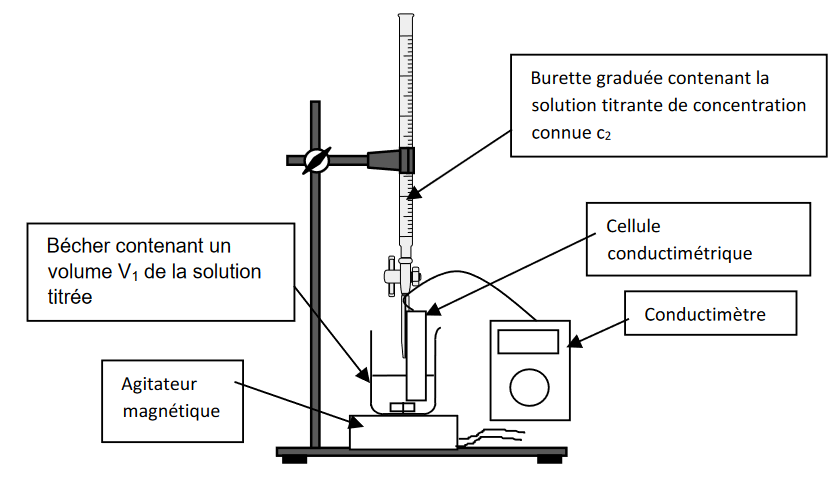
\includegraphics[scale=0.5]{Leçon_chimie/LC_SPCL/LC_Conductimetrie/Schema_titrage.png}
  \end{center}
 
  %\caption{\label{fig:localisation}Schéma de principe du titrage conductimétrique. Le solution titrante est une solution de $AgCl$ à $0.2 mol/L$. La solution titrée est du sérum physiologique.}
  %\end{figure}


Courbe $\sigma(V)$. La détermination du volume équivalent permet de remonter à la concentration des ions Cl$^-$.

\section{Conclusion} Application titrage pour sonder la qualité de l'eau.

\end{reportBlock}

\begin{reportBlock}{Questions posées}

\begin{itemize}

\item Est-ce que c'est important de connaître la valeur du volume d'eau ajouté dans le bécher contenant le réactif titrant lors du titrage conductimétrique ? \textcolor{purple}{Non, ce n'est pas important pour déterminer le volume équivalent lors du titrage.}

\item Pourquoi diluez-vous ?  \textcolor{purple}{Pour pouvoir s'affranchir de la dilution, i.e. obtenir des courbes affines de $\sigma(V)$. Si la solution n'est pas assez dilué on obtient des branches d'hyperbole, qu'on peut corriger en représentant non pas la conductivité $\sigma$ mais la conductivité corrigée $\sigma_{cor}=\sigma \times \frac{V_{tot}}{V_0}$. D'autre part, ça permet d'avoir assez d'eau pour y immerger l'électrode.}

\item Le point à $1mL$ dévie de la droite, pourquoi ? \textcolor{purple}{Cela peut être dû au fait qu'à ce volume, on n'est pas forcément dans le régime linéaire de la loi de Kohlrausch.}

\item Vous donner comme exemple le titrage des ions nitrate. Comment proposez-vous d'en déterminer la concentration ? \textcolor{purple}{En réalisant le même titrage que pour les ions chlorure.} Peut-on dans ce cas déterminer séparément la concentration des 2 analytes (\ce{NO_3^-} et \ce{Cl^-}) ? \textcolor{purple}{Non.}

\item Qu'est-ce qu'on peut chercher d'autre dans l'eau ? Les organismes vivants dans l'eau en ont besoin. \textcolor{purple}{Oxygène.} Comment le titrer ? \textcolor{purple}{Titrage par la méthode de Winkler.} Quels seraient les deux couples en jeu? \textcolor{purple}{Pas si simple. Il y a bien sûr le couple de l'eau faisant intervenir le dioxygène \ce{O_2}/\ce{H_2O} mais aussi des couples du manganèse et de l'iode (voir protocole étudié en TD, diagramme E-pH à l'appui).}

\item Et pour la consommation humaine, que peut-on titrer d'autre? \textcolor{purple}{Les minéraux, comme \ce{Ca^{2+}} ou \ce{Mg^{2+}}.} Pourquoi vouloir déterminer la concentration en ions calcium et magnésium ? \textcolor{purple}{Le calcium peut précipiter avec les ions carbonates CO$_{3}^{2-}$ pour former le carbonate de calcium (c'est-à-dire le calcaire) CaCO$_3$ (qui bouche les canalisations).} Comment les titrer les ions calcium et magnésium ? \textcolor{purple}{Il s'agit d'un titrage complexométrique, le réactif titrant est l'EDTA (éthylènediaminetétracétate), l'indicateur colorée est le NET (pour la dureté totale i.e. $\ce{[Ca^{2+}]+[Mg^{2+}]}$) en tampon ammoniacal à pH 10 et murexide en tampon pH 12 (pour la dureté magnésienne i.e. $[\ce{Mg^{2+}}]$}

\item Peut-on mettre du magnésium métallique dans l'eau ? \textcolor{purple}{Non, c'est un alcalino-terreux et il réagit fortement en présence d'eau.} C'est dangereux ? \textcolor{purple}{Oui, ça s'enflamme.}

\item Comment vous justifiez le choix des doubles flèches dans l'équation de titrage ? \textcolor{purple}{J'aurais dû mettre une flèche simple car c'est une réaction totale dans le sens de la précipitation. À ce propos, voir pour information l'article rédigé par M.Vigneron, X. Bataille et M-B. Mauhourat dans L'Actualité Chimique N°399 de août-septembre 2015 et intitulé \og Du bon usage de la flèche comme symbole de la transformation chimique  \fg{} disponible librement au lien suivant : \url{https://new.societechimiquedefrance.fr/numero/du-bon-usage-de-la-fleche-comme-symbole-de-la-transformation-chimique-p44-n399/}}

\item $\lambda^0$. Que signifie le $0$ ? \textcolor{purple}{Dilution infinie: la loi de Kohlrausch est définie pour des ions infiniment diluées (état hypothétique).}

\item Comment avez-vous étalonné le conductimètre ? \textcolor{purple}{J'ai utilisé une solution étalon \ce{KCl} (chlorure de potassium) pour laquelle on connaît la conductivité en fonction de la température (table de valeurs disponible avec la notice du conductimètre).}

\item Parle-t-on d'électrode en conductimétrie ? \textcolor{purple}{Non, il s'agit d'une cellule conductimétrique.}

\item Pourquoi porter des gants ? \textcolor{purple}{\ce{NaCl} a forte concentration peut-être irritant.} Non, \ce{NaCl} n'est que du sel de cuisine !

\item Quelle est votre politique d'utilisation des gants pour les acides et bases ? \textcolor{purple}{J'en mets dès que la concentration dépasse $10^{-2}$~M.}

\item Pourquoi potassium et sodium ont-ils des conductivités molaires ioniques différentes ? \textcolor{purple}{Taille des noyaux différents et interaction avec les autres ions (VDW, polaire, etc.) différentes. En somme leur rayon de solvatation n'est pas le même.}

\item Sources de la leçon ? \textcolor{purple}{Eduscol, il y a des fiches pour la leçon. Dunod MPSI pour la loi de Kohlrausch. Expérimental: source interne à l'agreg.}

\item Qu'est-ce qui vous a donné l'idée de l'introduction avec la pile ?  \textcolor{purple}{Une source interne à l'agreg (mais ce n'est pas ça qu'il faut dire devant le jury...) Cela a un intérêt pédagogique.}

\item D'après votre introduction pédagogique, les élèves ne connaissent pas la notion de pile. \textcolor{purple}{Je ne pense pas que ça gêne, les élèves manipulent des piles dans leur quotidien.}

\item Quelle est la nature du courant en entrée du conductimètre ? \textcolor{purple}{Un courant alternatif pour éviter de polariser les plaques de la cellule et donc de former un condensateur.}

\item Que proposez-vous en séance de travaux pratiques ? \textcolor{purple}{Le titrage du sérum physiologique, c'est pédagogique car c'est un produit du quotidien.}

\item Comment situez-vous la conductimétrie par rapport à d'autres techniques ? \textcolor{purple}{Je dirais que c'est complémentaire de la pH-métrie par exemple, notamment quand on est dans les conditions d'un saut de pH de faible amplitude qui rend imprécise la détermination de l'équivalence.}

\item Est-ce que ça fonctionne toujours bien ? \textcolor{purple}{Il faut une réaction de titrage thermodynamiquement favorable. Au niveau de l'exploitation, il faut des droites de pentes nettement distinctes pour une détermination aisée et précise du volume équivalent.}

\end{itemize}


\end{reportBlock}

\begin{reportBlock}{Commentaires}

Avoir du matériel en rab au cas où. \\
Attention aux gants lorsque c'est inutile. \\
Intro pédagogique était bien, un peu trop longue. \\
Conductance et conductimétrie pourrait être dans la même partie. \\
Il faut employer le mot "cellule". \\
Tu pourrais utiliser une flexcam pour que le jury voit les valeurs. \\
Tu as donné beaucoup de valeurs de $\lambda_i^0$. Je te conseille de les projeter. \\
J'aurais mis un $=$ à la place des flèches. \\
Prends plus de place pour faire ton tableau. \\
C'est un peu dangereux de mettre l'expérience principale à la fin de la leçon. \\
Rester motiver jusqu'à la fin.


\end{reportBlock}


\begin{reportBlock}{Expérience 1}
% bloc à dupliquer autant de fois que d'expériences

\underline{Titre} : Illustration solution conductrice avec allumage d'une ampoule. \\

\underline{Référence complète} : (référence interne à l'agreg, compte rendu d'une leçon précédente) \\ 

\underline{But de la manip} : montrer que seule la solution d'eau dans laquelle on a ajouté du sel peut allumer l'ampoule : montrer ce qu'est un électrolyte. \\

\underline{Commentaire éventuel} : Attention à brancher la LED dans le bon sens ! Et demander une pile supplémentaire au cas où elle soit déchargée. \\

\underline{Phase présentée au jury} : Circuit ampoule + batterie + deux plaques de cuivre plongées dans une solution. Avec solution = eau distillée : l'ampoule ne s'allume pas. Avec de l'eau salée, l'ampoule s'allume.  \\

\underline{Durée de la manip} : 2' \\

\end{reportBlock}



\begin{reportBlock}{Expérience 2}
% bloc à dupliquer autant de fois que d'expériences

\underline{Titre} : Mesure de la conductivité de deux solutions (NaCl et KCl). \\

\underline{Référence complète} :  \\ 

\underline{Équation chimique et but de la manip} : Montrer que deux électrolytes conduisent différemment. Discuter autour du rayon de solvatation.

\underline{Phase présentée au jury} : Mesure avec un conductimètre de deux solution (NaCl et KCl). \\

\underline{Durée de la manip} : 2' \\

\end{reportBlock}


\begin{reportBlock}{Expérience 3}
% bloc à dupliquer autant de fois que d'expériences

\underline{Titre} : Titrage conductimétrique d'un sérum physiologique \\

\underline{Référence complète} : Hatier, Physique-Chimie Tle spé, 2012, pp.  467-477. \\ 

\underline{Équation chimique et but de la manip} : $ \ce{Cl^{-}_{(aq)}} +\ce{ Ag^+_{(aq)}} = \ce{AgCl_{(s)}}$ \\


\underline{Commentaire éventuel :} Prévoir une deuxième propipette si celle que vous avez est abimée. Par ailleurs, c'est toujours risqué de vouloir ajouté un point au milieu d'une courbe déjà pré-tracée. Ce n'est pas du tout sûr qu'il tombe bien. Mais comme on n'a pas trop le choix au vu de l'exercice demandé, il faut s'y attendre et prévoir de commenter...\\

\underline{Phase présentée au jury} (pendant la séance de question car la manip prévue en fin de leçon n'a pas pu être réalisée par manque de temps) : Prélèvement de la solution titrante de nitrate d'argent à l'aide d'une pipette jaugée (10mL). Ajout de 50~mL d'eau distillée pour avoir suffisamment de solution pour la cellule soit complètement immergée dans la solution à titrer. Mesure d'un point (ajout d'un volume de nitrate d'argent et mesure de la conductivité). Ajouter ce point à la courbe établie lors de la préparation. Commenter si cette valeur est différente de celle attendue dans la courbe (température différente, concentration de la solution différente, etc...)\\

\underline{Durée de la manip} : (de 35'30 - fin) \\

\end{reportBlock}



\begin{reportBlock}{Compétence \og Autour des valeurs de la République et des thématiques relevant de la laïcité et de la citoyenneté \fg{}}

\underline{Question posée} : Qu'est-ce qu'un bon établissement scolaire ? \\

\underline{Réponse proposée} : Il faut d'abord définir ce qu'est un établissement solaire. Matériellement c'est une structure, des salles de classes, du matériel. Un bon établissement est une structure capable de fournir un bon cadre matériel au bon déroulé de l'apprentissage. D'autre part, ce sont des ressources humaines, donc un bon établissement, ce sont des gens qui collaborent bien. Enfin, un bon moyen de reconnaître si un établissement est bon est de suivre le devenir des élèves à la sortie de cet établissement. \\

\underline{Commentaire du correcteur} : Bien. De nombreux mots-clés ont été mobilisés. L'écueil principal de cette question consiste à résume un bon établissement scolaire à un bon pourcentage de réussite au baccalauréat ou d'intégration des filières d'élite. À éviter ! 

\end{reportBlock}


\begin{reportBlock}{Champ libre pour le correcteur}
% compléments, propositions de manipulation, bibliographie etc.

\paragraph*{Remarques sur le plan}
Le plan nécessite d'être revu pour plusieurs raisons. Tout d'abord l'expérience quantitative de titrage du sérum physiologique \textbf{ne tient pas dans le temps imparti} et c'est un problème. De manière générale, il est préférable que l'expérience principale ne soit pas prévue à la fin de la leçon ou au moins qu'elle soit suivie d'une partie tampon que vous pouvez éventuellement supprimer si vous manquez de temps. Dans tous les cas, vous devez avoir l'œil sur votre chronomètre et savoir à quel moment vous avez prévu de passer à la partie ou sous-partie suivante : tout doit être minuté. Une leçon se répète en amont de la présentation, c'est à mettre en place avec votre binôme jusqu'à ce que vous soyez à l'aise.\\

D'autre part, il y a beaucoup \textbf{(trop) de définitions}. Il convient de faire un tri entre celles qui sont les plus importantes et méritent d'être écrites au tableau, celles moins importantes qui peuvent être affichées sur diapositives et celles anecdotiques qu'on peut soit ignorer soit reléguer dans les pré-requis. Par exemple pour la première partie, je propose de renommer ainsi les sous-parties : 1/ Définitions ; 2/ Présentation du conductimètre ; 3/ et 4/ inchangées.\\

\paragraph*{Vocabulaire}
Dans cette leçon il est primordial d'utiliser le bon vocabulaire. Il convient notamment de parler de \textbf{cellule conductimétrique} et non d'électrode, ou encore de faire la distinction entre la \textbf{conductivité ionique molaire et celle à dilution infinie}.\\

\paragraph*{Équipements de protection individuelle}
Vous devez avoir du discernement quant au port des \textbf{gants}. Il est aberrant d'entendre que \ce{NaCl} est une espèce toxique qui nécessite de porter des gants alors que vous l'utilisez quotidiennement en cuisine ! Par ailleurs, assurez vous d'avoir une \textbf{blouse} qui couvre vos bras jusqu'au bout des manches du pull / t-shirt / chemise que vous portez en-dessous.\\

\paragraph*{Autre expérience possible} Si vous envisagez d'illustrer le facteur d'influence qu'est la température, sachez que vous avez à votre disposition des béchers thermostatés. Ce sont des béchers à double paroi qu'on peut relier par des tuyaux (du même type que ceux qu'on utilise pour les réfrigérants) au bain thermostaté. Cependant, il ne faut pas rajouter une expérience supplémentaire à la leçon telle qu'elle à été présenté. Ce serait en remplacement.\\

\paragraph*{Quelle flèche utiliser ?} Pour les équations de réaction en chimie générale, lorsqu'on s'intéresse aux bilans, je vous conseille d'utiliser le signe \og égal \fg{}, même s'il y a précipitation.\\

\paragraph*{Utilisation de la pipette jaugée} Je rappelle la façon correcte de prélever à la pipette jaugée. La pipette doit être tenue verticalement. La main qui tient la pipette (en bas) tient également le bécher (soit de prélèvement, soit celui dans lequel on compte verser la solution prélevée). Le bécher est incliné à 45\degre . L'extrémité inférieure de la pipette (par où s'écoule la solution) est en contact avec la paroi du bécher (immergée si c'est un prélèvement, émergée si l'on est en train de vider la pipette). La seconde main est stabilisatrice en haut de la pipette et manipule la propipette. Lors du prélèvement, il faut toujours dépasser le trait de jauge puis ajuster en descente. La pipette jaugée est une verrerie \og ex \fg{}. Elle est faite pour délivrer le volume indiqué par le constructeur (et non pas pour contenir ce volume, contrairement à la fiole jaugée qui est une verrerie \og in \fg{} ). Dans le cas d'une pipette à 1 trait, peu importe la goutte qui resterait en bas de la pipette une fois celle-ci vidée, le volume est calculé en en tenant compte, à condition qu'elle est été utilisée canoniquement avec ce fameux contact verre-verre permis par l'inclinaison à 45\degre de l'ensemble pipette + bécher. Pour information, la pipette jaugée est calibrée pour prélever une solution aqueuse et perd en précision si elle est utilisée pour prélever un liquide organique.

\end{reportBlock}
\newpage
\begin{headerBlock}
\chapter{Cinétique électrochimique}
\label{LC_CinetiqueElectrochimique}
 \end{headerBlock}

%%%%%%%%%%%%%%%%%%%%%%%%%%%%%%%%%%%%%%%%%%%%%%%%%%%%
%%%% Références


%%%%%%%%%%%%%%%%%%%%%%%%%%%%%%%%%%%%%%%%%%%%%%%%%%%%
%%%% Plan
\begin{reportBlock}{Bibliographie}

\begin{center}
\begin{tabularx}{\textwidth}{| X | X | c | c |}\hline
Titre & Auteur(s) & Editeur (année) & ISBN \\ \hline
 &  &  &  \\ 
 \hline
\end{tabularx}
\end{center}

\end{reportBlock}

\begin{reportBlock}{Plan détaillé}

\underline{Niveau} : PSI \\

\section*{Introduction pédagogique}


\paragraph*{Prérequis}
\begin{itemize}
\item Oxydoréduction
\item Thermochimie
\end{itemize}
\paragraph*{Contexte :}


\paragraph*{Notions importantes}

\begin{itemize}
\item Vitesse de réaction
\end{itemize}

\paragraph*{Objectifs}

\begin{itemize}
\item Tracer une courbe intensité-potentiel
\item déterminer la solubilité et prévoir son évolution
\end{itemize}

\paragraph*{Difficultés}

\begin{itemize}
\item Réaction en milieu hétérogène
\item Pk montage à 3 électrodes
\end{itemize}
Pour y remédier,différencier milieu homogène, milieu hétérogène. 
\section*{Introduction }
Réaction à la surface d'une électrode. On va relier vitesse et thermodynamique.

\section{Réaction électrochimique}

\subsection{Description}
On s'intéresse à l'équilibre :
\begin{equation}
    Red = Ox + ne^-
\end{equation}

Ex : Fe$^{2+}$ = Fe$^{3+}$ + 1 e$^-$. Cette réaction n'a pas de réalité physique car l'électron n'existe pas en solution. En revanche, à la surface d'une électrode métallique, il y a formation d'un électron libre : c'est ce qu'on appelle une réaction électrochimique.

\subsection{Facteur cinétique}
En milieu homogène : 
\begin{itemize}
    \item La proba de renconre entre deux réactifs
    \item La proba que la réaction se produise quand les réactifs sont en contact
\end{itemize}
En milieu hétérogène :
\begin{itemize}
    \item Les réactifs doivent atteindre a surface de l'électrode
    \item le transfert d'électron doit se produire
    \item le produit doit s'éloigner de la surface de l'électrode
\end{itemize}
Schéma (slide) étapes d'une réaction électrochimique.

\subsection{Intensité et vitesse de réaction}
\underline{Rappel :} la vitesse de réaction $v$ est égale à la dérivée temporelle de l'avancement $\xi$.\\
En milieu homogène, on s'intéresse à des vitesses volumiques. Ici, il est plus adéquat de considérer des vitesses surfaciques.\\
\textcolor{green}{définition :} En notant $A$ la surface immergée de l'électrode : 
\begin{equation}
    v = \frac{1}{A}\frac{d\xi}{dt} = \frac{1}{nA}\frac{dn_{e^-}}{dt}
\end{equation}
Ex : pour Fe$^{2+}$ = Fe$^{3+}$ + 1 e$^-$, $n=1$. Comme la variation de la quantité de matière d'électron échangée est proportionnelle à la variation de charge :
\begin{equation}
    dq = Fdn_{e^-}
\end{equation}
On a finalement :
\begin{equation}
    \frac{1}{nAF}\frac{dq}{dt} = \frac{i}{nAF} = \frac{j}{nF}
    \end{equation}

\textcolor{green}{convention :} On définit positivement le courant anodique $i_a$ \textit{i.e.} lié à l'oxydation et négativement le courant cathodique $i_c$ provoqué par la réduction.

\section{Courbe intensité-potentiel}

\subsection{Montage à 3 électrodes}
Slide montage à deux électrodes : ne fonctionne pas.\\
Objectif : étudier le courant en imposant un potentiel à l'électrode de travail. Pour garder un potentiel fixe à l'électrode de travail on a besoin d'un montage à 3 électrodes. (24')\\
Schéma du montage à 3 électrodes.\\ 
La contre-électrode permet de fermer le circuit électrique sans que du courant ne passe par l'électrode de référence. Utilité d'un générateur : sert à imposer une différence de potentiel. Le potentiostat permet d'imposer la différence de potentiel.

\subsection{Limitation de la cinétique}
\begin{itemize}
    \item \textbf{transfert de charge :} transfert électronique à l'interface électrode/solution
    \item \textbf{transfert de matière :} Comprend les phénomènes de diffusion et de convection 
\end{itemize}

\subsection{Système lent (34')}
Transfert de charge cinétiquement déterminant. Il existe une surtension à appliquer pour observer un courant dans l'électrode.\\
Définition surtension anodique/cathodique à l'aide d'un schéma.
\subsection{Système rapide (40')}
\textcolor{blue}{expérience :} Tracer d'une courbe intensité-potentiel 
\section{Conclusion} 


\end{reportBlock}
\newpage
\begin{headerBlock}
\chapter{Diagrammes E-pH}
\label{LC_DiagrammeEpH}
 \end{headerBlock}

%%%%%%%%%%%%%%%%%%%%%%%%%%%%%%%%%%%%%%%%%%%%%%%%%%%%
%%%% Références


%%%%%%%%%%%%%%%%%%%%%%%%%%%%%%%%%%%%%%%%%%%%%%%%%%%%
%%%% Plan
\begin{reportBlock}{Bibliographie}

\begin{center}
\begin{tabular}{|c|c|c|c|}\hline
Titre & Auteur(s) & Editeur (année) & ISBN \\ \hline
BUP n$^0$790 ~ & ~ & ~ & ~ \\
\hline
\end{tabular}
\end{center}

\end{reportBlock}

\begin{reportBlock}{Plan détaillé}

\underline{Niveau} : TSI2 \\

\section*{Introduction pédagogique}


\paragraph*{Prérequis}
\begin{itemize}
\item Réactions redox
\item Réactions A/B
\item Potentiel de Nernst
\end{itemize}

\paragraph*{Contexte :}
Place de la leçon : milieu d'année.

\paragraph*{Notions importantes}

\begin{itemize}
\item 
\end{itemize}

\paragraph*{Objectifs}

\begin{itemize}
\item
\end{itemize}

\paragraph*{Difficultés}

\begin{itemize}
\item
\end{itemize}

\section*{Introduction }

\textbf{Question:}

\paragraph*{Manipulation qualitative:} \textcolor{green}{}

\section{Lecture d'un diagramme E-pH}

\subsection{}
Déf : diagramme E-pH. Exemple du diagramme du Fer.

\subsection{Calculs des équations aux frontières}


\section{Utilisation d'un diagramme potentiel pH}

\subsection{Diagramme potentiel-pH de l'eau}

\section{Utilisation d'un diagramme E-pH à des fins expérimentales}

\subsection{Procédé industriel à l'aide d'un diagramme E-pH}
Présentation de la méthode de Winkler.

\section{Conclusion} 


\end{reportBlock}

\begin{reportBlock}{Questions posées}

\begin{itemize}

\item 
\textcolor{purple}{}

\end{itemize}


\end{reportBlock}

\begin{reportBlock}{Commentaires}

\end{reportBlock}


\begin{reportBlock}{Expérience 1}
% bloc à dupliquer autant de fois que d'expériences

\underline{Titre} :  \\

\underline{Référence complète} :  \\ 

\underline{But de la manip} : \\

\underline{Commentaire éventuel} : 

\underline{Phase présentée au jury} :\\

\underline{Durée de la manip} : \\

\end{reportBlock}



\begin{reportBlock}{Expérience 2}
% bloc à dupliquer autant de fois que d'expériences

\underline{Titre} : 

\underline{Référence complète} :  \\ 

\underline{Équation chimique et but de la manip} : \\

\underline{Phase présentée au jury} :  \\

\underline{Durée de la manip} : \\

\end{reportBlock}


\begin{reportBlock}{Expérience 3}
% bloc à dupliquer autant de fois que d'expériences

\underline{Titre} : \\

\underline{Référence complète} : \\ 

\underline{Équation chimique et but de la manip} :  \\


\underline{Commentaire éventuel :} 

\underline{Phase présentée au jury} \\

\underline{Durée de la manip} :  \\

\end{reportBlock}



\begin{reportBlock}{Compétence \og Autour des valeurs de la République et des thématiques relevant de la laïcité et de la citoyenneté \fg{}}

\underline{Question posée} : \\

\underline{Réponse proposée} : \\ 

\underline{Commentaire du correcteur} : \\

\end{reportBlock}


\begin{reportBlock}{Champ libre pour le correcteur}
% compléments, propositions de manipulation, bibliographie etc.

\paragraph*{Remarques sur le plan}


\paragraph*{Vocabulaire}

\paragraph*{Équipements de protection individuelle}

\paragraph*{Autre expérience possible} 

\end{reportBlock}
\newpage
\begin{headerBlock}
\chapter{Synthèse, traitement et caractérisations}
\label{LC_SyntheseTraitement}
 \end{headerBlock}

%%%%%%%%%%%%%%%%%%%%%%%%%%%%%%%%%%%%%%%%%%%%%%%%%%%%
%%%% Références


%%%%%%%%%%%%%%%%%%%%%%%%%%%%%%%%%%%%%%%%%%%%%%%%%%%%
%%%% Plan
\begin{reportBlock}{Bibliographie}

\begin{center}
\begin{tabularx}{\textwidth}{| X | X | c | c |}\hline
Titre & Auteur(s) & Editeur (année) & ISBN \\ \hline
 &  &  &  \\ 
 \hline
\end{tabularx}
\end{center}

\end{reportBlock}

\begin{reportBlock}{Plan détaillé}

\underline{Niveau} : 1ère Générale \\

\section*{Introduction pédagogique}


\paragraph*{Prérequis}
\begin{itemize}
\item Modélisation d'une transfo chimique par une réaction chimique
\item Caractéristiques physico-chimiques d'espèces chimiques
\item Techniques expérimentales
\end{itemize}
\paragraph*{Contexte :}
Leçon de milieu d'année après Structure des entités organiques. 2ème chimique de chimie orga.

\paragraph*{Notions importantes}

\begin{itemize}
\item 
\end{itemize}

\paragraph*{Objectifs}

\begin{itemize}
\item Compétences expérimentales : montage à reflux, filtration, lavage, séparation. Caractérisations par CCM
\item 
\end{itemize}

\paragraph*{Difficultés}

\begin{itemize}
\item Vocabulaire spécifique
\item Aspect inventaire
\end{itemize}

\section*{Introduction }
Synthèse organique dans la vie de tous les jours  synthèse du paracétamol, synthèse de l'indigo (pour les jeans). Intérêt : produire de façon massive des molécules qui existent déjà dans la vie de tous les jours.

\section{Synthèse en chimie organique}

\subsection{Qu'est-ce-qu'une synthèse ?}
\textcolor{green}{Définition :} Une synthèse  = ensemble des étapes de fabrication d'une ou plusieurs espèces chimiques purs, implicant a transformation chimique de réactifs.\\

Ex : acide benzoïque (formule chimique semi-développée pas à connaitre). Présentation du montage. A la fin de synthèse, on a retirer le produit obtenu et on l'a filtré à l'aide d'une papier filtre. On va étudier le filtrat. Présentation de la filtration sur Büchner.\\

Etapes d'une synthèse :
\begin{enumerate}
    \item Transformation chimique
    \item Extraction du milieu réactionnel
    \item Identification du produit et analyse de la pureté
    \item Purification éventuelle
\end{enumerate}

\subsection{La transformation chimique}
Les réactifs sont transformés en produits selon l'équation de réaction.\\

Ex : Synthèse de l'acide benzoïque 
\begin{chemmath}
4MnO_4^-(aq) + 3C_6H_5CH_2OH(l) \longrightarrow 3C_6H_5COO^-(aq) + 4MnO_2(s) +4HO^-(aq) + 4H_2O(l)
\end{chemmath}

\underline{Paramètres :}
\begin{itemize}
    \item Chauffage : accélère la réaction (ex : chauffage à reflux)
    \item Solvant : les réactifs doivent y être tous solubles si possible
    \item Autres : agitation, concentrations réactifs, catalyseur, ...
\end{itemize}

\section{Extraction du produit du mélange réactionnel}
\subsection{Cas où l'espèce est un liquide}
\begin{itemize}
    \item Si l'espèce est non-miscible avec le solvant : décantation
    \item Si l'espèce est miscible avec le solvant et que sa température d'ébullition diffère de plus de 20°C avec celle du solvant : distillation fractionnée
\end{itemize}
\subsection{Cas où l'espèce est un solide}
On réalise une filtration simple ou sur filtre sur Büchner.
\subsection{Cas où l'espèce est un soluté}
On change les conditions expérimentales. On peut :
\begin{itemize}
    \item baisser le pH
    \item diminuer la température
    \item introduire une espèce plus soluble : cristalliser le soluté
    \item ou sinon on peut réaliser une extraction liquide-liquide
\end{itemize}

\section{Efficacité de la synthèse}
\subsection{Identification du produit}
\begin{itemize}
    \item CCM,
    \item mesure de la température de fusion,
    \item spectre infrarouge,
    \item mesure de la masse molaire,
    \item mesure $T_{eb}$ pour un liquide.
\end{itemize}

\subsection{Purification}
Cette étape permet d'éliminer les impuretés contenues dans le brut.\\

Ex : recristallisation. On dissout le produit d'intérêt dans un solvant dans lequel il est soluble à chaud mais pas à froid, les impuretés sont solubles à chaud ou à froid. Etalonnage du banc Kofler.\\

\section*{Conclusion}
Dans une prochaine leçon, on verra les notions de rendements.
\end{reportBlock}
\newpage
\begin{headerBlock}
\chapter{Biomolécules et énergie}
\label{LC_BiomoleculesEnergie}
 \end{headerBlock}

%%%%%%%%%%%%%%%%%%%%%%%%%%%%%%%%%%%%%%%%%%%%%%%%%%%%
%%%% Références


%%%%%%%%%%%%%%%%%%%%%%%%%%%%%%%%%%%%%%%%%%%%%%%%%%%%
%%%% Plan
\begin{reportBlock}{Bibliographie}

\begin{center}
\begin{tabularx}{\textwidth}{| X | X | c | c |}\hline
Titre & Auteur(s) & Editeur (année) & ISBN \\ \hline
 &  &  &  \\ 
 \hline
\end{tabularx}
\end{center}

\end{reportBlock}

\begin{reportBlock}{Plan détaillé}

\underline{Niveau} : 1ère ST2S \\

\section*{Introduction pédagogique}


\paragraph*{Prérequis}
\begin{itemize}
\item Description des molécules
\item Molécules d'intérêt biologique (glucide, lipide, protides (acides aminés, petites protéines))
\item Energie en alimentation (calorie)
\item réaction de combustion
\end{itemize}
\paragraph*{Contexte :}
Dernière leçon sur les biomolécules

\paragraph*{Notions importantes}

\begin{itemize}
\item 
\end{itemize}

\paragraph*{Objectifs}

\begin{itemize}
\item Comprendre l'intérêt des biomolécules
\item déterminer les transfo possibles
\end{itemize}

\paragraph*{Difficultés}

\begin{itemize}
\item vocabulaire spécifique
\item nombreuses transformations chimiques avec des molécules de grandes tailles
\end{itemize}

\section*{Introduction }
Quels intérêts des molécules pour le corps humain ? Energie apportée par ces molécules. 

\section{Les biomolécules pour l'organisme}

\subsection{Les biomolécules comme sources d'énergie}
3 nutriments majoritaires :
\begin{itemize}
    \item protides : 4kcal/g de protides, servent aux structures pour les autres composés biologiques du corps et au fonctionnement. Elles représentent 17\% de l'énergie apporté au corps humain
    \item lipides : 9kcal/g. Effort physique assez important. 35-40\% des besoins énergétiques de l'organisme. Problème : le transformer en énergie par le corps humain
    \item glucides : 4kcal/g. Source d'énergie majoritaire pour le corps humain. Moitié des besoins en énergie pour l'organisme.
\end{itemize}
Apport journalier en énergie : 2000kcal pour un humain normalement constitué.\\

\textcolor{blue}{Manip quali : tests de caractérisation lipides/glucides/protides} : test de bi-urée (en milieu basique).

\subsection{Exemple des glucides}
Glucides : hydrates de carbone : C$_x$(H$_2$O)
\begin{itemize}
    \item simple : non hydrolysable, monosaccharide
    \item complexe : combinaison de plusieurs glucides simples : hydrolysable.
\end{itemize}

Ex simple : glucose, fructose, galactose qui sont des isomères de constitution C$_6$H$_{12}$O.\\

Ex complexe : bisaccharide : saccharose : glucose + fructose, maltose : 2 glucoses, lactose : glucose + galactose. Polysaccharides : amidons, glycogène.

\textcolor{blue}{lancement manip imposée : hydrolyse d'un glucide complexe} cf Nathan ST2S.

\section{Transformation biochimique dans l'organisme}

\subsection{La réaction d'hydrolyse}

\textcolor{green}{Définition :} Une réaction de rupture de liaison covalente au sein d'une molécule par action d'une molécule d'eau. Elle permet de former deux plus petites molécules.\\

Ex : hydrolyse de saccharose dont l'équation bilan est :
\begin{equation}
    C_{12}H_{22}O_{11} + H_2O = C_6H_{12}O_6 + C_6H_{12}O_6
\end{equation}
Cependant c'est une réaction lente. C'est pourquoi on procède à un montage à reflux pour augmenter la température et on a ajouté un catalyseur : acide chlorhydrique. Dans le corps humain, les catalyseurs sont les enzymes.

\subsection{Transformation du glucose et production d'énergie}

2 voies possibles :
\begin{itemize}
    \item aérobie en présence d'O$_2$
    \item aérobie sans d'O$_2$
\end{itemize}

1ère étape de glycolyse (acide pyruvique):
\begin{equation}
Blabla    
\end{equation}

\textcolor{blue}{On arrête la manip. Pas forcément utilisable dans le temps imparti de la leçon. Mais hydrolyse faite en préparation et utilisable. Test à la liqueur de Fehling.}

\section{Conclusion} 
On a pu voir les molécules qui apportent l'énergie.
\end{reportBlock}
\newpage
\begin{headerBlock}
\chapter{Gestion des risques en laboratoire de chimie}
\label{LC_GestionRisquesLabo}
 \end{headerBlock}

%%%%%%%%%%%%%%%%%%%%%%%%%%%%%%%%%%%%%%%%%%%%%%%%%%%%
%%%% Références


%%%%%%%%%%%%%%%%%%%%%%%%%%%%%%%%%%%%%%%%%%%%%%%%%%%%
%%%% Plan
\begin{reportBlock}{Bibliographie}

\begin{center}
\begin{tabularx}{\textwidth}{| X | X | c | c |}\hline
Titre & Auteur(s) & Editeur (année) & ISBN \\ \hline
 &  &  &  \\ 
 \hline
\end{tabularx}
\end{center}

\end{reportBlock}

\begin{reportBlock}{Plan détaillé}

\underline{Niveau} : 1ère ST2S \\

\section*{Introduction pédagogique}


\paragraph*{Prérequis}
\begin{itemize}
\item 
\end{itemize}

\paragraph*{Contexte :}
Leçon de début d'année.

\paragraph*{Notions importantes}

\begin{itemize}
\item 
\end{itemize}

\paragraph*{Objectifs}

\begin{itemize}
\item 
\end{itemize}

\paragraph*{Difficultés}

\begin{itemize}
\item 
\end{itemize}

\section*{Introduction }
Produit ménagers = 12000 morts/an en France. Phrase d'accroche : on a ici de l'eau de javel, ici un détartant comme le vinaigre. Il ne faut surtout pas les mélangers ! On va essayer de comprendre pourquoi.
\section{Manipuler en sécurité}

\subsection{Les bons gestes}

\begin{itemize}
    \item Porter une blouse
    \item Porter des lunettes
    \item Attacher ses cheveux
    \item Porter des gants
\end{itemize}

En cas d'accident :
\begin{itemize}
    \item Contact avec l pau : rincer abondament
    \item contact avec les yeux : rincer avec le rince \oe il
    \item Inhalation : respirer de l'air frais
    \item boire de l'eau
\end{itemize}

\subsection{Savoir lire les signes}

\begin{itemize}
    \item Pictogrammes de sécurité (description sur slide, source \url{profpinedon.ekablog.com}
    \item étiquettes : ex du méthanol
\end{itemize}


\section{Sécurité des produits acides et basiques}

\subsection{Couple acide/base}

\textcolor{green}{Définition (au sens de Brönsted) :} Espèce chimique est une espèce susceptible de donner un proton. Une base est une espèce susceptible de capter un proton.\\

Cas particulier de l'eau (espèce ampholyte).\\

\begin{itemize}
    \item Plus la solution est acide, plus $[H_3O^+]$ est importante.
    \item Plus la solution est acide, plus $[HO^-]$ est importante.
\end{itemize}

\subsection{pH et concentration}

\textcolor{green}{définition :} le pH quantifie l'acidité/la basicité d'une espèce chimique. $[H_3O^+]=-10^{-pH}$.\\

En pratique, on vérifie au papier pH l'acidité d'une solution. On peut aussi utiliser le pH mètre si on veut être précis lors d'une expérience.

\subsection{Neutralisation}

\textcolor{blue}{Manipulation imposée : neutralisation d'un acide}

\section{Sécurité des produits oxydants et réducteurs}

Antiseptique : agit sur les tissus vivants. Ex : I$_2$ dans la bétadine.\\

Désinfectant : tue tout objet inerte. Ex : ions ClO$^-$ dans l'eau de javel.

\subsection{Couple oxydo-réducteur}
\textcolor{green}{Définition :} Un réducteur = espèce chimique capable de capter des électrons. Un oxydant = espèce chimique capable de céder des électrons.

\subsection{Précautions d'emploi}
\begin{itemize}
    \item lire l'étiquette
    \item diluer
    \item ne pas mélanger
\end{itemize}

Ex : eau de javel + détartrant = formation de dichlore gazeux = mortel.

\subsection{Neutralisation}

\begin{itemize}
    \item dilution
    \item neutralisation par mélange. Ex : $I_2+2S_2O_3^{2-} = 2I^-+S_4O_6^{2-}$
\end{itemize}
\section{Conclusion} 


\end{reportBlock}
\newpage
\begin{headerBlock}
\chapter{Stéréochimie de configuration}
\label{LC_Stéréochimie}
 \end{headerBlock}

%%%%%%%%%%%%%%%%%%%%%%%%%%%%%%%%%%%%%%%%%%%%%%%%%%%%
%%%% Références


%%%%%%%%%%%%%%%%%%%%%%%%%%%%%%%%%%%%%%%%%%%%%%%%%%%%
%%%% Plan
\begin{reportBlock}{Bibliographie}

\begin{center}
\begin{tabularx}{\textwidth}{| X | X | c | c |}\hline
Titre & Auteur(s) & Editeur (année) & ISBN \\ \hline
\url{http://ressources-stl.fr/wp-content/uploads/2020/08/Structure-spatiale-des-especes-chimiques.pdf} & Ressource STL & ~ & ~ \\
\hline
\url{https://truejulosdu13.github.io/assets/organic_chemistry_lessons/Cours2.pdf} & Jules Schleinitz &  ~ & ~ \\ \hline
 \url{https://spcl.ac-montpellier.fr/moodle/course/view.php?id=61} & Académie de Montpellier & Chapitre 9 & ~ \\ 
 \hline
 Compte-rendu leçon Thibaut LC03 & & & \\
 \hline
\end{tabularx}
\end{center}

\end{reportBlock}

\begin{reportBlock}{Plan détaillé}

\underline{Niveau} : Tle STL - SPCL \\

\section*{Introduction pédagogique}


\paragraph*{Prérequis}
\begin{itemize}
\item représentation de Lewis, Cram
\item formalismes des flèches courbes
\end{itemize}

\paragraph*{Contexte :}
Place de la leçon : dernier cours de chimie.s

\paragraph*{Notions importantes}

\begin{itemize}
\item Stéréoisomèrie (enantiomère, diastéréoisomère)
\item stabilité des carbocations,
\item polarimétrie de Laurent
\end{itemize}

\paragraph*{Objectifs}

\begin{itemize}
\item géométrie carbocation
\item déterminer excès énantiomérique par la loi de Biot
\item règles CIP
\end{itemize}

\paragraph*{Difficultés}

\begin{itemize}
\item vocabulaire,
\item représentation dans l'espace,
\item manipuler la loi de Biot
\end{itemize}


\section*{Introduction}
On a vu les différents types de réactions à l'aide de mécanismes réactionnels, on va s'intéresser ici à la géométrie des produits obtenus. Ceci est particulièrement important car scandale sanitaire \url{https://fr.wikipedia.org/wiki/Thalidomide#M\%C3\%A9canismes_de_l'effet_t\%C3\%A9ratog\%C3\%A8ne}.\\

\textcolor{green}{Expérience :} \url{https://spcl.ac-montpellier.fr/moodle/pluginfile.php/18438/mod_resource/content/3/Chapitre\%209\%20-\%20Aspets\%20microscopiques\%20-\%20Activite\%203.pdf}

\section{Chiralité: propriétés chimiques}

\subsection{Stéréoisomères de configuration}
Contenu: définition de molécules énantiomères et diastéréoisomères et exemples, comparaison des propriétés (biochimiques, chimiques et physiques)\\

\textcolor{blue}{Manipulation :} mesure température de fusion de deux diastéréoisomères: l’acide maléique et fumarique. L’acide maléique (Z) a une température de fusion inférieure à l’acide fumarique. Ceci s’explique par la présence d’une liaison hydrogène intramoléculaire diminuant ainsi le nombre de liaisons hydrogène intermoléculaires ce qui a pour effet de le rendre moins stable.

\subsection{Mélange racémique}
Contenu : définition, application en chimie organique (exemple de la substitution nucléophile d’ordre 1 qui conduit à un mélange racémique, attaque du carbocation plan par les deux côtés de façon équiprobable).


\section{Chiralité: propriétés physiques}

\subsection{Loi de Biot}
Contenu : activité optique d’une molécule chirale, énoncé de la loi de Biot, et additivité, lévogyre, dextrogyre.\\

\textcolor{blue}{Manipulation :} mesure du pouvoir rotatoire du limonène (R)ou (S)

\subsection{Excès énantiomérique}
Contenu : définition et calcul à partir d’un pouvoir rotatoire.\\

\textcolor{blue}{Manipulation bonus :} composition d’un mélange d’énantiomères de limonène (R) et (S) grâce à la mesure du pouvoir rotatoire total


\section{}

\subsection{}






\section{Conclusion} 


\end{reportBlock}






\newpage
\end{document}